\documentclass[portugues]{article}
\usepackage[a4paper, total={5in, 10in}]{geometry}

\usepackage[T1]{fontenc}
\usepackage[utf8]{inputenc}%\usepackage[latin1]{inputenc}
\DeclareUnicodeCharacter{0301}{\'{e}}
\usepackage[brazilian]{babel}
\usepackage{multicol}

\bibliographystyle{apalike}

\iflanguage{portuguese}{}{ 
        \renewcommand{\HAR@and@agsm}{\&}
        \renewcommand{\HAR@and@dcu}{e}
        \renewcommand{\HAR@and@apsr}{e}
    }


\usepackage{graphicx} % Required for inserting images
\usepackage{tikz,lipsum,lmodern}
\usepackage{bbm}
\usepackage[most]{tcolorbox}

\usepackage{animate} %to create gifs

\usepackage{amsmath}
\usepackage{amssymb}
\usepackage{colortbl}
\usepackage{array}
\usepackage{pifont}


% Definindo cores customizadas
\definecolor{darkgreen}{rgb}{0.0, 0.5, 0.0}
\definecolor{darkred}{rgb}{0.5, 0.0, 0.0}

\newcommand{\cmark}{\textcolor{darkgreen}{\ding{51}}} % Check mark
\newcommand{\xmark}{\textcolor{darkred}{\ding{55}}} % X mark
\newcommand{\qmark}{\textcolor{yellow}{\textinterrobang}} % Interrobang


\usetikzlibrary{calc, arrows.meta, intersections, patterns, positioning, shapes.misc, fadings, through,decorations,pathreplacing}
\usepackage[usenames,dvipsnames]{xcolor}
\usepackage{amssymb}
\usepackage[pdftex]{hyperref}


\title{Manual Diferenças-em-Diferenças Escalonado}
\author{}
\date{Fevereiro 2025}

\usepackage{apalike}
\usepackage{natbib}
\usepackage{pdfpages}
\usepackage{import}
  \usepackage{unicode-math} % this also loads fontspec
\usepackage{lmodern}
  % xetex/luatex font selection
\usepackage{xcolor}
\usepackage{color}
\usepackage{fancyvrb}
\usepackage{tcolorbox}
\tcbuselibrary{breakable}

\newcommand{\VerbBar}{|}
\newcommand{\VERB}{\Verb[commandchars=\\\{\}]}
\DefineVerbatimEnvironment{Highlighting}{Verbatim}{commandchars=\\\{\}}
% Add ',fontsize=\small' for more characters per line
\usepackage{framed}
\definecolor{shadecolor}{RGB}{248,248,248}
\newenvironment{Shaded}{\begin{snugshade}}{\end{snugshade}}
\newcommand{\AlertTok}[1]{\textcolor[rgb]{0.94,0.16,0.16}{#1}}
\newcommand{\AnnotationTok}[1]{\textcolor[rgb]{0.56,0.35,0.01}{\textbf{\textit{#1}}}}
\newcommand{\AttributeTok}[1]{\textcolor[rgb]{0.13,0.29,0.53}{#1}}
\newcommand{\BaseNTok}[1]{\textcolor[rgb]{0.00,0.00,0.81}{#1}}
\newcommand{\BuiltInTok}[1]{#1}
\newcommand{\CharTok}[1]{\textcolor[rgb]{0.31,0.60,0.02}{#1}}
\newcommand{\CommentTok}[1]{\textcolor[rgb]{0.56,0.35,0.01}{\textit{#1}}}
\newcommand{\CommentVarTok}[1]{\textcolor[rgb]{0.56,0.35,0.01}{\textbf{\textit{#1}}}}
\newcommand{\ConstantTok}[1]{\textcolor[rgb]{0.56,0.35,0.01}{#1}}
\newcommand{\ControlFlowTok}[1]{\textcolor[rgb]{0.13,0.29,0.53}{\textbf{#1}}}
\newcommand{\DataTypeTok}[1]{\textcolor[rgb]{0.13,0.29,0.53}{#1}}
\newcommand{\DecValTok}[1]{\textcolor[rgb]{0.00,0.00,0.81}{#1}}
\newcommand{\DocumentationTok}[1]{\textcolor[rgb]{0.56,0.35,0.01}{\textbf{\textit{#1}}}}
\newcommand{\ErrorTok}[1]{\textcolor[rgb]{0.64,0.00,0.00}{\textbf{#1}}}
\newcommand{\ExtensionTok}[1]{#1}
\newcommand{\FloatTok}[1]{\textcolor[rgb]{0.00,0.00,0.81}{#1}}
\newcommand{\FunctionTok}[1]{\textcolor[rgb]{0.13,0.29,0.53}{\textbf{#1}}}
\newcommand{\ImportTok}[1]{#1}
\newcommand{\InformationTok}[1]{\textcolor[rgb]{0.56,0.35,0.01}{\textbf{\textit{#1}}}}
\newcommand{\KeywordTok}[1]{\textcolor[rgb]{0.13,0.29,0.53}{\textbf{#1}}}
\newcommand{\NormalTok}[1]{#1}
\newcommand{\OperatorTok}[1]{\textcolor[rgb]{0.81,0.36,0.00}{\textbf{#1}}}
\newcommand{\OtherTok}[1]{\textcolor[rgb]{0.56,0.35,0.01}{#1}}
\newcommand{\PreprocessorTok}[1]{\textcolor[rgb]{0.56,0.35,0.01}{\textit{#1}}}
\newcommand{\RegionMarkerTok}[1]{#1}
\newcommand{\SpecialCharTok}[1]{\textcolor[rgb]{0.81,0.36,0.00}{\textbf{#1}}}
\newcommand{\SpecialStringTok}[1]{\textcolor[rgb]{0.31,0.60,0.02}{#1}}
\newcommand{\StringTok}[1]{\textcolor[rgb]{0.31,0.60,0.02}{#1}}
\newcommand{\VariableTok}[1]{\textcolor[rgb]{0.00,0.00,0.00}{#1}}
\newcommand{\VerbatimStringTok}[1]{\textcolor[rgb]{0.31,0.60,0.02}{#1}}
\newcommand{\WarningTok}[1]{\textcolor[rgb]{0.56,0.35,0.01}{\textbf{\textit{#1}}}}
\usepackage{graphicx}
\makeatletter
\def\maxwidth{\ifdim\Gin@nat@width>\linewidth\linewidth\else\Gin@nat@width\fi}
\def\maxheight{\ifdim\Gin@nat@height>\textheight\textheight\else\Gin@nat@height\fi}
\makeatother


% Box
\newlength{\normalparindent}
\AtBeginDocument{\setlength{\normalparindent}{\parindent}}
\tcbset{before upper={\setlength{\parindent}{\normalparindent}}}

\definecolor{main}{HTML}{5989cf}

\newtcolorbox{boxA}{
    colback=blue!6!white,
    colframe=main,
    title=Exemplo - Programa de sustentabilidade,
    breakable,  % Adiciona a opção breakable para permitir que a caixa quebre automaticamente
    before upper={\parindent15pt},  % Ajusta o recuo no início da caixa
    after upper={\parindent15pt},   % Ajusta o recuo no final da caixa
}

\newtcolorbox{boxB}{
    colback=white,
    colframe=main,
    title=Hipóteses
}

\newtcolorbox{box_code}{
    colback=gray!10!white,  % Cor de fundo cinza claro
    colframe=gray!80!white,
    title=Código R,
    breakable,
    before upper={\parindent15pt},
    after upper={\parindent15pt},
}

\newtcolorbox{boxrelembrando}{
    colback=gray!10!white,  % Cor de fundo cinza claro
    colframe=gray!80!white,
    title=Relembrando algumas definições importantes,
    breakable,
    before upper={\parindent15pt},
    after upper={\parindent15pt},
}

\newtcolorbox{box_ex}{
    colback=gray!10!white,  % Cor de fundo cinza claro
    colframe=gray!80!white,
    breakable,
    before upper={\parindent15pt},
    after upper={\parindent15pt},
}
\definecolor{verde}{HTML}{228B22}

\newtcolorbox{boxaplicado}{
    colback= verde!10!white,  
    colframe= verde!90!white,
    title= Na literatura aplicada,
    breakable,
    before upper={\parindent15pt},
    after upper={\parindent15pt},
}

\begin{document}

\maketitle

\vspace{100mm}

\begin{abstract}
   Este manual é um guia revisional e prático para cientistas de dados que utilizam a metodologia de diferenças-em-diferenças (DID) para a análise de efeitos causais de intervenções não randomizadas. Focado na metodologia mais recente de DID escalonado, este manual é uma revisão do DID padrão e com múltiplos períodos e traz também um guia teórico com exemplos práticos de trabalhos científicos em DID escalonado dos principais autores sobre o assunto: \cite{goodman2021difference, sun2021estimating, callaway2021difference, borusyak2024revisiting}.
\end{abstract}

\newpage

\tableofcontents

\newpage

\section{Relembrando Diferenças-em-Diferenças}

Parte importante do processo de avaliação de uma política pública ou intervenção é avaliar seu impacto naquele ambiente. Entretanto, avaliar o impacto causal de uma política pública ou intervenção nem sempre é trivial. Isso é relevante, pois assim podemos saber se a política de fato alcança seus objetivos e ``separar'' o que realmente é efeito da política e o que é efeito de outras coisas. 

Nosso objetivo, portanto, é analisar, com base em alguma métrica específica, a diferença entre o indivíduo que recebe a intervenção e esse mesmo indivíduo, caso não recebesse a intervenção. No contexto da avaliação da eficácia de uma vacina, por exemplo, estamos considerando a probabilidade de um indivíduo contrair a doença ao receber a vacina, em comparação com a probabilidade desse mesmo indivíduo contrair a doença sem receber a vacina.

Na realidade, apenas uma dentre essas duas situações se concretizará: o indivíduo receberá a vacina ou não. É a partir dessa realidade que surge o conceito de modelos de resultados potenciais. Neles, definimos dois resultados possíveis em cenários distintos, nos quais a única distinção é a presença ou ausência da intervenção. No nosso exemplo, a probabilidade de contrair a doença tomando a vacina ou não. Esses cenários nos facultam a capacidade de avaliar com precisão o impacto da intervenção e chamamos eles de resultados potenciais melhor descrito na próxima seção.

\subsection{Modelo de resultados potenciais e a importância de definirmos bem o que queremos estimar.}

Defina

\begin{itemize}
    \item $y_{i}(1)$ como o resultado potencial caso o individuo $i$ tenha sido exposto à intervenção.
    \item $y_{i}(\infty)$ como o resultado potencial caso o individuo $i$ \textbf{não} tenha sido exposto à intervenção.
\end{itemize}

\noindent o efeito da intervenção para o indivíduo $i$, $\delta_i$, será, portanto,

$$ \delta_i = y_{i}(1) - y_{i}(\infty). $$

Isto é, no caso da vacina, a diferença entre a probabilidade o indivíduo i contrair a doença quando recebe a vacina e quando não a recebe, que é precisamente nosso resultado de interesse. Portanto, para inferir o impacto causal de uma intervenção sobre um indivíduo tratado, precisamos estimar o resultado desse indivíduo em um cenário não observado, denominado contrafactual. Existem diferentes técnicas para fazer essa estimativa, e a melhor técnica a ser utilizada depende de hipóteses cuja razoabilidade varia conforme o contexto da intervenção. Uma forma possível de realizar essa estimativa é encontrar um indivíduo que não participou da intervenção, mas que seja muito semelhante ao indivíduo tratado, ou seja, encontrar um grupo de controle. No entanto, é impossível encontrar indivíduos exatamente iguais a outros, em muitos casos, não é factível estimar o efeito individual do tratamento. Assim, trabalhamos com o conceito de efeitos médios de tratamento (ATE - \textit{Average Treatment Effects}), que é definido como:

$$ ATE = E[y_i(1) - y_i(\infty)]. $$

Em alguns casos, como será demonstrado neste guia, o contexto da intervenção não permite estimar o efeito médio do tratamento de forma geral. Nessas situações, podemos tentar estimar o efeito médio do tratamento apenas para o grupo de indivíduos que foi de fato tratado.\footnote{Nem sempre ATE=ATT e o mais provável é que sejam diferentes quando estamos olhando para intervenções que não foram randomizadas como nos modelos de Diferenças-em-Diferenças. A Seção \ref{sec:ATT_X_ATE} discute essa diferença mais profundamente.} Esse conceito é chamado de efeito médio de tratamento nos tratados (ATT - \textit{Average Treatment Effect on the Treated}) e é definido como:

\[
\begin{split}
    ATT & = E[y_{i}(1) - y_{i}(\infty) | d_i = 1] \\
        & =  E[y_{i}(1) | d_i = 1] - \textcolor{red}{E[y_{i}(\infty) | d_i = 1]},
\end{split}
\] 
         
onde $d_i$ é uma variável indicadora igual a 1 se o indivíduo $i$ é tratado e 0 caso contrário \citep{angrist2009mostly}.

Agora, não é necessário criar um cenário contrafactual para cada indivíduo tratado, mas sim construir dois grupos comparáveis, um de tratamento e outro de controle. Em outras palavras, buscamos estabelecer um grupo de controle no qual a média do resultado potencial do grupo tratado, caso não tivessem sido tratados (representada em vermelho na equação acima), seja igual à média do grupo de controle caso ele não fosse tratado. Ou seja, um grupo de controle onde $E[y_{i}(\infty) | d_i = \infty] = E[y_{i}(\infty) | d_i = 1]$.

O grande desafio torna-se, então, a construção de um grupo de controle que seja verdadeiramente comparável ao grupo de tratamento. Se desejamos estimar o ATE, precisaremos que os dois grupos tenham a mesma proporção de todas as características que afetem o efeito do tratamento ou, se quisermos o ATT, que a alocação do tratamento seja estatisticamente independente ao resultado potencial caso for não tratado.\footnote{Para mais detalhes sobre a diferença entre ATT e ATE ver \cite{macurdy2011flexible}.}

Tanto para o ATE quanto para o ATT conseguirmos garantir 
grupos comparáveis em relação à, por exemplo, proporção de homens e mulheres, jovens e idosos, altos e baixos, etc., não é um grande desafio pois são características observáveis. No entanto, nem todas as características relevantes são observáveis. Retomando o exemplo da vacina, gostaríamos que o grupo de tratados e o grupo de controle tivessem a mesma proporção de pessoas em alto e baixo risco de contágio, por exemplo. Contudo, o risco de contágio depende de inúmeros fatores não observáveis como o estilo de vida, a aversão ao risco do indivíduo e seu círculo social, genética, sistema imunológico, entre outros.

Uma forma de garantir que os grupos possuam características semelhantes, em média, é aleatorizar a atribuição do tratamento. No exemplo da vacina, isso significa sortear aleatoriamente quem receberá a vacina (grupo de tratamento) e quem não receberá (grupo de controle). No entanto, por motivos éticos, legais ou práticos, muitas vezes não podemos realizar essa aleatorização. Então como poderemos estimar consistentemente o efeito da intervenção?

O exemplo a seguir foi criado com informações fictícias e nos acompanhará ao longo de todos os capítulos, inclusive nos exemplos práticos.

\begin{boxA}\label{ex:sust0}
    Um programa governamental escolheu 1.200 municípios distribuídos por 12 estados para participar de um estudo sobre o potencial da sustentabilidade em prédios novos. Em 2012, uma parte dessas localidades foi beneficiada por um programa governamental de estímulo à construção e à adaptação de edifícios sustentáveis. Essa iniciativa visou fomentar práticas mais ecológicas e eficientes no setor de construção, contribuindo para a promoção de uma sociedade mais sustentável.

    O programa, por meio de incentivos financeiros e apoio técnico, permitiu que esses municípios adotassem medidas para tornar seus edifícios mais amigáveis ao meio ambiente.
   
    Se desejarmos avaliar se o programa reduz o consumo de energia elétrica, $y_{i}(1)$ representará a quantidade de energia elétrica consumida se o município $i$ for submetido à intervenção, enquanto $y_{i}(\infty)$ será a quantidade de energia elétrica consumida se o município $i$ não for submetido à intervenção. A variável $\delta_{i} = y_i(1) - y_i(\infty)$ representará a variação (redução ou aumento) nos gastos com energia do município $i$ devido à intervenção. Repare que só observamos um dos dois resultados para um dado município. Ou seja, se o município foi tratado $y_i(\infty)$ não é observado. Se o município não foi tratado, $y_i(1)$ não é observado.
\end{boxA}

\subsubsection{ATE vs ATT} \label{sec:ATT_X_ATE}

A diferença entre ATE e ATT passa, principalmente, pela independência entre a atribuição de tratamento e o resultado potencial, ou seja, $y_{i}(1), y_{i}(\infty) \perp d$. Neste caso, é possível estimar o ATE mesmo que um grupo de comparação esteja sendo usado para estimar o resultado potencial do grupo tratado caso não tivesse sido tratado, i.e., $E[y_i(\infty)|d=1]$. Isso é possível porque, se $y_{i}(1), y_{i}(\infty) \perp d$, então, ATE = ATT. Para ver isso, podemos reescrever $\delta_i$ como:

\begin{equation}\label{eq:delta_i_x}
    \delta_i = y_{i}(1) - y_{i}(\infty) = g_i(X_i)
\end{equation}

\noindent onde $X$ é um vetor que contém todas as características  \textit{observáveis} e \textit{não observáveis} que influenciam o efeito do tratamento. Como exemplo de características observáveis, temos: idade, gênero, raça, anos de estudo, renda e localização geográfica. Já para características não observáveis, podemos citar: habilidade, inteligência, genética, habilidade socioemocional e rede de contatos.

Ao definirmos $\delta_i$ como na equação \eqref{eq:delta_i_x}, deixamos explícito que o efeito do tratamento depende de características observáveis e não observáveis. Usando nosso exemplo do programa de sustentabilidade, a redução, ainda que per capita, pode ser maior em cidades maiores que têm maior proporção de pessoas em edifícios, por exemplo. Cidades que não têm nenhuma outra política (pública ou privada) para diminuição ou uso consciente da energia também impactam no efeito total, entre várias outras características.

Ou seja, podemos definir o ATE como:

\[
\begin{split}
    ATE & = E[\delta_i] = E[y_i(1) - y_i(\infty)] \\
        & = E[g_i(X_i)] = \int E[y_i(1) - y_i(\infty)|X] f(X) dX
\end{split}
\]

\noindent onde $f(X)$ é a densidade conjunta do vetor $X$ \citep{macurdy2011flexible}. Portanto, ATE é a média do efeito do tratamento ponderada pela probabilidade de todas as combinações possíveis de características $X$ na população estudada. 

Já o ATT representa o efeito do tratamento apenas entre os indivíduos tratados:

\[
\begin{split}
    ATT &= E[\delta_i|d=1] = E[y_i(1) - y_i(\infty)|d=1] \\
    ATT &= E[g(X_i) | d=1] = \int E[y_i(1) - y_i(\infty)|X, d=1] f(X|d=1) dX
\end{split}
\]

\noindent onde $f(X|d=1)$ é a distribuição de probabilidade conjunta das características $X$ condicional a ter sido tratado \cite{macurdy2011flexible}.

Ou seja, se $y_i(1), y_i(\infty) \perp d$, então $E[g(X_i)] = E[g(X_i) | d]$ e, portanto, o ATT é igual ao ATE. Uma forma de garantir isso é aleatorizar a atribuição do tratamento. Entretanto, nem sempre é possível ou ético aleatorizar o tratamento, e assumimos uma hipótese um pouco menos restritiva, que seria que $y_i(\infty) \perp d | X$, isto é, o resultado potencial caso o indivíduo não seja tratado é independente da atribuição do tratamento condicional às covariadas (observáveis ou não).

Caso o resultado potencial não seja independente do tratamento, teremos que:

$$ E[y_i(1) - y_i(\infty)|d=1] \neq E[y_i(1) - y_i(\infty)|d=0]. $$

\noindent Isso acontece, primeiro, pois não podemos garantir que a distribuição das características dos tratados, $X|d=1$, seja igual à dos controles $X|d=0$ e, segundo, não podemos garantir que o resultado potencial de quem é tratado seja afetado da mesma maneira, mesmo que as características sejam iguais, ou seja, $y_i(1) \perp d | X$. Portanto, só conseguiremos estimar o resultado do tratamento no subgrupo tratado.

Abaixo temos dois exemplos: um onde $y_i(1), y_i(\infty) \perp d$, i.e., ATT = ATE, e outro onde $y_i(1), y_i(\infty) \perp d | X$ e, nesse caso, $ATT \neq ATE$.

\vspace{5mm}

\begin{box_ex}
    \textbf{Exemplo Numérico com independência entre resultado potencial e a atribuição do tratamento}

    \vspace{2.5mm}

    Vamos considerar um exemplo simples onde o programa estudado são aulas de carpintaria para pessoas de baixa renda afim de promover a entrada no mercado de trabalho. Vamos supor por simplicidade que a única característica, observável ou não, que afeta o resultado potencial é a habilidade, denotada $h \in [0,1]$. Ou seja $X = (h)$. Assumiremos que $y_i(1), y_i(\infty) | d$, condição necessária para termos o ATE. Retornaremos a esse exemplo relaxando essa hipótese quando tratarmos do ATT. Defina o salário potencial $y_i$ medidos em salários mínimos como:
    
    \[
    \begin{split}
        y_i(1) &= 1.5 + 1.2 h_i + \varepsilon_i^1 \\
        y_i(\infty) &= 1 + 1 h_i + \varepsilon_i^\infty
    \end{split}
    \]
    
    \noindent onde $\varepsilon_i \sim N(0,1)$ e $\varepsilon_i^1, \varepsilon_i^\infty \perp h$. Além disso, vamos definir a densidade de probabilidade de $h$ independente entre os indivíduos $i$ e dado por:
    
    $$ f(X) = f(h) = 3h^2. $$
    
    \noindent Observe que $f(h|d) = f(h)$ então $ATT = E[y_1(1) - y_i(\infty)|d=1] = E[y_1(1) - y_i(\infty)] = ATE$. Calculando o ATE=ATT:
    
    \[
    \begin{split}
        g(h) &= E[y_i(1) - y_i(\infty)|h_i] = E[0.5 - 0.2 h_i + \varepsilon_i^1 - \varepsilon^\infty | h_i]  \\
        &= 0.5 - 0.2 h_i
    \end{split}
    \]
    
    \noindent e
    
    \[
    \begin{split}
        ATE &= E[y_i(1) - y_i(\infty)] \\
            &= \int E[y_i(1) - y_i(\infty)|X] f(X) dX \\
            &= \int_{0}^1 E[y_i(1) - y_i(\infty)|h_i=h] f(h) dh \\
            &= \int_0^1 (0.5 - 0.2 h) 3h^2 dh \\
            &= \int_0^1 1.5h^2 - 0.6 h^3 dh \\
            &= \left \frac{1.5}{3} h^3 - \frac{0.6}{4} h^4 \right |_0^{1} \\
            &= \frac{1}{2} - 0.15 \\
            &= 0.35
    \end{split}
    \]
    
\end{box_ex}

\begin{box_ex}

    \textbf{Exemplo Numérico com independência apenas condicional entre resultado potencial e a atribuição do tratamento}

    Considere o mesmo modelo do exemplo anterior, porém, vamos supor que o resultado potencial é independente à atribuição do tratamento somente condicional ao vetor de características $X$, i.e,  $y_i(\infty) \perp d | X$. Como a única característica que temos no exemplo é a habilidade $h$, temos que $y_i(\infty) \perp d | h_i$. Vamos supor que $f(h|d=1) \neq f(h|d=0)$ onde:
    
    $$ f(h) = \begin{cases}
            3h^2 & \text{ se } d=0 \\
            2h   & \text{ se } d=1
    \end{cases} $$
    
    
    Ou seja, 
    
    \[
        \begin{split}
            ATT &= E[y_i(1) - y_i(\infty) | d=1] \\
                &= \int E[y_i(1) - y_i(\infty)|X, d=1] f(X|d=1) dX \\
                &= \int_{0}^1 E[y_i(1) - y_i(\infty)|h_i=h, d=1] f(h|d=1) dh \\
                &= \int_0^1 (0.5 - 0.2 h) 2h dh \\
                &= \int_0^1 h - 0.4 h^2 dh \\
                &= \left \frac{h^2}{2}  - \frac{0.4}{3} h^3 \right |_0^{1} \\
                &= \frac{1}{2} - 0.33333 \\
                &= 0.26777
        \end{split}
    \]
    
    Agora se quisermos calcular o ATE:
    
    \[
    \begin{split}
        ATE &= E[y_i(1) - y_i(\infty)] \\
            &= \int E[y_i(1) - y_i(\infty)|X, d]f(X, d)dx \\
            &= \int_{0}^1  E[y_i(1) - y_i(\infty)|h_i=h, d=0] f(h, d=0) \\
            & \hspace{35mm} + E[y_i(1) - y_i(\infty)|h_i=h, d=1] f(h, d=1) dh \\
            &=  \int_{0}^1  E[y_i(1) - y_i(\infty)|h_i=h, d=0] f(h | d=0) P(d=0) + E[y_i(1) \\
            & \hspace{35mm} - y_i(\infty)|h_i=h, d=1] f(h | d=1) P(d=1) dh \\
    \end{split}
    \]
    
    \noindent como $E[y_i(1) - y_i(\infty)|h_i=h, d=0] = E[y_i(1) - y_i(\infty)|h_i=h, d=1] = g(h) = 0.5 - 0.2 h_i$, 
    
    
    \[
    \begin{split}
        ATE &= \int_{0}^1 \{f(h | d=0) P(d=0) + f(h | d=1) P(d=1)\} (0.5 - 0.2 h_i) dh \\
            &= \int_{0}^1 \{ 3h^2 P(d=0) + 2h P(d=1)\} (0.5 - 0.2 h) dh \\
            &=  \underbrace{\int_{0}^1  3h^2 (0.5 - 0.2 h)}_{0.35 (ex 1)}  +  \underbrace{P(d=1) \int_0^1 2h (0.5 - 0.2 h)}_{=ATT}  dh \\
            &= P(d=0) 0.35 + P(d=1) ATT \\
            &=  P(d=0) 0.35 + P(d=1) 0.26777
    \end{split}
    \]
    
    $\int_{0}^1  3h^2 (0.5 - 0.2 h)$ é exatamente igual ao ATE calculado no exemplo 1, por isso substituímos diretamente por 0.35. Já $\int_0^1 2h (0.5 - 0.2 h) = ATT$ calculado anteriormente. Veja que nesse caso, $ATE \neq ATT$.

\end{box_ex}

\subsection{DID como diferenças de médias} \label{sec:DID_DIF_MEDIA}

Geralmente, é desafiador obter grupos de tratamento e controle suficientemente comparáveis sem a aleatorização do tratamento. O modelo de diferenças-em-diferenças surge como uma abordagem que requer uma hipótese mais branda nesse sentido.

Neste procedimento, devemos avaliar a política antes e depois da intervenção. Para começar, vamos relembrar o caso simples onde temos apenas 2 períodos: um antes e um depois da intervenção. Denotaremos o período após a intervenção como $t = 1$ e o período imediatamente anterior à intervenção como $t = 0$. 

Agora, além dos resultados potenciais, é necessário indicar o período ao qual o resultado se refere. Por exemplo, o resultado potencial caso o indivíduo $i$ fosse tratado no período $t=1$ será denotado por $y_{i1}(1)$. Ou seja:

\begin{itemize}
    \item $y_{it}(1)$ representa o resultado potencial no período $t$ caso o individuo $i$ tenha sido exposto à intervenção, no período.
    \item $y_{it}(\infty)$ representa o resultado potencial no período $t$ caso o individuo $i$ \textbf{não} tenha sido exposto à intervenção.
\end{itemize}

Ainda estamos interessados em estimar o ATT; no entanto, não é necessário que $E[y_{i1}(\infty)|d=1] = E[y_{i1}(\infty)|d=\infty]$. Isso porque, ao invés de apenas calcular a diferença entre o grupo de tratamento e controle, realizaremos duas comparações: a diferença ao longo do tempo dentro de cada grupo e a diferença entre as diferenças entre o grupo de tratamento e controle.

\[\begin{split}
      \Delta_{Tr}   & = E[y_{i1}(1) | d_i = 1] - E[y_{i0}(\infty) | d_i = 1] \\
       \Delta_{Cr}  & = E[y_{i1}(\infty) | d_i = \infty] - E[y_{i0}(\infty) | d_i = \infty]
\end{split}\]

\[\begin{split}
    \gamma^{DID} & = \Delta_{Tr} - \Delta_{Cr} \\
    & = \left(E[y_{i1}(1) | d_i = 1] - E[y_{i0}(\infty) | d_i = 1]\right) \\
    & \hspace{10mm}- ( E[y_{i1}(\infty) | d_i = \infty] - E[y_{i0}(\infty) | d_i = \infty])\\
\end{split}\]

Somando e subtraindo  $\textcolor{red}{E[y_{i1}(\infty) | d_i = 1]}$:

\begin{equation}\label{eq:didef}
    \begin{split}
     \gamma^{DID} & = \underbrace{E[y_{i1}(1) - y_{i1}(\infty) | d_i = 1]}_{ATT} \\
     & \hspace{3mm}+ E[y_{i1}(\infty) - y_{i0}(\infty) | d_i = 1] - E[y_{i1}(\infty) - y_{i0}(\infty) | d_i = \infty]
\end{split}
\end{equation}

Para que essas diferenças realmente representem o ATT, precisamos assumir que três condições, consideradas as principais hipóteses do modelo de diferenças em diferenças, sejam satisfeitas:

\begin{boxB}
\begin{enumerate}
    \item \textbf{SUTVA}: O resultado potencial no caso de não tratamento não é afetado pela alocação do tratamento sobre outros indivíduos.
    \item \textbf{Não antecipação}: $\forall i,  y_{i0} = y_{i0}(\infty)$.
    \item \textbf{Tendências Paralelas}: 
    $$ E[y_{i1}(\infty) - y_{i0}(\infty) | d_i = 1] = E[y_{i1}(\infty) - y_{i0}(\infty) | d_i = \infty] $$
\end{enumerate}
\end{boxB}


As hipóteses 1 e 2 são necessárias para derivarmos a equação \eqref{eq:didef}, enquanto a terceira hipótese implica que os últimos termos da equação \eqref{eq:didef} se anulam. Ou seja, sob a hipótese padrão de amostra aleatória e as hipóteses 1 a 3 temos que $\gamma^{DID} = ATT$.

A hipótese 3, Tendências Paralelas, implica que a variação nos resultados potenciais na ausência de tratamento do grupo que recebeu o tratamento deve ser igual a variação nos resultados potenciais na ausência de tratamento do grupo de controle. Isso implica que, em média, os resultados potenciais devem ser paralelos, por isso o nome. 

\begin{figure}[!htp]
    \centering
    \begin{animateinline}[loop,controls]{12} % 12 frames por segundo
        \multiframe{30}{iIndex=0+1}{
            \begin{tikzpicture}
                % Calcula o valor de x com base no índice do quadro
                \pgfmathsetmacro{\x}{min(\iIndex * 0.1, 1.5)}
                % Eixos
                \draw[->] (0,0) -- (6,0) node[right] {$t$};
                \draw[->] (0,0) -- (0,6) node[left] {$g_i$};
                
                % Pontos
                \draw (1, 0.2) -- (1, -0.2) node[below] {0};
                \draw (4, 0.2) -- (4, -0.2) node[below] {1};
                
                % Linhas
                \draw[dashed, red]   (1,1+\x) -- (4, 2+\x) node[right] {};
                \draw                (1,2.5) -- (4, 4.5) node[right] {};
                \draw[blue]          (1, 1)  -- (4, 2)   node[right] {};
    
                \ifdim \x = 1.5
                        \draw [decorate, decoration={brace, mirror, amplitude=10pt}, color = red] (4,4.5) -- (4, 2+\x) node[midway, xshift=1cm] {$ATT$};
                    \fi

                % Legenda
                \node[anchor=west] at (6.5,4.5) {Grupo de Tratamento};
                \node[anchor=west] at (6.5,3.5) {Grupo de Controle};
                
                % Linhas da legenda
                \draw (6, 4.5) -- (6.4, 4.5);
                \draw[blue] (6, 3.5) -- (6.4, 3.5);
    
            \end{tikzpicture}
        }
    \end{animateinline}
\end{figure}


Nesse sentido, um estimador simples para o DID será:

\begin{equation}\label{eq:1_mean_did_est}
    \hat{\gamma}^{DID} = (\Bar{y}_{11} - \Bar{y}_{10}) - (\Bar{y}_{\infty1} - \Bar{y}_{\infty0})
\end{equation}

onde $\Bar{y}_{gt} = \frac{1}{N_g}\sum_{i=1}^{N} y_{it}  \mathbbm{1}_{\{d=g\}} $, $N_g$ é o número de indivíduos no grupo $g \in \{\infty, 1\}$ \citep{angrist2009mostly, callaway2021difference}.


Como mostrado por \cite{angrist2009mostly}, podemos estimar o ATT acima utilizando uma regressão linear interagindo Dummies de tratamento e período: 

\begin{equation}\label{eq:1_regdid}
    y_{it} = \alpha + \theta d_i + \lambda T_t + \gamma (d_i*T_t) +  \varepsilon_{it},
\end{equation}

onde $T_t = \begin{cases} 1 & t=1 \\ 0 & t=0 \end{cases}$, $d_i = \begin{cases} 1 & i \in \mathcal{D} \\ 0 & c.c. \end{cases}$ e $\mathcal{D}$ representa o conjunto de todos os indivíduos tratados.

Portanto, podemos derivar que:

\[
\begin{aligned}
\alpha=& E\left[y_{it} \mid i \not\in \mathcal{D}, t =0 \right] \\
\theta =&  E\left[y_{i t} \mid i \in \mathcal{D}, t=0]-E\left[y_{i t} \mid i \not \in \mathcal{D}, t=0 ]\right.\right. \\
\lambda = & E\left[y_{i t} \mid i \not \in \mathcal{D}, t=1 \right]-E\left[y_{i t} \mid i \not \in \mathcal{D}, t=0 \right] \\
\gamma=& \left(E\left[y_{it} \mid i \in \mathcal{D}, t=1 \right]-E\left[y_{it} \mid i \in \mathcal{D}, t=0\right]\right) \\
& -\left(E\left[y_{it} \mid i \not\in \mathcal{D}, t=1 \right]-E\left[y_{it} \mid i \not\in \mathcal{D}, t=0\right]\right). \\
&
\end{aligned}
\]

Dado as hipóteses 1 e 2, temos que:

\[
\begin{split}
\gamma = & \left(E\left[y_{it} \mid i \in \mathcal{D}, t=1 \right]-E\left[y_{it} \mid i \in \mathcal{D}, t=0\right]\right) \\
        & -\left(E\left[y_{it} \mid i \not\in \mathcal{D}, t=1 \right]-E\left[y_{it} \mid i \not\in \mathcal{D}, t=0\right]\right) \\
       = & \left(E\left[y_{i1}(1) \mid d = 1 \right]-E\left[y_{i0}(\infty) \mid d = 1 \right]\right) \\
        & -\left(E\left[y_{i1}(\infty) \mid d = \infty \right]-E\left[y_{i0}(\infty) \mid d = \infty \right]\right) 
    \end{split}
\]

Ou seja, o $\hat{\gamma}$ estimado pela equação \eqref{eq:1_regdid} é numericamente equivalente ao $\hat{\gamma}^{DID}$ (equação \eqref{eq:1_mean_did_est}). Se a hipótese de tendência paralela for válida, ambas as estimativas serão consistentes para o ATT. 

Além disso, conforme argumentado por \cite{angrist2009mostly}, é relativamente simples estimar o DID condicional a um vetor de características $X_{it}$, por meio da regressão:

\begin{equation}\label{eq:1_regdid_wx}
    y_{it} = \alpha + \theta d_i + \lambda T_t + \gamma (d_i*T_t) +  X'_{it} \beta + \varepsilon_{it}
\end{equation}

e, neste caso, podemos mostrar que:

\[
\begin{split}
    \gamma = &  \left(E\left[y_{it} \mid i \in \mathcal{D}, t=1, X_{it} \right]-E\left[y_{it} \mid i \in \mathcal{D}, t=0, X_{it}\right]\right) \\
        & -\left(E\left[y_{it} \mid i \not\in \mathcal{D}, t=1 , X_{it}\right]-E\left[y_{it} \mid i \not\in \mathcal{D}, t=0, X_{it}\right]\right) \\
       = & \left(E\left[y_{i1}(1) \mid d = 1, X_{it} \right]-E\left[y_{i0}(\infty) \mid d = 1, X_{it} \right]\right) \\
        & -\left(E\left[y_{i1}(\infty) \mid d = \infty, X_{it} \right]-E\left[y_{i0}(\infty) \mid d = \infty, X_{it} \right]\right) \\
    \text{Com a } & \text{ hipótese de tendências paralelas condicional sendo válida:} \\   
   \gamma =   & E[y_{i1}(1) - y_{i1}(\infty) | d_i = 1, X_{it}] = ATT \textit{ condicional às covariadas $X$}.
\end{split}
\]

%\subsubsection{Tendências Paralelas Incondicionais vs Condicional}

\subsection{DID vs TWFE}

O modelo de \textit{two-ways fixed effect} (TWFE) representa o modelo com efeito fixo de tempo e de individuo, ou seja:

\begin{equation}\label{eq:1_twfe_a}
    y_{it} = \alpha_i + \lambda_t + \gamma^{TWFE} \underbrace{D_{it}}_{d_i * T_t} + \varepsilon_{it}
\end{equation}

\noindent ou equivalentemente

\begin{equation*}
    \ddot{y}_{it} = \gamma^{TWFE} \ddot{D}_{it} + \ddot{\varepsilon}_{it}
\end{equation*}

\noindent onde

\[
\begin{split}
    \ddot{h}_{it}   &= h_{it} - \Bar{h}_{i.} - \Bar{h}_{.t} + \bar{h}\\
    \Bar{h}_{i.}    &= \frac{1}{T} \sum_{t=1}^{T} h_{it}, \\
    \Bar{h}_{.t}    &= \frac{1}{N} \sum_{i=1}^{N} h_{it} \text{ e } \\
    \Bar{h}         &= \frac{1}{NT} \sum_{i=1}^{N} \sum_{t=1}^{T} h_{it},
\end{split}
\]

\noindent para $h$ sendo $y_{it}$, $D_{it}$ ou $\varepsilon_{it}$.

Em geral, não estimamos todos os efeitos fixos dos indivíduos ($\alpha_i$) mas apenas os efeitos fixos de cada grupo. Estimamos, portanto, a regressão:

\begin{equation}\label{eq:1_twfe}
    y_{igt} = \alpha_g + \lambda_t + \gamma^{TWFE} \underbrace{D_{gt}}_{d_i * T_t} + \varepsilon_{it}
\end{equation}

\noindent para $g \in \{\infty, 1\}$ e $t \in \{0,1\}$. Tirando a expectativa de $y_{igt}$ em cada cenário possível: Tratados no período pré-tratamento, $d_i=1$ e $t=0$; Tratados no período pós-tratamento, $d_i=1$ e $t=1$; Controle no período pré-tratamento, $d_i=\infty$ e $t=0$ e Controle no período pós-tratamento, $d_i=\infty$ e $t=1$. Temos as seguintes relações:

\[
\begin{split}
    E[y_{igt} | d_i=1, t=0] & = \alpha_1 + \lambda_0 \\
    E[y_{igt} | d_i=1, t=1] & = \alpha_1 + \lambda_1 + \gamma^{TWFE} \\
    E[y_{igt} | d_i=\infty, t=0] & = \alpha_\infty + \lambda_0 \\
    E[y_{igt} | d_i=\infty, t=1] & = \alpha_\infty + \lambda_1
\end{split}
\]

Assumindo as hipóteses 1-3:

\begin{equation*}
\begin{split}
    ATT &= (E[y_{igt} | d_i=1, t=1] - E[y_{igt} | d_i=1, t=0]) - (E[y_{igt} | d_i=\infty, t=1] - E[y_{igt} | d_i=\infty, t=0]) \\
    & = (\alpha_1 + \lambda_1 + \gamma^{TWFE} - \alpha_1 - \lambda_0) - (\alpha_\infty + \lambda_1 -  \alpha_\infty - \lambda_0) \\
    & = \gamma^{TWFE}
\end{split}
\end{equation*}

Dessa forma, dadas as hipóteses de 1 a 3, o parâmetro $\gamma^{TWFE}$ nas equações \eqref{eq:1_twfe_a} e \eqref{eq:1_twfe} equivale ao ATT.  Além disso, como na equação \eqref{eq:1_regdid_wx}, podemos estimar o ATT condicional a um vetor de características, $X_{it}$, utilizando o seguinte modelo:
$y_{it} = \alpha_{i} + \lambda_t + \gamma D_{it} + \beta X_{it} + \varepsilon_{it}$ \citep{angrist2009mostly}.

\subsection{DID com múltiplos períodos}

Consideramos agora o caso em que ainda temos apenas dois grupo de indivíduos, tratados e controle, mas adicionaremos múltiplos períodos após a intervenção. Vamos supor que todos os indivíduos do grupo de tratamento sejam expostos à intervenção simultaneamente no período $t = 1$ e permaneçam tratados depois isso. No final do capítulo, discutiremos as implicações de termos múltiplos períodos pré-tratamento.


\begin{figure}[!h]
    \centering
\begin{tikzpicture}[very thick, black, scale=0.6]
\centering

\coordinate (0) at (-1,0);
\coordinate (F) at (11,0);

\draw[->] (0) -- (F);
\foreach \x in {0,2,4,6, 8, 10}
    \draw(\x cm,3pt) -- (\x cm,-3pt);

\foreach \i \j in {0/0,2/1,4/2,6/3, 8/4, 10/5}
    \draw (\i,0) node[below=3pt] {\j} ;

\draw[dashed] (1,-1) -- (1,3);
\draw (1, -1.5) node[black] {Intervenção};

\fill[color=Dandelion!20] rectangle (1,0) -- (1,3) -- (10.5,3) -- (10.5,0); % Studies
\draw (6,1.5) node[black] {Pós intervenção} 

%functions
%\draw[scale=0.5, domain=-3:3, smooth, variable=\x, blue] plot ({\x}, {\x*\x});

\end{tikzpicture}
\end{figure}

Dessa forma, para cada período $t\geq1$, é possível termos um efeito da exposição diferente. Pode ocorrer, por exemplo, que o efeito do tratamento seja crescente na quantidade de exposição, resultando em um aumento do efeito do tratamento com o passar dos períodos. Pode ser que não haja diferença do efeito da intervenção a depender da quantidade de exposição, o que implicaria em um efeito constante ao longo do tempo. Ou ainda, pode acontecer do tratamento ter um efeito positivo no curto prazo e zero no longo prazo.

Portanto, é necessário definirmos o efeito da intervenção em cada período do tempo, dado por ATT(t). 

\[
ATT(t) = E[y_{it}(1) - y_{it}(\infty)|d=1].
\]

\noindent Por exemplo, no primeiro período o $ATT(t=1)$ será igual a $E[y_{i1}(1) - y_{i1}(\infty)|d=1]$.

Como não observamos simultaneamente $y_{it}(1)$ e $y_{it}(\infty)$, precisamos seguir o mesmo procedimento do DID padrão, mas agora para cada período $t$. Ou seja, faremos as duas diferenças para cada período $t$. Contudo, é crucial ter cautela, pois se tomarmos a diferença entre os períodos $t$ e $t-1$, estaremos comparando o resultado potencial caso fosse tratado do indivíduo que é tratado nos dois períodos $t$ e $t-1$, o que não é equivalente à diferença da média do grupo de controle em $t$ e $t-1$, mesmo se assumirmos tendências paralelas.

Para ver isso, considere $t = 3$. Se escrevermos a diferença da diferença, teremos:

\[
\begin{split}
    \tau(3) &= E[y_{i3} - y_{i2}|d=1] - E[y_{i3} - y_{i2}|d=\infty] \\
         &= E[y_{i3}(1) - y_{i2}(1)|d=1] - E[y_{i3}(\infty) - y_{i2}(\infty)|d=\infty]
\end{split}
\]

Isso ocorre porque dado $d=1$ tanto em $t=2$ quanto em $t=3$, o indivíduo será exposto à intervenção, então o resultado potencial dele será o resultado caso ele tenha sido tratado. Portanto, somando e subtraindo $E[y_{i3}(\infty)|d=1]$:

\[
\begin{split}
   \tau(3) &=  \underbrace{E[y_{i3}(1) - y_{i3}(\infty)|d=1]}_{ATT(3)} \\
           &\vspace{1mm}+  E[y_{i3}(\infty) - \textcolor{red}{y_{i2}(1)}|d=1] - E[y_{i3}(\infty) - y_{i2}(\infty)|d=\infty]
\end{split}
\]

Note que, mesmo que haja tendências paralelas ($E[y_{i3}(\infty) - y_{i2}(\infty)|d=1] = E[y_{i3}(\infty) - y_{i2}(\infty)|d=\infty]$), os dois últimos termos não necessariamente se anularão. Isso porque pode ser que $y_{i2}(1) \neq  y_{i2}(\infty)$ . No caso do DID 2x2, a hipótese de não antecipação somada à de tendências paralelas garantia a anulação dos últimos termos pois como só temos 2 períodos sempre estaríamos fazendo a diferença em relação ao período antes de tratamento. No entanto, para que o $\tau(3)$ seja igual ao $ATT(3)$, precisaríamos assumir que $y_{i2}(1) =  y_{i2}(\infty)$, que é o mesmo que assumir que o tratamento não tem efeito no período 2!

O grande problema aqui advém do fato de estarmos tirando a diferença em dois períodos nos quais o grupo de tratamento já foi tratado. No nosso exemplo, o grupo de tratamento já foi tratado nos períodos $t=3$ e $t-1=2$. Para resolver isso, vamos tirar a diferença sempre em relação ao período pré-tratamento, independentemente do período $t$. Em outras palavras, faremos sempre a média dos grupos em $t$ menos a média dos grupos em $t=0$.

\[
\begin{split}
   \gamma^{DID}(t) =& E[y_{it} - y_{i0}|d=1] - E[y_{it} - y_{i0}|d=\infty] \\
                    =&\underbrace{E[y_{it}(1) - y_{it}(\infty)|d=1]}_{ATT(t)} \\
                    &-  E[y_{it}(\infty) - y_{i0}(\infty)|d=1] - E[y_{it}(\infty) - y_{i0}(\infty)|d=\infty]
\end{split}
\]

Se hipótese de tendências paralelas ($E[y_{it}(\infty) - y_{i0}(\infty)|d=1] = E[y_{it}(\infty) - y_{i0}(\infty)|d=\infty]$) for satisfeita, teremos que $\gamma^{DID}(t) = ATT(t)$. Abaixo listamos novamente as hipóteses do DID, agora para múltiplos períodos:

\begin{boxB}
\begin{enumerate}
    \item \textbf{SUTVA}: O resultado potencial no caso de não tratamento não é afetado pela alocação do tratamento sobre outros indivíduos.
    \item \textbf{Não antecipação}: $\forall i,  y_{i0} = y_{i0}(\infty)$.
    \item \textbf{Irreversibilidade do Tratamento}: $\forall t \geq 1, \forall i \in \mathcal{D}, y_{it} = y_{it}(1)$. 
    \item \textbf{Tendências Paralelas}: 
    $$ \forall t, \text{ } E[y_{it}(\infty) - y_{i0}(\infty) | d_i = 1] = E[y_{it}(\infty) - y_{i0}(\infty) | d_i = \infty] $$
\end{enumerate}

\end{boxB}

E, assumindo que as hipóteses 1-4 são satisfeitas, o estimador abaixo é um estimador consistente para o $ATT(t)$:

\begin{equation}\label{eq:1_mean_did_est_mult}
    \hat{\gamma}^{DID}_t = (\Bar{y}_{1t} - \Bar{y}_{10}) - (\Bar{y}_{\infty t} - \Bar{y}_{\infty 0})
\end{equation}

\noindent onde $\Bar{y}_{gt} = \frac{1}{N_g}\sum_{i=1}^{N} y_{it}  \mathbbm{1}_{\{d_i=g\}}$.

Entretanto, diferentemente do caso simples onde temos apenas 2 grupos e 2 períodos (DID 2x2), aqui não é tão simples responder quais são os parâmetros de interesse. Por exemplo, queremos saber o valor de cada $ATT(t)$? Queremos uma média simples dos $ATT(t)$, ou ainda uma média ponderada dos $ATT(t)$? Se uma média ponderada, com quais pesos e por quê?

Além disso, que parâmetro pode ser estimado pelo modelo de TWFE? Na próxima subseção, discutiremos o que o modelo de TWFE nos retornará. 


\begin{boxA}

    \textbf{Estimando os $ATT(t)$ via diferença de médias}

    \vspace{5}
   
    No cenário apresentado no exemplo do programa de sustentabilidade da seção 1, temos um programa governamental destinado a 1.200 municípios distribuídos por 12 estados. Esses municípios foram selecionados para participar de um estudo sobre o potencial da sustentabilidade em prédios novos. Em 2012, uma parte dessas localidades foi contemplada por um programa governamental que visava incentivar a construção e adaptação de edifícios sustentáveis. O objetivo era promover práticas mais ecológicas e eficientes no setor de construção, contribuindo para uma sociedade mais sustentável.

    O programa, por meio de incentivos financeiros e apoio técnico, possibilitou que esses municípios adotassem medidas para tornar seus edifícios mais sustentáveis e amigáveis ao meio ambiente.

    Os dados relativos a esse programa estão disponíveis na base "base\_MULT\_did.csv". Nessa base, a variável $d$ indica se o município é tratado ou controle, enquanto a variável $y$ representa a variação percentual na quantidade de energia elétrica utilizada durante o ano no município de 2011 até 2020. 

    \begin{Shaded}
    \begin{Highlighting}[]
    \FunctionTok{library}\NormalTok{(dplyr)}
    \FunctionTok{library}\NormalTok{(stargazer)}
    
    \NormalTok{df }\OtherTok{\textless{}{-}} \FunctionTok{read.csv}\NormalTok{(}\StringTok{"base\_MULT\_did.csv"}\NormalTok{)}
    \end{Highlighting}
    \end{Shaded}
    
    Apos abrir a base, vamos calcular a média de cada grupo para cada  período do tempo, i.e., 
  \(\Bar{y}_{\infty t}\) e \(\Bar{y}_{1t}\)

    \begin{Shaded}
    \begin{Highlighting}[]
    \NormalTok{Bary\_inf }\OtherTok{=} \FunctionTok{c}\NormalTok{()}
    \NormalTok{Bary\_1 }\OtherTok{=} \FunctionTok{c}\NormalTok{()}
    \ControlFlowTok{for}\NormalTok{(t }\ControlFlowTok{in} \DecValTok{2011}\SpecialCharTok{:}\DecValTok{2020}\NormalTok{)\{}
      
    \NormalTok{Bary\_inf[}\FunctionTok{as.character}\NormalTok{(t)] }\OtherTok{=} \FunctionTok{mean}\NormalTok{(df}\SpecialCharTok{$}\NormalTok{y[df}\SpecialCharTok{$}\NormalTok{d}\SpecialCharTok{==}\DecValTok{0} \SpecialCharTok{\&}\NormalTok{ df}\SpecialCharTok{$}\NormalTok{ano }\SpecialCharTok{==}\NormalTok{ t])}
    \NormalTok{Bary\_1[}\FunctionTok{as.character}\NormalTok{(t)] }\OtherTok{=} \FunctionTok{mean}\NormalTok{(df}\SpecialCharTok{$}\NormalTok{y[df}\SpecialCharTok{$}\NormalTok{d}\SpecialCharTok{==}\DecValTok{1} \SpecialCharTok{\&}\NormalTok{ df}\SpecialCharTok{$}\NormalTok{ano }\SpecialCharTok{==}\NormalTok{ t])}
    
    \NormalTok{\}}

    \FunctionTok{round}\NormalTok{(Bary\_inf, }\DecValTok{3}\NormalTok{)}
    \end{Highlighting}
    \end{Shaded}

    \begin{verbatim}
    ##   2011   2012   2013   2014   2015   2016   2017   
    ##  9.937  8.792  7.442  6.226  5.014  3.702  2.419  
    ##   2018   2019   2020 
    ##   1.178  0.045 -1.240
    \end{verbatim}

    \begin{Shaded}
    \begin{Highlighting}[]
    \FunctionTok{round}\NormalTok{(Bary\_1, }\DecValTok{3}\NormalTok{)}
    \end{Highlighting}
    \end{Shaded}

    \begin{verbatim}
    ##   2011   2012   2013   2014   2015   2016   2017    
    ##  16.185 14.480 12.951 11.481 10.004  8.511  6.928 
    ##   2018   2019   2020 
    ##   5.520  3.976  2.559
    \end{verbatim}

    E vamos calcular \(\hat{ATT}(t)\). Pela formula abaixo:
    
    \[ \Hat{ATT}(t) = (\Bar{y}_{1t} - \Bar{y}_{10}) - (\Bar{y}_{\infty t} -  \Bar{y}_{\infty 0}) \]
    
    \begin{Shaded}
    \begin{Highlighting}[]
    \NormalTok{ATT}\OtherTok{=} \FunctionTok{c}\NormalTok{()}
    \ControlFlowTok{for}\NormalTok{( t }\ControlFlowTok{in} \DecValTok{2012}\SpecialCharTok{:}\DecValTok{2020}\NormalTok{)\{}
    \NormalTok{  t }\OtherTok{=} \FunctionTok{as.character}\NormalTok{(t)}
    \NormalTok{  ATT[t] }\OtherTok{=}\NormalTok{ (Bary\_1[t] }\SpecialCharTok{{-}}\NormalTok{ Bary\_1[}\StringTok{"2011"}\NormalTok{]) }
    \hspace{60} \SpecialCharTok{{-}} \NormalTok{ (Bary\_inf[t] }\SpecialCharTok{{-}}\NormalTok{ Bary\_inf[}\StringTok{"2011"}\NormalTok{])}
    \NormalTok{\}}

    \FunctionTok{round}\NormalTok{(ATT, }\DecValTok{3}\NormalTok{)}
    \end{Highlighting}
    \end{Shaded}

    \begin{verbatim}
    ##   2012   2013   2014   2015   2016   2017    
    ##  -0.561 -0.740 -0.993 -1.258 -1.439 -1.740 
    ##   2018   2019   2020 
    ##  -1.907 -2.318 -2.450
    \end{verbatim}

    Agora vamos plotar o efeito da intervenção ao longo dos anos:
    
    \begin{Shaded}
    \begin{Highlighting}[]
    \FunctionTok{library}\NormalTok{(ggplot2)}
    \FunctionTok{ggplot}\NormalTok{(}\AttributeTok{data =} \FunctionTok{data.frame}\NormalTok{(}\AttributeTok{x=}\DecValTok{2012}\SpecialCharTok{:}\DecValTok{2020}\NormalTok{, }\AttributeTok{y=}\NormalTok{ATT), }
    \FunctionTok{aes}\NormalTok{(}\AttributeTok{x=}\NormalTok{x, }\AttributeTok{y=}\NormalTok{y)) }\SpecialCharTok{+} 
    \FunctionTok{geom\_line}\NormalTok{() }\SpecialCharTok{+} \FunctionTok{geom\_point}\NormalTok{() }\SpecialCharTok{+} 
      \FunctionTok{geom\_line}\NormalTok{(}\AttributeTok{y =} \DecValTok{0}\NormalTok{, }\AttributeTok{linetype =} \StringTok{"dashed"}\NormalTok{) }\SpecialCharTok{+}
      \FunctionTok{ylim}\NormalTok{(}\SpecialCharTok{{-}}\DecValTok{3}\NormalTok{, }\DecValTok{1}\NormalTok{) }\SpecialCharTok{+} \FunctionTok{ylab}\NormalTok{(}\StringTok{"ATT"}\NormalTok{) }\SpecialCharTok{+} \FunctionTok{xlab}\NormalTok{(}\StringTok{"Ano"}\NormalTok{) }\SpecialCharTok{+}
      \FunctionTok{theme\_classic}\NormalTok{()}
    \end{Highlighting}
    \end{Shaded}

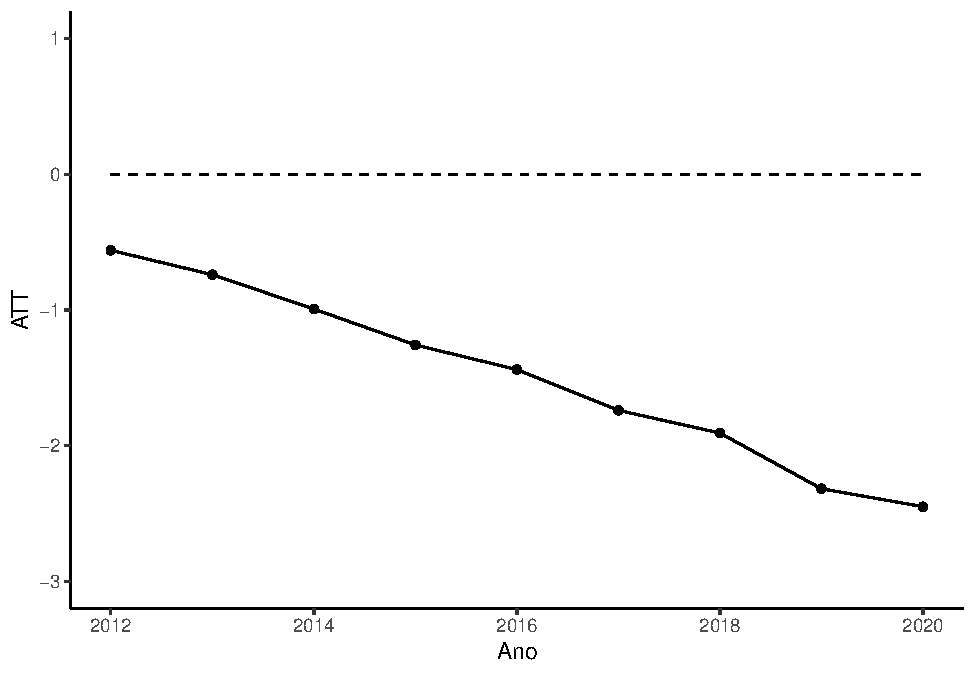
\includegraphics[width=0.8\textwidth]{Figuras/unnamed-chunk-4-1.pdf}

Ao plotar o gráfico, torna-se evidente como a intervenção tem um efeito negativo e crescente, em valor absoluto, ao longo do tempo, resultando em um efeito de -2.45\% no 8º ano pós intervenção. Se desejarmos calcular a média no período, podemos fazê-lo somando os efeitos médios estimados para cada ano: 

$$\gamma = \frac{1}{T}\sum_{t=1}^{T} \Hat{ATT}(t) $$

    \begin{Shaded}
    \begin{Highlighting}[]
    \FunctionTok{mean}\NormalTok{(ATT)}
    \end{Highlighting}
    \end{Shaded}

\begin{verbatim}
## [1] -1.489463
\end{verbatim}

E, portanto, o efeito médio ao longo dos 8 anos é de 1.489\%.

\end{boxA}

\subsubsection{Regressão DID com múltiplos períodos pós-tratamento}

O que acontece se rodarmos a regressão padrão do DiD representada pela equação \eqref{eq:1_regdid} no caso de múltiplos períodos de tratamento? Suponha, portanto, que estamos estimando a regressão abaixo:

\begin{equation}\label{eq:regdid}
    y_{it} = \alpha + \theta d_i + \lambda T_t + \gamma (d_i*T_t) +  \varepsilon_{it}
\end{equation}

onde $T_t = \begin{cases} 1 & t>0 \\ 0 & t=0 \end{cases}$, $d_i = \begin{cases} 1 & i \in \mathcal{D} \\ 0 & c.c. \end{cases}$ e $\mathcal{D}$ representa o conjunto de todos os indivíduos tratados.

Como derivado para o DID 2x2, podemos escrever $\gamma$ como:

\begin{equation*}
\begin{aligned}
\gamma= & E\left[y_{it} \mid d=1, t > 0\right] - E\left[y_{it} \mid d=1, t=0\right] \\
 & - ( E\left[y_{i t} \mid d=\infty, t > 0 \right] - E\left[y_{i t} \mid d=\infty, t=0\right] )
\end{aligned}
\end{equation*}

E pela Lei das Expectativas Iteradas:

\[
\begin{split}
    E\left[y_{i t} \mid d=1, t > 0\right] &= E_t[y_{it} \mid d=1, t=t] \\
    &= \sum_{\tau=1}^{T} P(t=\tau) E[y_{i\tau} \mid d=1] \\
    &=  \sum_{\tau=1}^{T} P(t=\tau) E[y_{i\tau}(1) \mid d=1]
\end{split}
\]

\noindent com P(t=0)=0 pois estamos tirando a esperança condicional de $t>0$.\footnote{$E[y_{it}, d=1, t=t] = E[y_{it}, d=1]$ é um abuso de notação, no fundo estamos definindo que $E[y_{it}] = E[y_i|t=t]$.} 

Vamos assumir incialmente que temos um painel balanceado. Portanto, $P(t=\tau) = 1/T$. Dessa forma, podemos escrever:

\[
\begin{split}
    E\left[y_{i t} \mid d=1, t > 0\right] &= \frac{1}{T} \sum_{\tau=1}^{T} E[y_{i\tau} \mid d=1] \\
    E\left[y_{it} \mid d=1, t = 0\right] &=  E[y_{i0} \mid d=1] \\
      E\left[y_{it} \mid d=0, t > 0\right] &= \frac{1}{T}\sum_{\tau=1}^{T} E[y_{i\tau} \mid d=0] \\
     E\left[y_{i t} \mid d=\infty, t = 0\right] &= E[y_{i0} \mid d=\infty] \\
\end{split}
\]

 \noindent e $\gamma$ será uma função dos $ATT(t)$:

\[\begin{split}
    \gamma &= E\left[y_{i t} \mid d=1, t > 0\right] - E\left[y_{it} \mid d=1, t = 0\right] - ( E\left[y_{it} \mid d=\infty, t > 0\right] - E\left[y_{it} \mid d=\infty, t = 0\right]) \\
    &= \frac{1}{T} \sum_{t=1}^{T} E[y_{it} \mid d=1] - E[y_{i0} \mid d=1] - \left( \frac{1}{T}\sum_{t=1}^{T} E[y_{it} \mid d= \infty] - E[y_{i0} \mid d=\infty]\right)
    \\
    &= \frac{\sum_{t=1}^{T} \{E[y_{it} \mid d=1] - E[y_{i0} \mid d=1]\}}{T} -  \left( \frac{\sum_{t=1}^{T} \{ E[y_{it} \mid d= \infty] - E[y_{i0} \mid d=\infty]\}}{T}\right) \\
    &= \frac{1}{T} \sum_{t=1}^{T}  E[y_{it} - y_{i0}|d=1] - E[y_{it} - y_{i0}|d=\infty] = \frac{1}{T} \sum_{t=1}^{T} \gamma_{t}^{DID} 
\end{split}\]

Se estivermos lidando com um painel balanceado, o parâmetro $\gamma$ da equação \eqref{eq:regdid} representará a média simples dos efeitos médios do tratamento em cada período de tempo. Agora, o que acontecerá se não tivermos em um painel balanceado? Nesse caso, a probabilidade do indivíduo i aparecer no tempo t não será constante (e igual a $1/T$); portanto, estimaremos uma média ponderada dos ATT(t) onde os pesos dependerão da quantidade de indivíduos naquele ano ($N_{gt}$) em relação ao total de indivíduos-ano ($NT = \sum _{g \in G} \sum_{t=1}^{T} N_{gt}$). Você pode demonstrar isso como exercício.

\begin{boxA}

\textbf{Estimando o efeito tratamento com o modelo de DID via MQO}
\vspace{5}

    Voltamos ao exemplo do programa de sustentabilidade cujos dados estão disponíveis na base de dados "base\_MULT\_did.csv". A variável $d$ representa se o município é tratado ou controle e $y$ representa a variação, em porcentagem, da quantidade de energia elétrica usada durante o ano no município.  
    
    Assumiremos que a hipótese de tendências paralelas incondicional é válida (sem a necessidade de nenhum controle). Agora, vamos estimar $\gamma$ da equação \eqref{eq:regdid}. Para isso, vamos criar nossa variável \textit{dummy}:
    
    $T_t = \begin{cases} 1 & ano \geq 2012 \\ 0 & c.c  \end{cases}$.

    \begin{Shaded}
\begin{Highlighting}[]
\NormalTok{df }\OtherTok{\textless{}{-}}\NormalTok{ df }\SpecialCharTok{\%\textgreater{}\%} \FunctionTok{mutate}\NormalTok{(}\AttributeTok{Tt =} \FunctionTok{ifelse}\NormalTok{(ano}\SpecialCharTok{\textgreater{}=}\DecValTok{2012}\NormalTok{, }\DecValTok{1}\NormalTok{, }\DecValTok{0}\NormalTok{))}
\end{Highlighting}
\end{Shaded}

Agora, vamos estimar via MQO a equação abaixo:

\begin{equation*}
    y_{it} = \alpha + \theta d_i + \lambda T_t + \gamma (d_i*T_t) +  \varepsilon_{it}
\end{equation*}

\begin{Shaded}
\begin{Highlighting}[]
\NormalTok{Reg\_did  }\OtherTok{\textless{}{-}} \FunctionTok{lm}\NormalTok{(y }\SpecialCharTok{\textasciitilde{}}\NormalTok{ d}\SpecialCharTok{*}\NormalTok{Tt, }\AttributeTok{data =}\NormalTok{ df)}
\end{Highlighting}
\end{Shaded}

E, finalmente, calcular os desvios padrão robustos à heteroscedasticidade:


    \begin{Shaded}
    \begin{Highlighting}[]
    \CommentTok{\# Load libraries}
    \FunctionTok{library}\NormalTok{(}\StringTok{"lmtest"}\NormalTok{)}
    \FunctionTok{library}\NormalTok{(}\StringTok{"sandwich"}\NormalTok{)}
    
    \CommentTok{\# Robust t test}
    \NormalTok{cov1 }\OtherTok{\textless{}{-}}\NormalTok{ sandwich}\SpecialCharTok{::}\FunctionTok{vcovHC}\NormalTok{(Reg\_did, }\AttributeTok{type =} \StringTok{"HC0"}\NormalTok{)}
    \NormalTok{sd }\OtherTok{=} \FunctionTok{sqrt}\NormalTok{(}\FunctionTok{diag}\NormalTok{(cov1))}
    \FunctionTok{stargazer}\NormalTok{(Reg\_did, }\AttributeTok{type =} \StringTok{"latex"}\NormalTok{, }\AttributeTok{se =} \FunctionTok{list}\NormalTok{(sd),}
              \AttributeTok{title =} \StringTok{"MQO com Erros Padrão Robustos"}\NormalTok{)}
    \end{Highlighting}
    \end{Shaded}

\begingroup
    \fontsize{8pt}{12pt}\selectfont
    \begin{center}
    \begin{tabular}{@{\extracolsep{5pt}}lc} 
    \\[-1.8ex]\hline 
    \hline \\[-1.8ex] 
     & \multicolumn{1}{c}{\textit{Dependent variable:}} \\ 
    \cline{2-2} 
    \\[-1.8ex] & y \\ 
    \hline \\[-1.8ex] 
     d & 6.249$^{***}$ \\ 
      & (0.075) \\ 
      & \\ 
     Tt & $-$6.206$^{***}$ \\ 
      & (0.080) \\ 
      & \\ 
     d:Tt & $-$1.489$^{***}$ \\ 
      & (0.106) \\ 
      & \\ 
     Constant & 9.937$^{***}$ \\ 
      & (0.059) \\ 
      & \\ 
    \hline \\[-1.8ex] 
    Observations & 12,000 \\ 
    R$^{2}$ & 0.424 \\ 
    Adjusted R$^{2}$ & 0.424 \\ 
    Residual Std. Error & 3.750 (df = 11996) \\ 
    F Statistic & 2,949.144$^{***}$ (df = 3; 11996) \\ 
    \hline 
    \hline \\[-1.8ex] 
    \textit{Note:}  & \multicolumn{1}{r}{$^{*}$p$<$0.1; $^{**}$p$<$0.05; $^{***}$p$<$0.01} \\ 
    \end{tabular} 
    \end{center}
\endgroup


   Ou seja:

\[\begin{split}
    \alpha = 9.937 & \hspace{10mm} \theta = 6.249 \\
    \lambda = -6.206 &  \hspace{10mm} \gamma = -1.489
\end{split}\]

A intervenção teve um efeito médio ao longo dos anos de 2012 a 2020 de -1.489\%, i.e., $\gamma = \frac{1}{T} \sum_{t=2012}^{2020} ATT(t)= -1.489$. Ou seja, o programa reduziu o consumo de energia elétrica em aproximadamente 1.49\%, em média, nas cidades expostas a intervenção.

Vale ressaltar que podemos obter o mesmo resultado da seção anterior quando tiramos a média simples de todos os $ATT(t)$, exatamente porque estamos diante de um painel balanceado e porque estamos assumindo que não é necessário controlarmos por nenhuma variável. Entretanto, como argumenta \cite{angrist2009mostly}, poderíamos facilmente estimar a regressão com controles se necessário, além de calcular os erros padrões robustos a heteroscedasticidade e \textit{clusters} para realizar testes de hipóteses corretamente.
    
\end{boxA}

Em um DID com múltiplos períodos pós-tratamento e \textbf{todos os indivíduos do grupo de tratamento sendo tratado ao mesmo tempo}, a regressão nos retornará o efeito médio do tratamento ao longo dos anos pós-tratamento. Se tivermos em um painel balanceado, essa será uma média simples, ou então uma média ponderada com o peso sendo o tamanho relativo do grupo no caso de painéis desbalanceados. Em ambos os casos, diferente do DID escalonado estudado nas seções futuras, não temos o problema de estimar consistentemente uma média dos $ATT(t)$ informativa.   

No entanto, mesmo estimando consistentemente essa média dos efeitos ao longo do tempo, surge a questão: isso é realmente o que desejamos estimar? Embora a abordagem mais óbvia seja calcular a média simples dos efeitos em cada período de tempo, essa medida pode ''esconder'' informações relevantes para a análise da intervenção, já que ela não nos releva informações sobre a dinâmica do efeito do tratamento ao longo do tempo. 

\begin{figure}[!h]
\centering
\begin{tikzpicture}

\coordinate (0) at (-1,0);
\coordinate (F) at (11,0);

\draw[->] (0) -- (F);
\foreach \x in {0,2,4,6, 8, 10}
    \draw(\x cm,3pt) -- (\x cm,-3pt);

\foreach \i \j in {0/0,2/1,4/2,6/3, 8/4, 10/5}
    \draw (\i,0) node[below=3pt] {\j} ;

\draw[dashed] (1,-1) -- (1,5);
\draw (1, -1.5) node[black] {Intervenção};


\foreach \x in {2, 4, ...,10} {
            \filldraw [color=blue] (\x,0.3*\x) circle (2pt);
            \filldraw [color=red] (\x,1.75) -- ++(4pt,0) -- ++(-2pt,-4pt) -- cycle;
        }

\foreach \x in {2, 4} {  
    \filldraw [color=black] (\x,1*\x) rectangle ++(4pt,4pt);
}

\filldraw [color=black] (6,1.5) rectangle ++(4pt,4pt);

\foreach \x in {8, 10} {  
    \filldraw [color=black] (\x-0.05,-0.05) rectangle ++(4pt,4pt);
}



\node[draw,align=left,fill=white] at (1,4) {%
    \textbf{Legenda}\\
    \textcolor{blue}{$\bullet$} --- $ATT(t)$ crescente\\
    \textcolor{red}{$\blacktriangle$} --- $ATT(t)$ constante\\
    \textcolor{black}{$\blacksquare$} --- $ATT(t)>0$ curto prazo
};

\end{tikzpicture}
\caption{ATT(t)} \label{fig:ATT(t)}
\end{figure}

A Figura \ref{fig:ATT(t)} representa três exemplos de dinâmicas para o $ATT(t)$ com a mesma média. A primeira, em azul, mostra um efeito crescente ao longo do tempo de exposição ao tratamento, enquanto a segunda (em vermelho) exibe um efeito constante. A última (em preto) ilustra um efeito significativo no curto prazo, mas nenhum efeito no longo prazo. Ao estimarmos $\gamma$ para cada uma dessas intervenções por MQO, obteríamos a mesma estimativa para cada caso. Para contornarmos o problema, podemos estimar de forma simples os $ATT(t)$ interagindo nossa \textit{dummy} de tratamento com uma \textit{dummy} pra cada ano.

\subsubsection{Regressão com Dummies de tempo}

Para conseguirmos estimar cada um dos $ATT(t)$, que serão iguais a cada um dos  $\gamma_t$ na equação \eqref{eq:did_mult_dumies}, definiremos um conjunto de dummies de tempo:

\[
\begin{split}
    \mathbbm{1}_{\tau} = \begin{cases} 1 & t = \tau \\ 0 & c.c. \end{cases}
\end{split}
\]

\noindent Considere o exemplo de uma intervenção feita no ano 2012. Nesse caso, $t=0$ seria o ano de 2011 e, em 2011, $\mathbbm{1}_{0} = 1$ e $\mathbbm{1}_{1} = \mathbbm{1}_{2} = ... \mathbbm{1}_{T} = 0$. Temos, então:

\begin{equation}\label{eq:did_mult_dumies}
    y_{igt} = \alpha_g + \theta_t + \sum_{t=t_0+1}^{T} \gamma_t  \mathbbm{1}_{\tau} d * T_t + \varepsilon_{igt} 
\end{equation}

\noindent onde $g \in \{\infty,1\}$ determina se o indivíduo é do grupo de controle (i.e., $g= \infty$) ou do grupo de tratamento (i.e., $g=1$). Dessa forma, como mostrado por \cite{angrist2009mostly}, se as hipóteses 1-4 da seção anterior forem satisfeitas:

$$ \gamma_t = ATT(t)$$

\noindent e, do mesmo modo que na regressão sem dummies, conseguimos facilmente calcular os erros padrões robustos a heterocedasticidade e clusters.

Isso pode ser demonstrado pelo mesmo procedimento da seção anterior. Teremos que:

\[
\begin{split}
   \gamma_t =& E[y_{it} - y_{i0}|d=1] - E[y_{it} - y_{i0}|d=\infty] \\
                    =&\underbrace{E[y_{it}(1) - y_{it}(\infty)|d=1]}_{ATT(t)} \\
                    &- ( E[y_{it}(\infty) - y_{i0}(\infty)|d=1] - E[y_{it}(\infty) - y_{i0}(\infty)|d=\infty])
\end{split}
\]

\noindent onde, sob tendências paralelas, $E[y_{it}(\infty) - y_{it}(\infty)|d=1] - E[y_{it}(\infty) - y_{i0}(\infty)|d=\infty] = 0$.

Além disso, como estimamos consistentemente cada ATT(t), podemos calcular qualquer média ponderada dos ATT(t) que seja interessante para a análise da intervenção, isto é:

$$ \Gamma = \sum_{t>0} w(t) ATT(t) $$

\noindent onde $w(t)$ é um peso arbitrariamente escolhido tal que $\sum_{t>0} w(t) = 1$ e $w(t) \geq 0$.

Entretanto, qual média ponderada seria interessante? Como argumentado por \cite{callaway2021difference}, isso depende muito das características específicas da intervenção avaliada e dos objetivos da pesquisa. Por exemplo:

\begin{itemize}
    \item Se quisermos avaliar o efeito médio ao longo de todos os anos da análise, poderíamos determinar um peso igual para cada ano da amostra, isto é, $w(t) = 1/T$ (exatamente como na regressão sem dummies).

    \item Se quisermos ver o efeito acumulado durante todos os anos da intervenção, definiríamos: $w(t) = 1$ para todo $t$.
    \item Agora, se estivermos interessados em avaliar o efeito do tratamento no curto prazo, poderíamos definir que o curto prazo seria até 4 anos após a intervenção e $w(t) = \begin{cases}
    1/4 & t \leq 4 \\ 0 & t > 4 
    \end{cases}$.
    \item Ou, ainda, se quisermos avaliar se o efeito de curto prazo ($\leq 4$ anos) é maior que o efeito de longo prazo ($> 4$ anos), definiríamos $w(t) = \begin{cases}
    -\frac{1}{4} & t \leq 4 \\ \frac{1}{T-4}  & t > 4 
    \end{cases}$
\end{itemize}

A inferência sobre o parâmetro $\Gamma$ também não é difícil, uma vez que os erros padrão do estimador podem ser calculados rapidamente com o \textit{Delta method}. %\cite{sun2021estimating}, estudado na seção \ref{sec:Sun}, seguirá o mesmo raciocínio para corrigir o problema quando temos uma DID escalonado.

\begin{boxA}

    \textbf{Estimando $ATT(t)$ com DID via MQO}

    \vspace{5mm}

    Primeiro, vamos transformar a variável \textit{ano} em \textit{factors}, para assim, gerar \textit{dummies} pra cada ano com a função \textit{lm}.
    
    \begin{Shaded}
    \begin{Highlighting}[]
    \NormalTok{df }\OtherTok{\textless{}{-}}\NormalTok{ df }\SpecialCharTok{\%\textgreater{}\%} \FunctionTok{mutate}\NormalTok{(}\AttributeTok{Tt =} \FunctionTok{ifelse}\NormalTok{(ano }\SpecialCharTok{\textgreater{}=} \DecValTok{2012}\NormalTok{, }\DecValTok{1}\NormalTok{, }\DecValTok{0}\NormalTok{),}
                        \AttributeTok{ano =} \FunctionTok{as.factor}\NormalTok{(ano) }\CommentTok{\#criar Dummies}
    \NormalTok{                    )}
    \end{Highlighting}
    \end{Shaded}

    Agora vamos estimar a regressão \eqref{eq:did_mult_dumies}, isto é:

    $$     y_{ist} = \alpha_s + \theta_t + \sum_{t=t_0+1}^{T} \gamma_t  \mathbbm{1}_{\tau} d * T_t + \varepsilon_{ist}  $$

    \begin{Shaded}
    \begin{Highlighting}[]
    \NormalTok{Reg\_did }\OtherTok{\textless{}{-}} \FunctionTok{lm}\NormalTok{(y }\textasciitilde{} \FunctionTok{as.factor}\NormalTok{(d) }\SpecialCharTok{+}\NormalTok{ ano }\SpecialCharTok{+}\NormalTok{ ano}\SpecialCharTok{:}\NormalTok{d}\SpecialCharTok{:}\NormalTok{Tt, }
    \AttributeTok{data =}\NormalTok{ df)}
    \end{Highlighting}
    \end{Shaded}

    E, como sempre, calcular os erros padrão robustos e gerar a tabela.
    
    \begin{Shaded}
    \begin{Highlighting}[]
    \FunctionTok{library}\NormalTok{(}\StringTok{"lmtest"}\NormalTok{)}
    \FunctionTok{library}\NormalTok{(}\StringTok{"sandwich"}\NormalTok{)}

    \CommentTok{\# Robust t test}
    \NormalTok{cov1 }\OtherTok{\textless{}{-}}\NormalTok{ sandwich}\SpecialCharTok{::}\FunctionTok{vcovHC}\NormalTok{(Reg\_did, }\AttributeTok{type =} \StringTok{"HC0"}\NormalTok{)}
    \NormalTok{sd\_robust }\OtherTok{=} \FunctionTok{sqrt}\NormalTok{(}\FunctionTok{diag}\NormalTok{(cov1))}
    \CommentTok{\# Especifique as variáveis que você deseja incluir na tabela}

    \CommentTok{\# Extraia os coeficientes relevantes}
    \NormalTok{coef\_names }\OtherTok{\textless{}{-}} \FunctionTok{names}\NormalTok{(}\FunctionTok{coef}\NormalTok{(Reg\_did))}
    \NormalTok{vars\_to\_include }\OtherTok{\textless{}{-}} \FunctionTok{grep}\NormalTok{(}\FunctionTok{paste0}\NormalTok{(}\StringTok{"ano}\SpecialCharTok{\textbackslash{}\textbackslash{}}\StringTok{d\{4\}:d:Tt"}\NormalTok{)},
                            \NormalTok{coef\_names, }\AttributeTok{value =} \ConstantTok{TRUE}\NormalTok{)}
    

    \CommentTok{\# Gere a tabela usando stargazer}
    \FunctionTok{stargazer}\NormalTok{(Reg\_did, }\AttributeTok{type =} \StringTok{"latex"}\NormalTok{, }\AttributeTok{se =} \FunctionTok{list}\NormalTok{(sd\_robust), }
              \AttributeTok{title =} \StringTok{"MQO com Erros Padrão Robustos"}\NormalTok{)}
    \end{Highlighting}
    \end{Shaded}

    Como usamos a fórmula "ano:d:Tt", $\gamma_{2012} = $ será mostrado como "ano2012:d:Tt", $\gamma_{2013} = $ será como "ano2012:d:Tt", e assim por diante. Além disso, vamos ocultar as estimativas dos efeitos fixos de tempo e de indivíduo, dado o alto número de regressores.

    \begingroup
        \fontsize{8pt}{12pt}\selectfont
        \begin{center}
         \begin{tabular}{@{\extracolsep{5pt}}cc} 
         \\[-1.8ex]\hline 
         \hline \\[-1.8ex] 
          & \multicolumn{1}{c}{\textit{Dependent variable:}} \\ 
         \cline{2-2} 
         \\[-1.8ex] & y \\ 
         \hline \\[-1.8ex] 
            $\vdots$ & $\vdots$ \\
            & \\
          ano2012:d:Tt & $-$0.561$^{***}$ \\ 
           & (0.103) \\ 
          ano2013:d:Tt & $-$0.740$^{***}$ \\ 
           & (0.105) \\ 
          ano2014:d:Tt & $-$0.993$^{***}$ \\ 
           & (0.108) \\ 
          ano2015:d:Tt & $-$1.258$^{***}$ \\ 
           & (0.112) \\ 
          ano2016:d:Tt & $-$1.439$^{***}$ \\ 
           & (0.116) \\ 
          ano2017:d:Tt & $-$1.740$^{***}$ \\ 
           & (0.120) \\ 
          ano2018:d:Tt & $-$1.907$^{***}$ \\ 
           & (0.123) \\ 
          ano2019:d:Tt & $-$2.318$^{***}$ \\ 
           & (0.132) \\ 
          ano2020:d:Tt & $-$2.450 \\ 
           & (0.132) \\ 
          Constant & 9.937$^{***}$ \\ 
           & (0.059) \\ 
         \hline \\[-1.8ex] 
         Observations & 12,000 \\ 
         R$^{2}$ & 0.907 \\ 
         Adjusted R$^{2}$ & 0.907 \\ 
         Residual Std. Error & 1.509 (df = 11980) \\ 
         F Statistic & 6,141.730$^{***}$ (df = 19; 11980) \\ 
         \hline 
         \hline \\[-1.8ex] 
         \textit{Note:}  & \multicolumn{1}{r}{$^{*}$p$<$0.1; $^{**}$p$<$0.05; $^{***}$p$<$0.01} \\ 
         \end{tabular} 
        \end{center}
     \endgroup

Ou seja, temos que:

\[\begin{split}
    \gamma_{2012} &= -0.561,  \gamma_{2013} = -0.740, \gamma_{2014} = 0.993, \gamma_{2015} = -1,258 \\
    \gamma_{2016} &= -1.439,  \gamma_{2017} = -1.740, \gamma_{2018} = 1.907, \gamma_{2019} = -2.318 \\
    \gamma_{2020} &= -2.45
\end{split}\]

Agora, podemos estimar qualquer combinação dos $ATT(t)$ ($\gamma_t$).

$$\Gamma = \sum_{t=t_0+1}^{T} w_t \gamma_t$$

Primeiro, vamos armazenar todos os coeficientes que representam os ATT(t) em um vetor.

\begin{Shaded}
\begin{Highlighting}[]
\NormalTok{ATT }\OtherTok{=}\NormalTok{ Reg\_did}\SpecialCharTok{$}\NormalTok{coefficients[}\FunctionTok{paste0}\NormalTok{(}\StringTok{"ano"}\NormalTok{, }\DecValTok{2012}\SpecialCharTok{:}\DecValTok{2020}\NormalTok{, }\StringTok{":d:Tt"}\NormalTok{)]}
\end{Highlighting}
\end{Shaded}

E vamos calcular $\Gamma$ e seus desvios padrões usando o método delta. \footnote{Para mais informações sobre o método delta e como usar veja: \cite{ver2012invented}.} Para começar, podemos calcular a média simples, ou seja $w(t) = \frac{1}{T} = \frac{1}{9}$. Logo:

$$ \Gamma = \frac{1}{9} \sum_{t=2012}^{2020} \gamma_t $$

\begin{Shaded}
\begin{Highlighting}[]
\NormalTok{wt}\OtherTok{=} \DecValTok{1}\SpecialCharTok{/}\DecValTok{9} \CommentTok{\#(1/T)}

\NormalTok{Gamma}\OtherTok{=} \FunctionTok{sum}\NormalTok{(wt}\SpecialCharTok{*}\NormalTok{ATT)}

\CommentTok{\#calculado Sd via Delta method}
\NormalTok{Grad }\OtherTok{=} \FunctionTok{matrix}\NormalTok{(}\FunctionTok{c}\NormalTok{(}\FunctionTok{rep}\NormalTok{(}\DecValTok{0}\NormalTok{, }\DecValTok{12}\NormalTok{), }\FunctionTok{rep}\NormalTok{(wt,}\DecValTok{8}\NormalTok{)), }\AttributeTok{ncol =} \DecValTok{1}\NormalTok{)}
\NormalTok{Sd\_Gamma }\OtherTok{=} \FunctionTok{sqrt}\NormalTok{(}\FunctionTok{t}\NormalTok{(Grad)}\SpecialCharTok{\%*\%}\NormalTok{cov1}\SpecialCharTok{\%*\%}\NormalTok{Grad)}
\CommentTok{\# Calcula o p\_valor}
\NormalTok{  valor\_t }\OtherTok{\textless{}{-}}\NormalTok{ (Gamma)}\SpecialCharTok{*}\FunctionTok{sqrt}\NormalTok{(}\DecValTok{12000}\NormalTok{) }\SpecialCharTok{/}\NormalTok{Sd\_Gamma}
\NormalTok{  gl }\OtherTok{\textless{}{-}}\NormalTok{ Reg\_did}\SpecialCharTok{$}\NormalTok{df.residual}
\NormalTok{  valor\_p }\OtherTok{\textless{}{-}} \DecValTok{2} \SpecialCharTok{*} \FunctionTok{pt}\NormalTok{(}\FunctionTok{abs}\NormalTok{(valor\_t), }\AttributeTok{df=}\NormalTok{gl, }\AttributeTok{lower.tail=}\ConstantTok{FALSE}\NormalTok{)}
\end{Highlighting}
\end{Shaded}

\begin{Shaded}
\begin{Highlighting}[]
\FunctionTok{print}\NormalTok{(}\FunctionTok{c}\NormalTok{(Gamma, Sd\_Gamma, valor\_p))}
\end{Highlighting}
\end{Shaded}

\begin{verbatim}
## [1]   "Gamma"       "Sd"     "P_valor"
## [1] -1.48946344  0.0804382  0.00000000
\end{verbatim}

Como esperado, estimamos o mesmo valor que o obtido com a regressão DID padrão. O desvio padrão também foi muito semelhante, e rejeitamos a hipótese de efeito zero.

Entretanto, como discutido, pode ser interessante analisar outros fatores. Por exemplo, será que o efeito de médio a longo prazo é maior do que o efeito de curto prazo (até o quarto período após o tratamento)? Para investigar isso, vamos definir:

$$ w_t = \begin{cases} -1/4 & t \leq 4 \\ \text{  } 1/4 & t > 4 \end{cases} $$

E, como os ATT(t) são negativos, se $\Gamma > 0$, o efeito de longo prazo seria menor, em valor absoluto, do que o efeito de curto prazo. Se $\Gamma < 0$, os efeitos de longo prazo seriam maiores. Por fim, se $\Gamma = 0$, o efeito, em média, é igual no longo e no curto prazo.


\begin{Shaded}
\begin{Highlighting}[]
\NormalTok{wt }\OtherTok{=} \FunctionTok{c}\NormalTok{(}\FunctionTok{rep}\NormalTok{(}\SpecialCharTok{{-}}\DecValTok{1}\SpecialCharTok{/}\DecValTok{4}\NormalTok{, }\DecValTok{4}\NormalTok{), }\FunctionTok{rep}\NormalTok{(}\DecValTok{1}\SpecialCharTok{/}\DecValTok{4}\NormalTok{,}\DecValTok{5}\NormalTok{))}

\NormalTok{Gamma }\OtherTok{=} \FunctionTok{sum}\NormalTok{(wt}\SpecialCharTok{*}\NormalTok{ATT)}
\CommentTok{\#calculado Sd via Delta method}
\NormalTok{Grad }\OtherTok{=} \FunctionTok{matrix}\NormalTok{(}\FunctionTok{c}\NormalTok{(}\FunctionTok{rep}\NormalTok{(}\DecValTok{0}\NormalTok{, }\DecValTok{12}\NormalTok{), wt), }\AttributeTok{ncol =} \DecValTok{1}\NormalTok{)}
\NormalTok{Sd\_Gamma }\OtherTok{=} \FunctionTok{sqrt}\NormalTok{(}\FunctionTok{t}\NormalTok{(Grad)}\SpecialCharTok{\%*\%}\NormalTok{cov1}\SpecialCharTok{\%*\%}\NormalTok{Grad)}
\CommentTok{\# Calcula o p\_valor}
\NormalTok{  valor\_t }\OtherTok{\textless{}{-}}\NormalTok{ (Gamma)}\SpecialCharTok{*}\FunctionTok{sqrt}\NormalTok{(}\DecValTok{12000}\NormalTok{) }\SpecialCharTok{/}\NormalTok{Sd\_Gamma}
\NormalTok{  gl }\OtherTok{\textless{}{-}}\NormalTok{ Reg\_did}\SpecialCharTok{$}\NormalTok{df.residual}
\NormalTok{  valor\_p }\OtherTok{\textless{}{-}} \DecValTok{2} \SpecialCharTok{*} \FunctionTok{pt}\NormalTok{(}\FunctionTok{abs}\NormalTok{(valor\_t), }\AttributeTok{df=}\NormalTok{gl, }\AttributeTok{lower.tail=}\ConstantTok{FALSE}\NormalTok{)}
\end{Highlighting}
\end{Shaded}

\begin{Shaded}
\begin{Highlighting}[]
\FunctionTok{print}\NormalTok{(}\FunctionTok{c}\NormalTok{(Gamma, Sd\_Gamma, valor\_p))}
\end{Highlighting}
\end{Shaded}


\begin{verbatim}
## [1]    "Gamma"      "Sd"     "P_valor"
## [1] -1.57538221  0.07025662  0.00000000
\end{verbatim}

E, portanto, como $\Gamma < 0$, o efeito de longo prazo tem maior intensidade do que o efeito de curto prazo. Também poderíamos ter chegado a essa conclusão apenas plotando o gráfico dos ATT(t), como na seção anterior. No entanto, com esse procedimento, além de obtermos facilmente os erros padrão para testes de hipóteses, podemos usar o mesmo raciocínio para avaliar outras formas interessantes. Por exemplo, podemos definir $w(t) = 1$ para todo $t$ e calcular o efeito acumulado ao longo dos anos.
    
\end{boxA}

\subsection{Regressão DID com múltiplos períodos pré-tratamento}

Nesta seção, será estudado o modelo de diferenças-em-diferenças com mais de um período pré-tratamento. Os períodos pré-tratamento serão definidos com índices menores ou iguais a zero, ou seja, $0, -1, -2, ...$, e o único período pós-tratamento será definido com índice $1$. A figura abaixo representa graficamente os períodos antes e depois da intervenção.

\begin{figure}[!htp]
    \centering
    \begin{tikzpicture}[very thick, black, scale=0.6]
    \centering
    
    \coordinate (0) at (-1,0);
    \coordinate (F) at (11.5,0);
    
    \draw[->] (0) -- (F);
    \foreach \x in {0,2,4,6, 8, 10}
        \draw(\x cm,3pt) -- (\x cm,-3pt);
    
    \foreach \i \j in {0/-4,2/-3,4/-2,6/-1, 8/0, 10/1}
        \draw (\i,0) node[below=3pt] {\j} ;
    
    \draw[dashed] (9,-1) -- (9,3);
    \draw (9, -1.5) node[black] {Intervenção};
    
    \fill[color=Dandelion!20] rectangle (9,0) -- (9,3) -- (11,3) -- (11,0); % Studies
    \draw (4,1.5) node[black] {Pré-intervenção} 
    \end{tikzpicture}
\end{figure}

Diferentemente do modelo com múltiplos períodos pós-intervenção, a definição do efeito do tratamento (ATT) não dependerá do tempo, pois há apenas um período pós-intervenção. Portanto, o ATT se mantém igual a:

$$ ATT = E[y_i(1) - y_i(\infty) | d=1] $$

A principal diferença se dará na hipótese de tendências paralelas, que agora deverá ser válida para todos os períodos pré-tratamento. Semelhante ao que foi feito na seção \ref{sec:DID_DIF_MEDIA}, derivaremos a condição suficiente da tendência paralela no caso com mais de um período pré-tratamento. Como temos mais de um período pré-tratamento, a diferença será feita entre o período pós-tratamento e a média de todos os períodos pré-tratamento. Defina, então, $N_{t\leq 0}$ como a quantidade total de períodos pré-intervenção. Teremos, sob a hipótese de não antecipação (i.e. $\forall t \leq 0$, $y_{it} = y_{it}(\infty)$:

\[
\begin{split}
    \Delta_{Tr} &= E[y_{i1}(1)|d_i=1] - E\left[\frac{\sum_{t\leq 0} y_{it}(\infty)}{N_{t\leq 0}}|d_i=1\right] \\
    \Delta_{Cr} &= E[y_{i1}(\infty)|d_i=\infty] - E\left[\frac{\sum_{t\leq 0} y_{it}(\infty)}{N_{t\leq 0}}|d_i=\infty\right]. \\
\end{split}
\]

\noindent A segunda diferença continua a mesma, ou seja:

\[\begin{split}
    \gamma^{DID} & = \Delta_{Tr} - \Delta_{Cr} \\
    & = \left(E[y_{i1}(1) | d_i = 1] - E\left[\frac{\sum_{t\leq0} y_{it}(\infty)}{N_{t\leq0}} | d_i = 1\right]\right) \\
    & \hspace{10mm}- \left(E[y_{i1}(\infty) | d_i = 0] - E\left[\frac{\sum_{t\leq0} y_{it}(\infty)}{N_{t\leq0}} | d_i = 0\right]\right)\\
\end{split}
\]

Somando e subtraindo  $\textcolor{red}{E[y_{i1}(\infty) | d_i = 1]}$:

\begin{equation*}
    \begin{split}
     \gamma^{DID} & = \underbrace{E[y_{i1}(1) - y_{i1}(\infty) | d_i = 1]}_{ATT} \\
     & \hspace{3mm} + E\left[y_{i1}(\infty) - \frac{\sum_{t\leq0} y_{it}(\infty)}{N_{t\leq0}} | d_i = 1\right] - E\left[y_{i1}(\infty) - \frac{\sum_{t\leq0} y_{it}(\infty)}{N_{t\leq0}} | d_i = 0\right].
\end{split}
\end{equation*}

Portanto, para que $\gamma^{DID}$ seja igual ao $ATT$, é necessário que:

\begin{equation}\label{eq:TP_mult_pre_0}
     E\left[y_{i1}(\infty) - \frac{\sum_{t\leq0} y_{it}(\infty)}{N_{t\leq0}} | d_i = 1\right] = E\left[y_{i1}(\infty) - \frac{\sum_{t\leq0} y_{it}(\infty)}{N_{t\leq0}} | d_i = 0\right]
\end{equation}

Usando álgebra, podemos mostrar que essa hipótese é equivalente à hipótese de tendências paralelas convencional em todos os períodos pré-tratamento. Primeiro, vamos mostrar que a diferença $E\left[y_{i1}(\infty) - \frac{\sum_{t\leq0} y_{it}(\infty)}{N_{t\leq0}} | d_i\right]$ é equivalente à média das diferenças para todos os períodos pré-tratamento:

\[
\begin{split}
    E\left[y_{i1}(\infty) - \frac{\sum_{t\leq0} y_{it}(\infty)}{N_{t\leq0}} | d_i\right] &=  E\left[ \textcolor{red}{\frac{N_{t\leq0}}{N_{t\leq0}}} y_{i1}(\infty) - \frac{\sum_{t\leq0} y_{it}(\infty)}{N_{t\leq0}} | d_i\right] \\
    &= E\left[ \frac{\sum_{t\leq 0} y_{i1}(\infty)}{N_{t\leq0}} - \frac{\sum_{t\leq0} y_{it}(\infty)}{N_{t\leq0}} | d_i\right] \\
    &= \frac{\sum_{t\leq0}  E\left[ y_{i1}(\infty) -y_{it}(\infty) | d_i\right]}{N_{t\leq 0}}
\end{split}
\]

Ou seja, usando a igualdade acima e a igualdade dada na equação \eqref{eq:TP_mult_pre_0}:

\[
\begin{split}
    \frac{\sum_{t\leq0}  E\left[ y_{i1}(\infty) -y_{it}(\infty) | d_i=1\right]}{N_{t\leq 0}} - \frac{\sum_{t\leq0}  E\left[ y_{i1}(\infty) -y_{it}(\infty) | d_i=0\right]}{N_{t\leq 0}} &= 0 \\
    \frac{1}{N_{t\leq0}}  \sum_{t \leq 0} \big[ E\left[ y_{i1}(\infty) - y_{it}(\infty) | d_i=1\right] - E\left[y_{i1}(\infty) - y_{it}(\infty) | d_i=0\right] \big] &=0
\end{split}
\]

E, portanto, para que um DID funcione com múltiplos períodos pré-tratamento, a média simples da diferença entre as tendências do grupo de controle e tratamento deve ser igual a zero. Essa hipótese pode soar um pouco estranha, pois não é necessário que a tendência paralela seja válida para cada período, apenas que a média simples delas em relação a todos os períodos seja igual para tratados e controles. 

Pela dificuldade de interpretar essa hipótese, muitos trabalhos assumem uma hipótese suficiente, porém mais restritiva, de que para todos os períodos de pré-tratamento, as tendências dos grupos de tratamento e controle são paralelas:

$$\forall t \leq 0, \text{ } E[y_{i1}(\infty) - y_{it}(\infty) | d_i=1] = E[y_{i1}(\infty) - y_{it}(\infty) | d_i=0]$$

\section{Diferenças-em-Diferenças escalonado}

\subsection{O que é um DID escalonado?}

O DID escalonado assemelha-se ao DID múltiplo discutido anteriormente. Contudo, em vez de todos os indivíduos serem tratados simultaneamente, grupos são tratados em diferentes momentos no tempo. Considere o estudo do efeito de uma política econômica, como um aumento no salário mínimo, em diferentes estados de um país. Ao invés de implementar o aumento do salário mínimo de uma só vez em todos os estados, ele é aplicado em estados diferentes em momentos distintos. Por exemplo, é implementado em 2018 em um grupo de estados, em 2019 em outro grupo, e em 2020 o restante dos estados tem o salário mínimo aumentado. Neste contexto, após 2018, o tratamento é escalonado até que todos (ou parte) dos estados sejam tratados.

Os períodos antes do primeiro grupo ser tratado, nos quais nenhum grupo é tratado, serão chamados de período pré-tratamento. Os demais períodos serão períodos pós-tratamento. Os indivíduos tratados pela primeira vez no períodos $t=g$, constituirão o grupo de tratamento $g$. Já o grupo não tratado em nenhum período chamaremos de \textit{never treated} (ou nunca tratados) e denotaremos por $\infty$. $G$ denotará o conjunto de todos os grupos tratados, ou seja, se $i \in g$ e $g \in G$ significa que o indivíduo $i$ pertence ao grupo que foi tratado pela primeira vez no período $t=g$.

\subsection{Aumentando o modelo de resultados potenciais}

Assim como para o DID com múltiplos períodos, aqui será necessário definir ATT para cada período do tempo. No entanto, o resultado potencial pode depender do momento em que o indivíduo recebe o tratamento. Ser exposto à intervenção antes ou depois pode ter efeitos diferentes. Portanto, definiremos cada resultado potencial do indivíduo especificamente ao caso em que ele tivesse sido tratado pela primeira vez no período g, denotado por $y_{it}(g)$. 

Por exemplo, considere uma intervenção onde cada estado do Brasil tem seu salário mínimo aumentado. A exposição foi escalonada entre os anos de 2012 a 2014. O estado de São Paulo ($i=SP$), por exemplo,  terá quatro resultados potenciais diferentes para cada período $t$: um para o caso em que ele é tratado pela primeira vez em 2012, ou seja, $y_{SP,t}(2012)$; outro para o caso em que ele é tratado em 2013, $y_{SP,t}(2013)$; um para o caso em que é tratado pela primeira vez em 2014, $y_{SP,t}(2014)$; e, por fim, para caso não tenha mudado o salário mínimo em nenhum desses anos, $y_{SP,t}(\infty)$. 

Novamente, apenas observamos um dos resultados potenciais para cada indivíduo, isto é, no nosso exemplo, se SP mudar seu salário mínimo em 2014, apenas $y_{(SP, t)} (2014)$ será observado. 

Então, denotaremos agora não só um ATT para cada período do tempo, mas, para cada $t$, um ATT para cada período de início de tratamento $g$. Denotaremos o ATT como:

    $$ ATT(g,t) = E[y_{it}(g) - y_{it}(\infty) | d = g]. $$

\noindent que representa o efeito médio do tratamento no período $t$ para o grupo tratado pela primeira vez no período $g$.

Todos as soluções da literatura, de alguma forma, passarão pela estimação de cada $ATT(g,t)$ de forma análoga a um DID padrão (2x2). Ou seja, as hipóteses e, principalmente, a interpretação dos resultados se assemelham muito aos casos visitados nas seções anteriores. Todas essas soluções requerem que tenhamos tendências paralelas, com algumas poucas variações entre as hipóteses. Porém, o mais importante é que, em  todas as soluções, precisamos ter tendências paralelas para todos os resultados potenciais em todos os períodos de tempo. Em outras palavras, precisaremos de tendências paralelas para $y_{it}(g)$ para todo $t$ e para todo $g \in G \cup \{\infty\}$.

Nesta seção, definiremos as hipóteses para um DID escalonado sem controles, para que os estimadores da literatura acabam por ser muito semelhantes. Quando estivermos destrinchando cada um dos diferentes estimadores, comentaremos as diferenças de hipóteses entre eles e os casos em que necessitaremos de hipóteses mais restritivas do que as apresentadas nesse momento. Essas terão relação, principalmente, com as tendências paralelas condicionais que cada estimador assume.

\begin{boxB}
\begin{enumerate}
    \item \textbf{SUTVA}: O resultado potencial no caso de não tratamento não é afetado pela alocação do tratamento sobre outros indivíduos.
    \item \textbf{Não antecipação}: $\forall i$ e $g \in \{1,2, ..., G\} \cup \{\infty\}$,  $y_{i0} = y_{i0}(g) =   y_{i0}(\infty)$.
    \item \textbf{Irreversibilidade do Tratamento}: $\forall t \geq g, y_{it} = y_{it}(g)$. 
    \item \textbf{Tendências Paralelas para todos os grupos}: 
    $$ \forall t \text{ e } \forall g, \text{ } E[y_{it}(\infty) - y_{i0}(\infty) | d=g] = E[y_{it}(\infty) - y_{i0}(\infty) | d_i = \infty] $$
\end{enumerate}

\end{boxB}

Podemos estimar os $ATT(g, t)$ para cada período de forma semelhante ao DID múltiplo, mas separadamente para cada um dos grupos. Ou seja, para o grupo tratado pela primeira vez em $t=g$:

\[
\begin{split}
    \gamma_{gt}^{DID} &= (E[y_{it} |d = g] -  E[y_{i0} |d = g]) - (E[y_{it} |d = \infty] -  E[y_{i0} |d = \infty]) \\
    &= E[y_{it}(g) - y_{i0}(\infty) | d=g]  - E[y_{it}(\infty) - y_{i0}(\infty) | d_i = \infty] \\
    &= \underbrace{E[y_{it}(g) - y_{it}(\infty) | d=g]}_{ATT(g,t)} \\
    & \hspace{5\infty} + E[y_{it}(\infty) - y_{i0}(\infty) | d=g] - E[y_{it}(\infty) - y_{i0}(\infty) | d_i = \infty] \\
\end{split}\]

\noindent onde da segunda para terceira linha somamos e subtraímos $E[y_{it}(\infty)|d=g]$. Sob as hipóteses 1-4, temos que $\gamma_{gt}^{DID} = ATT(g,t)$. Observe que, para estimarmos o ATT(g,t) consistentemente sob a hipótese de tendências paralelas não condicionais, o procedimento é exatamente igual ao discutido nas seções anteriores, mas realizamos a estimativa separadamente para cada grupo de exposição.

E, portanto, um estimador consistente seria:

$$ \hat{\gamma}^{DID}_{gt} = (\Bar{y}_{gt} - \Bar{y}_{g0}) - (\Bar{y}_{\infty t} - \Bar{y}_{\infty 0}) $$

Note que, sob as hipóteses 1-4, temos que $\hat{\gamma}^{DID}_{gt}  \xrightarrow{p} ATT(g,t)$. E, dado que temos um estimador consistente para cada $ATT(g,t)$, podemos, como fizemos para o DID múltiplo, estimar qualquer média ponderada deles. Então, qual seria o problema de um DiD escalonado? O problema surge quando tentamos estimá-lo usando um TWFE, como nos casos anteriores. Na próxima seção, vamos detalhar os problemas de se rodar um DID escalonado em um modelo TWFE.

\begin{boxA}
    Vamos continuar com nosso exemplo sobre o programa de sustentabilidade nos municípios brasileiros. Entretanto, agora o programa será implementado de maneira escalonada. Ou seja, parte dos municípios serão expostos à intervenção em 2012; outra parte em 2014; uma terceira parte em 2016, o restante em 2018. Assumiremos que alguns municípios não serão tratados em nenhum momento.

    A base com os dados fictícios se encontra no arquivo "base\_stagger\_did.csv". Vamos primeiro observar o tamanho de cada grupo de tratamento $G$:

    \begin{Shaded}
    \begin{Highlighting}[]
    \FunctionTok{table}\NormalTok{(df}\SpecialCharTok{$}\NormalTok{G, df}\SpecialCharTok{$}\NormalTok{ano)}
    \end{Highlighting}
    \end{Shaded}

    \begin{verbatim}
    ##       
    ##        2011 2012 2013 2014 2015 2016 2017 2018 2019 2020
    ##   0     480  480  480  480  480  480  480  480  480  480
    ##   2012  240  240  240  240  240  240  240  240  240  240
    ##   2014  120  120  120  120  120  120  120  120  120  120
    ##   2016  180  180  180  180  180  180  180  180  180  180
    ##   2018  180  180  180  180  180  180  180  180  180  180
    \end{verbatim}

    Agora, vamos usar a equação

    $$ \hat{\gamma}^{DID}_{gt} = (\Bar{y}_{gt} - \Bar{y}_{g0}) - (\Bar{y}_{\infty t} - \Bar{y}_{\infty 0}) $$

    \noindent para estimarmos cada $ATT(g,t)$ consistentemente.

    \begin{Shaded}
    \begin{Highlighting}[]
    \NormalTok{All\_G }\OtherTok{=} \FunctionTok{sort}\NormalTok{(}\FunctionTok{unique}\NormalTok{(df}\SpecialCharTok{$}\NormalTok{G))[}\SpecialCharTok{{-}}\DecValTok{1}\NormalTok{]}
    \NormalTok{All\_t }\OtherTok{=} \FunctionTok{sort}\NormalTok{(}\FunctionTok{unique}\NormalTok{(df}\SpecialCharTok{$}\NormalTok{ano))[}\SpecialCharTok{{-}}\DecValTok{1}\NormalTok{]}
    
    \NormalTok{ATT }\OtherTok{\textless{}{-}} \FunctionTok{matrix}\NormalTok{(}\AttributeTok{ncol =} \FunctionTok{length}\NormalTok{(All\_G),}
                  \AttributeTok{nrow =} \FunctionTok{length}\NormalTok{(All\_t))}
    
    \FunctionTok{rownames}\NormalTok{(ATT) }\OtherTok{=}\NormalTok{ All\_t}
    \FunctionTok{colnames}\NormalTok{(ATT) }\OtherTok{=}\NormalTok{ All\_G}
    
    \ControlFlowTok{for}\NormalTok{(g }\ControlFlowTok{in} \DecValTok{1}\SpecialCharTok{:}\FunctionTok{length}\NormalTok{(All\_G))\{}
      \ControlFlowTok{for}\NormalTok{(t }\ControlFlowTok{in} \DecValTok{1}\SpecialCharTok{:}\FunctionTok{length}\NormalTok{(All\_t))\{}
    \NormalTok{    gg }\OtherTok{=}\NormalTok{ All\_G[g]}
    \NormalTok{    tt }\OtherTok{=}\NormalTok{ All\_t[t]}
        \ControlFlowTok{if}\NormalTok{(tt }\SpecialCharTok{\textgreater{}=}\NormalTok{ gg)\{}
    \NormalTok{      ATT[t, g] }\OtherTok{=}\NormalTok{ (}\FunctionTok{mean}\NormalTok{(df}\SpecialCharTok{$}\NormalTok{y[df}\SpecialCharTok{$}\NormalTok{G}\SpecialCharTok{==}\NormalTok{gg }\SpecialCharTok{\&}\NormalTok{ df}\SpecialCharTok{$}\NormalTok{ano }\SpecialCharTok{==}\NormalTok{ tt])}
    \hspace{30mm}\SpecialCharTok{{-}}\FunctionTok{mean}\NormalTok{(df}\SpecialCharTok{$}\NormalTok{y[df}\SpecialCharTok{$}\NormalTok{G}\SpecialCharTok{==}\NormalTok{gg }\SpecialCharTok{\&}\NormalTok{ df}\SpecialCharTok{$}\NormalTok{ano }\SpecialCharTok{==} \DecValTok{2011}\NormalTok{])) }
\hspace{30mm}\SpecialCharTok{{-}}\NormalTok{(}\FunctionTok{mean}\NormalTok{(df}\SpecialCharTok{$}\NormalTok{y[df}\SpecialCharTok{$}\NormalTok{G}\SpecialCharTok{==}\DecValTok{0} \SpecialCharTok{\&}\NormalTok{ df}\SpecialCharTok{$}\NormalTok{ano }\SpecialCharTok{==}\NormalTok{ tt]) }
\hspace{30mm}\SpecialCharTok{{-}}\FunctionTok{mean}\NormalTok{(df}\SpecialCharTok{$}\NormalTok{y[df}\SpecialCharTok{$}\NormalTok{G}\SpecialCharTok{==}\DecValTok{0} \SpecialCharTok{\&}\NormalTok{ df}\SpecialCharTok{$}\NormalTok{ano }\SpecialCharTok{==} \DecValTok{2011}\NormalTok{]))}
    \NormalTok{    \} }
    \NormalTok{  \}}
    \NormalTok{\}}
    
    \end{Highlighting}
    \end{Shaded}

    E vamos plotar os $ATT(g,t)$ numa tabela onde as colunas denotam o momento de primeira exposição de cada grupo ($g)$, e as linhas, o ano para que o impacto está sendo avaliado ($t$).

    \begin{Shaded}
     \begin{Highlighting}
         ATT
     \end{Highlighting}   
    \end{Shaded}
    
 \begin{verbatim}
    ##            2012       2014         2016       2018
    ## 2012 -0.3961984         NA           NA         NA
    ## 2013 -0.3214912         NA           NA         NA
    ## 2014 -0.6649661 -0.2423996           NA         NA
    ## 2015 -0.9659459 -0.3577052           NA         NA
    ## 2016 -1.0635417 -0.5236565 -0.007105557         NA
    ## 2017 -1.1597543 -1.0455578 -0.262119340         NA
    ## 2018 -1.2528935 -1.0309909 -0.480166057 -0.2141823
    ## 2019 -1.6833693 -1.2518550 -0.697514637 -0.5321645
    ## 2020 -1.7334163 -1.3034411 -0.804441748 -0.7870462
\end{verbatim}

    Ou seja, o ATT do grupo que foi tratado pela primeira vez em 2014 avaliado em 2018, i.e, $ATT(g=2014, t=2018) = -1,031$.
    
    
\end{boxA}

\subsection{Quando e porque um DID escalonado dá problema?}

O problema da estimação de diferenças-em-diferenças escalonado surge quando tentamos estimá-lo via regressão linear. Em geral, neste contexto, colocamos efeitos fixos de grupo ($\alpha_g$) e de tempo ($\theta_t$) num TWFE. Vamos definir $g(i)$ como o ano que o indivíduo i é tratado pela primeira vez. 

\begin{equation}\label{eq:did_stag_reg}
    y_{igt} = \alpha_g + \theta_t + \gamma D_{it} + \varepsilon_{igt}
\end{equation}

\noindent onde $D_{it} = \begin{cases} 1 & t \geq g(i) \\ 0 & c.c.  \end{cases}$. 

A grande questão é, o que $\gamma$ representa?

Ao contrário de modelos que envolvem apenas dois grupos, a interpretação de $\gamma$ torna-se mais complexa. Para simplificar, vamos considerar um cenário específico com 3 grupos e 3 períodos. Um grupo permanece sem intervenção ao longo dos 3 períodos analisados, sendo identificado como nosso grupo de controle $g = \infty$. Outro grupo recebe tratamento no primeiro período pós-intervenção, enquanto o último é tratado no segundo período pós-intervenção. Definimos o período em que nenhum grupo foi tratado como $t=0$, o primeiro período após a intervenção como $t=1$, e o segundo como $t=2$.

Na representação da Figura \ref{fig:did_3x3}, observamos as tendências dos grupos $g=1$, $g=2$ e $g=\infty$. Embora os três grupos apresentem tendências paralelas neste exemplo, é importante destacar que, ao estimar a equação \ref{eq:did_stag_reg}, o coeficiente $\gamma$ pode não refletir adequadamente o que desejamos analisar, conforme discutido por \cite{goodman2021difference}.

\begin{figure}[!h]
    \centering
    \begin{tikzpicture}
        % Eixos
        \draw[->] (0,0) -- (5,0) node[right] {$x$};
        \draw[->] (0,0) -- (0,5) node[above] {$y$};

        % Adicionar retas pontilhadas em x=1 e x=2
        \draw[dashed] (2, 0) -- (2, 4.5);
        \draw[dashed] (3, 0) -- (3, 4.5);

        % Rótulos numéricos nos eixos apenas para valores inteiros
        \foreach \x in {0,1,...,2}
            \draw (\x+1,-0.1) -- (\x+1,0.1) node[below] at (\x+1, -0.2)  {$\x$};
        
        % Função 1
        \draw[domain=0.5:2-0.1,smooth,variable=\x,blue] plot ({\x},{0.3*\x + 2});
        \draw[domain=2:4, dashed, blue] plot ({\x},{0.3*\x + 2});
        % Transição
        \draw[blue, dashed] (2-0.1, {0.3*(2-0.1) + 2}) -- (2+0.1, {0.3*(2+0.1) + 3});    
        \draw[domain=2+0.1:4,smooth,variable=\x,blue] plot ({\x},{0.3*\x + 3}) node[right] {$g = 1$};
    
        % Função 2
        \draw[domain=0.5:3-0.1,smooth,variable=\x,red] plot ({\x},{0.3*\x + 1.25});
        \draw[domain=3:4, dashed,red] plot ({\x},{0.3*\x + 1.25});
        % Transição
        \draw[red, dashed] (3-0.1, {0.3*(3-0.1) + 1.25}) -- (3+0.1, {0.3*(3+0.1) + 2.5});    
        \draw[domain=3+0.1:4,smooth,variable=\x,red] plot ({\x},{0.3*\x + 2.5}) node[right] {$g = 2$};

        % Função 3
        \draw[domain=0.5:4,smooth,variable=\x,gray] plot ({\x},{0.3*\x + 0.3}) node[right] {$g = \infty$};
    \end{tikzpicture}
    \caption{DID 3x3}
    \label{fig:did_3x3}
\end{figure}

O ponto crítico é que, em alguns casos, todos os grupos podem exibir um efeito positivo do tratamento, enquanto o $\gamma$ da equação \ref{eq:did_stag_reg} resulta em zero ou um valor negativo. Isso sugere que, mesmo que a intervenção tenha um impacto em todos os grupos, podemos erroneamente concluir que ela não tem efeito ou, ainda pior, inferir incorretamente que o efeito é oposto ao real.

Como mostrado por \cite{goodman2021difference}, o $\gamma$ da regressão será uma média ponderada das comparações dois a dois de cada um dos grupos e dos períodos analisados e podemos escrevê-la como:

\begin{equation}\label{eq:bacon_att}
    \gamma = VWATT + VWCT - \Delta ATT
\end{equation}

\noindent onde, $VWATT$ corresponde a uma média ponderada dos $ATT(g,t)$, em que a ponderação é determinada pela variância relativa de cada grupo $g$ no período $t$. Em outras palavras, atribuímos maior peso conforme o tamanho do grupo aumenta e à medida que a variância relativa do tratamento na sub-amostra dos grupos $g$ e controle no período $t$ também aumenta. \footnote{Para mais detalhes, consulte a Seção 3 de \cite{goodman2021difference}}

$VWCT$ representa a tendência paralela para todos os grupos: se a hipótese de tendências paralelas for satisfeita para todos os grupos, $VWCT=0$. E, por fim, $\Delta ATT = \sum_{g=1}^{G} \sum_{k \neq u} \sum_{l > k} \sigma_{ku}^{g} [ATT(k,l) - ATT(k, l)]$ onde, $\sigma_{kl}^{l}$ é o peso relativo do grupo g entre todas as comparações possíveis entre grupos com diferentes momentos de entrada no tratamento, refletindo a proporção de observações desse grupo no par de períodos $k,l$

Veja que, se o ATT for constante ao longo do tempo $\Delta ATT = 0$ e, $\gamma = VWATT$ (sob tendências paralelas para todos os grupos e períodos).  

Portanto, agora podemos resumir o que um TWFE (eq. \ref{eq:did_stag_reg}) nos retornará. Assumindo que as tendências paralelas são satisfeitas pra todos os grupos ($VWCT = 0$):

\begin{enumerate}
    \item Se ATT for constante para todos os grupos e todos os períodos, i.e., $\forall g,t, ATT(g,t) = ATT(g',t') = ATT$:
        \[\begin{split}
            \gamma &= VWATT - \underbrace{\Delta ATT}_{=0} \\
            & = VWATT = ATT
        \end{split}\]

    \item Se ATT for constante ao longo do tempo, porém, diferente entre grupos, i.e., $\forall t,t',  ATT(g,t) = ATT(g,t') = ATT(g)$ mas $ATT(g) \neq ATT(g')$:
        \[\begin{split}
            \gamma &= VWATT - \underbrace{\Delta ATT}_{=0} \\
            & = VWATT = \sum_{t=1}^{T} \sum_{g = 1}^{G} w_{MQO}(g,t) ATT(g,t)
        \end{split}\]

       \noindent Nesse caso, temos uma média ponderada dos $ATT(g,t)$, em que o peso depende das variâncias relativas de cada combinação 2x2. Isso, provavelmente, não reflete o que estamos interessados em estimar \citep{goodman2021difference, callaway2021difference}.

    \item Se ATT variar ao longo do tempo (e, possivelmente, ao longo dos grupos):
        \[\begin{split}
            \gamma &= VWATT - \underbrace{\Delta ATT}_{\neq 0} \\
            & = VWATT - \Delta ATT \\
            &= \sum_{t=1}^{T} \sum_{g = 1}^{G}  w_{MQO}(g,t) ATT(g,t) - \Delta ATT
        \end{split}\]

        \noindent Nessa situação, além de estimarmos uma média ponderada que provavelmente não é a de interesse, ainda introduzimos um termo de viés representado por $\Delta ATT$. Além disso, a depender das magnitudes dos dois termos, poderemos observar um resultado com sinal trocado.
    
\end{enumerate} 

Em resumo, apenas quando o efeito da intervenção é homogêneo entre os grupos e ao longo do tempo, conseguimos estimar o $ATT$ sem viés. Se o efeito é heterogêneo entre os grupos, mas constante ao longo do tempo, estimaremos consistentemente uma média ponderada dos $ATT$. No entanto, em geral, essa média ponderada pode ter uma interpretação difícil e pouco relevante para a análise. Caso o $ATT$ seja heterogêneo, pelo menos ao longo do tempo, estimaremos um parâmetro viesado e, possivelmente, com sinal inverso do verdadeiro.

\begin{boxA}
Para ilustrar a aplicação prática do modelo de diferenças-em-diferenças escalonado via TWFE, reproduzimos nosso exemplo do programa de sustentabilidade com três tipos de efeito onde a média simples dos ATTs é igual a 1, ou seja, $\frac{1}{NG}\sum_t \sum_g ATT(g,t) = 1$. No primeiro cenário, o efeito é constante ao longo do tempo e entre os grupos, resultando em uma estimativa consistente do ATT médio. No segundo cenário, o efeito é constante ao longo do tempo, mas varia entre os grupos, levando a uma estimativa consistente, porém de uma média ponderada pouco informativa. No terceiro cenário, a heterogeneidade ocorre em todas as dimensões, resultando em uma estimativa com viés.

Em todos os cenários, temos 4 grupos de tratamento e um grupo de controle no período de 2011 a 2020. O primeiro grupo recebeu tratamento em 2012, o segundo em 2014, o terceiro em 2016 e o último em 2018. Além disso, condicional a escolaridade e população, as tendências paralelas são satisfeitas, ou seja, $VWCT = 0$ na equação \eqref{eq:bacon_att}.

\vspace{3mm}

\textbf{CASO 1: Tratamento Homogêneo}

$$ \forall t,g \text{ } ATT(g,t) = 1 $$


\begin{Shaded}
\begin{Highlighting}[]
\FunctionTok{rm}\NormalTok{(}\AttributeTok{list=}\FunctionTok{ls}\NormalTok{())}
\FunctionTok{library}\NormalTok{(dplyr)}


\NormalTok{df }\OtherTok{\textless{}{-}} \FunctionTok{read.csv}\NormalTok{(}\StringTok{"base\_stagger\_did\_const.csv"}\NormalTok{)}
\end{Highlighting}
\end{Shaded}

\begin{Shaded}
\begin{Highlighting}[]
\CommentTok{\#TWFE regresssão}
\NormalTok{reg\_TWFE }\OtherTok{=} \FunctionTok{lm}\NormalTok{(y }\SpecialCharTok{\textasciitilde{}} \FunctionTok{as.factor}\NormalTok{(G) }\SpecialCharTok{+} \FunctionTok{as.factor}\NormalTok{(ano) }\SpecialCharTok{+}\NormalTok{ d\_x\_t }\SpecialCharTok{+}
\NormalTok{ escolaridade }\SpecialCharTok{+}\NormalTok{ populacao, }\AttributeTok{data =}\NormalTok{ df)}

\FunctionTok{library}\NormalTok{(}\StringTok{"lmtest"}\NormalTok{)}
\FunctionTok{library}\NormalTok{(}\StringTok{"sandwich"}\NormalTok{)}
\CommentTok{\# t test Robusto}
\NormalTok{cov1 }\OtherTok{\textless{}{-}}\NormalTok{ sandwich}\SpecialCharTok{::}\FunctionTok{vcovHC}\NormalTok{(reg\_TWFE, }\AttributeTok{type =} \StringTok{"HC0"}\NormalTok{)}
\NormalTok{sd\_robust }\OtherTok{=} \FunctionTok{sqrt}\NormalTok{(}\FunctionTok{diag}\NormalTok{(cov1))}

\CommentTok{\# Gere a tabela usando stargazer}
\FunctionTok{library}\NormalTok{(stargazer)}
\FunctionTok{stargazer}\NormalTok{(reg\_TWFE, }\AttributeTok{type =} \StringTok{"latex"}\NormalTok{, }\AttributeTok{se =} \FunctionTok{list}\NormalTok{(sd\_robust),}
\AttributeTok{title =} \StringTok{"MQO com Erros Padrao Robustos"}\NormalTok{)}
\end{Highlighting}
\end{Shaded}


    \begingroup
        \fontsize{8pt}{12pt}\selectfont
        \begin{center}
         \begin{tabular}{@{\extracolsep{5pt}}cc} 
         \\[-1.8ex]\hline 
         \hline \\[-1.8ex] 
          & \multicolumn{1}{c}{\textit{Dependent variable:}} \\ 
         \cline{2-2} 
         \\[-1.8ex] & y \\ 
         \hline \\[-1.8ex] 
            $\vdots$ & $\vdots$ \\
            & \\
        d\_x\_t & $-$1.038$^{***}$ \\ 
           & (0.051) \\
          escolaridade & $-$0.064$^{***}$ \\ 
           & (0.014) \\ 
          populacao & $-$0.00000 \\ 
           & (0.00000) \\ 
          Constant & 10.500$^{***}$ \\ 
           & (0.124) \\ 
         \hline \\[-1.8ex] 
         Observations & 12,000 \\ 
         R$^{2}$ & 0.907 \\ 
         Adjusted R$^{2}$ & 0.907 \\ 
         Residual Std. Error & 1.499 (df = 11983) \\ 
         F Statistic & 7,282.051$^{***}$ (df = 16; 11983) \\ 
         \hline 
         \hline \\[-1.8ex] 
         \textit{Note:}  & \multicolumn{1}{r}{$^{*}$p$<$0.1; $^{**}$p$<$0.05; $^{***}$p$<$0.01} \\ 
        
            \end{tabular} 
        \end{center}
     \endgroup

$d\_x\_t$ representa a indicadora de tratamento interagida com uma indicadora de períodos em que o grupo ao qual o indivíduo pertence está sendo tratado. Observa-se que, como $ATT(g,t) = -1$ para todos os grupos e períodos, estimamos um efeito médio ($ATT$) de $-1$, conforme esperado. Nesse cenário, por não haver heterogeneidade no efeito do tratamento, estimamos o $ATT$ de forma consistente, e qualquer média ponderada será igual ao $ATT$, que é $-1$. O desafio significativo dessa abordagem reside na improbabilidade de que o efeito do tratamento seja uniforme ao longo dos períodos e grupos, especialmente quando se lida com um grande número de períodos ou grupos. 

\vspace{3mm}

\textbf{CASO 2: Tratamento Homogêneo ao longo do tempo}

Neste cenário, geramos dados com o efeito do tratamento variando entre os grupos, mas permanecendo constante ao longo do tempo. A figura abaixo representa os $ATT(g,t)$ de cada grupo, para cada período. O grupo tratado pela primeira vez em 2012 ($g=2012$) tem um efeito de -0.5 em todos os períodos; o grupo tratado pela primeira vez em 2014 ($g=2014$) tem um efeito de -1; o grupo tratado pela primeira vez em 2016 ($g=2016$) tem um efeito de -1.5; e, por fim, o grupo tratado pela primeira vez em 2018 ($g=2018$) tem um efeito de -2.

\begin{center}
\textbf{ATT(g,t)}
\begin{tikzpicture}

    % Eixos
    \draw[->] (-1,0) -- (10,0) node[right] {$t$};
    \draw[->] (0,-3) -- (0,1) node[above] {$ATT$};

    % Rótulos numéricos nos eixos apenas para valores inteiros
    \foreach \x in {2012,2013,...,2020}
        \draw (\x-2011,+0.1) -- (\x-2011,-0.1) node[below] at (\x-2011, +0.6) {$\x$};

    \foreach \y in {-0.5, -1, -1.5, -2}
         \draw (-0.1,\y) -- (0.1,\y) node[below] at (-0.6, \y+0.25) {$\y$};
    
    % Função 1 (Círculo, Vermelho)
    \foreach \x in {1,2,...,9}
        \draw[red, fill=red] (\x,-0.5) circle (0.1) node[above, red];

    \foreach \x in {3,4,...,9}
        \draw[blue, fill=blue] (\x-0.1,-1-0.1) -- (\x+0.1,-1-0.1) -- (\x,-1+0.1) -- cycle;

    \foreach \x in {5,6,...,9}
        \draw[black, fill=black] (\x-0.1,-1.4) rectangle (\x+0.1,-1.6);

    \foreach \x in {7,8,9}
        \draw[green!50!black, fill=green!50!black] (\x-0.1414,-2) -- (\x,-2+0.1414) -- (\x+0.1414,-2) -- (\x,-2-0.1414) -- cycle;
        
    \draw[red, fill=red] (2.5,-3.5) circle (0.1) node[right, red] at (2.6,-3.5) {Grupo 2012};
    \draw[blue, fill=blue] (2.5-0.1,-4-0.1) -- (2.5+0.1,-4-0.1) -- (2.5,-4+0.1) -- cycle node[right, blue] at (2.6,-4.05) {Grupo 2014};
    \draw[black, fill=black] (5-0.1,-3.4) rectangle (5+0.1,-3.6) node[right, black] at (5.1,-3.5)  {Grupo 2016};
    \draw[green!50!black, fill=green!50!black] (5-0.1414,-4) -- (5,-4+0.1414) -- (5+0.1414,-4) -- (5,-4-0.1414) -- cycle node[right, green!50!black] at (5.1,-4.05) {Grupo 2018};
    
\end{tikzpicture}
\end{center}

Mais uma vez, a média simples dos $ATTs$ é -1, ou seja, $\frac{1}{NG}\sum_i \sum_g ATT(g) = -1$ e já que o $ATT$ de cada grupo não varia ao longo do tempo, temos $\Delta ATT = 0$. Assim, podemos estimar uma média ponderada dos $ATTs$ de forma consistente. No entanto, é importante destacar que essa média ponderada é de difícil interpretação, como argumentado por \cite{goodman2021difference} e \cite{callaway2021difference}.

Vamos, portanto, estimar um DID via TWFE nesse caso:

\begin{Shaded}
\begin{Highlighting}[]
\FunctionTok{rm}\NormalTok{(}\AttributeTok{list=}\FunctionTok{ls}\NormalTok{())}
\FunctionTok{library}\NormalTok{(dplyr)}

\NormalTok{df }\OtherTok{\textless{}{-}} \FunctionTok{read.csv}\NormalTok{(}\StringTok{"base\_stagger\_did\_const\_group.csv"}\NormalTok{)}
\end{Highlighting}
\end{Shaded}

\begin{Shaded}
\begin{Highlighting}[]
\CommentTok{\#TWFE regresssão}
\NormalTok{reg\_TWFE }\OtherTok{=} \FunctionTok{lm}\NormalTok{(y }\SpecialCharTok{\textasciitilde{}} \FunctionTok{as.factor}\NormalTok{(G) }\SpecialCharTok{+} \FunctionTok{as.factor}\NormalTok{(ano) }\SpecialCharTok{+}\NormalTok{ d\_x\_t }\SpecialCharTok{+}
\NormalTok{ escolaridade }\SpecialCharTok{+}\NormalTok{ populacao, }\AttributeTok{data =}\NormalTok{ df)}

\FunctionTok{library}\NormalTok{(}\StringTok{"lmtest"}\NormalTok{)}
\FunctionTok{library}\NormalTok{(}\StringTok{"sandwich"}\NormalTok{)}
\CommentTok{\# t test Robusto}
\NormalTok{cov1 }\OtherTok{\textless{}{-}}\NormalTok{ sandwich}\SpecialCharTok{::}\FunctionTok{vcovHC}\NormalTok{(reg\_TWFE, }\AttributeTok{type =} \StringTok{"HC0"}\NormalTok{)}
\NormalTok{sd\_robust }\OtherTok{=} \FunctionTok{sqrt}\NormalTok{(}\FunctionTok{diag}\NormalTok{(cov1))}

\CommentTok{\# Gere a tabela usando stargazer}
\FunctionTok{library}\NormalTok{(stargazer)}
\FunctionTok{stargazer}\NormalTok{(reg\_TWFE, }\AttributeTok{type =} \StringTok{"latex"}\NormalTok{, }\AttributeTok{se =} \FunctionTok{list}\NormalTok{(sd\_robust),}
\AttributeTok{title =} \StringTok{"MQO com Erros Padrao Robustos"}\NormalTok{)}
\end{Highlighting}
\end{Shaded}

    \begingroup
        \fontsize{8pt}{12pt}\selectfont
        \begin{center}
         \begin{tabular}{@{\extracolsep{5pt}}cc} 
         \\[-1.8ex]\hline 
         \hline \\[-1.8ex] 
          & \multicolumn{1}{c}{\textit{Dependent variable:}} \\ 
         \cline{2-2} 
         \\[-1.8ex] & y \\ 
         \hline \\[-1.8ex] 
            $\vdots$ & $\vdots$ \\
            & \\
        d\_x\_t & $-$1.439$^{***}$ \\ 
          & (0.052) \\ 
          escolaridade & $-$0.064$^{***}$ \\ 
          & (0.014) \\ 
          populacao & $-$0.00000 \\ 
          & (0.00000) \\ 
          Constant & 10.344$^{***}$ \\ 
          & (0.125) \\ 
         \hline \\[-1.8ex] 
         Observations & 12,000 \\ 
         R$^{2}$ & 0.907 \\ 
         Adjusted R$^{2}$ & 0.907 \\ 
         Residual Std. Error & 1.499 (df = 11983) \\ 
         F Statistic & 7,282.051$^{***}$ (df = 16; 11983) \\ 
         \hline 
         \hline \\[-1.8ex] 
         \textit{Note:}  & \multicolumn{1}{r}{$^{*}$p$<$0.1; $^{**}$p$<$0.05; $^{***}$p$<$0.01} \\ 
        
            \end{tabular} 
        \end{center}
     \endgroup


A estimativa do efeito é de $-1.439$. Isso reflete uma média ponderada dos $ATTs$ apresentados na figura anterior. No entanto, os pesos associados carecem de intuição e são de difícil interpretação. O valor $-1.439$ não representa o efeito médio da redução do gasto de energia nos grupos tratados durante o período analisado, e também não é equivalente à média simples dos $ATTs$ (que é $-1$). Além disso, questões comuns em uma análise de impacto, tais como "Qual o efeito médio ao longo dos anos da análise?", "Qual o efeito médio, caso a política continue no próximo ano?" e "Qual o custo-benefício da política?", não podem ser respondidas. Aqui, mesmo estimando uma média ponderada consistente, ela nos é pouco informativa \citep{goodman2021difference, callaway2021difference}.

\vspace{3mm}

\textbf{CASO 3: Tratamento heterogêneo em todas as dimensões}

Agora, geramos uma base de dados onde o tratamento varia nas duas dimensões, tanto ao longo do tempo quanto entre os grupos. Novamente, a média simples dos ATTs é igual a 1, i.e., $\frac{1}{NG} \sum_g \sum_t ATT(g,t) = 1$. A figura abaixo representa o ATT(g,t) de todos os grupos em todos os períodos de tratamento. 
\newpage

\begin{center}
\textbf{ATT(g,t)}
\begin{tikzpicture}

    % Eixos
    \draw[->] (-1,0) -- (10,0) node[right] {$t$};
    \draw[->] (0,-2.5) -- (0,1) node[above] {$ATT$};

    % Rótulos numéricos nos eixos apenas para valores inteiros
    \foreach \x in {2012,2013,...,2020}
        \draw (\x-2011,+0.1) -- (\x-2011,-0.1) node[below] at (\x-2011, +0.6) {$\x$};

    \foreach \y in {-0.5, -1, ..., -2}
         \draw (-0.1,\y) -- (0.1,\y) node[below] at (-0.6, \y+0.25) {$\y$};
    
    % Função 1 (Círculo, Vermelho)
    \foreach \x in {1,2,...,9}
            \draw[red, fill=red] (\x,-\x*0.2) circle (0.1) node[above, red];

    \foreach \x in {3,4,...,9}
        \draw[blue, fill=blue] (\x-0.1,-{(\x-2)*0.2}-0.1) -- (\x+0.1,-{(\x-2)*0.2}-0.1) -- (\x,-{(\x-2)*0.2}+0.1) -- cycle;

    \foreach \x in {5,6,...,9}
        \draw[black, fill=black] (\x-0.1,-{(\x-4)*0.2}-0.1) rectangle (\x+0.1,-{(\x-4)*0.2}+0.1);

    \foreach \x in {7,8,9}
        \draw[green!50!black, fill=green!50!black] (\x-0.1414,-{(\x-6)*0.2}) -- (\x,-{(\x-6)*0.2}+0.1414) -- (\x+0.1414,-{(\x-6)*0.2}) -- (\x,-{(\x-6)*0.2}-0.1414) -- cycle;
        
    \draw[red, fill=red] (2.5,-3.5) circle (0.1) node[right, red] at (2.6,-3.5) {Grupo 2012};
    \draw[blue, fill=blue] (2.5-0.1,-4-0.1) -- (2.5+0.1,-4-0.1) -- (2.5,-4+0.1) -- cycle node[right, blue] at (2.6,-4.05) {Grupo 2014};
    \draw[black, fill=black] (5-0.1,-3.4) rectangle (5+0.1,-3.6) node[right, black] at (5.1,-3.5)  {Grupo 2016};
    \draw[green!50!black, fill=green!50!black] (5-0.1414,-4) -- (5,-4+0.1414) -- (5+0.1414,-4) -- (5,-4-0.1414) -- cycle node[right, green!50!black] at (5.1,-4.05) {Grupo 2018};
    
\end{tikzpicture}
\end{center}

O efeito do tratamento aumenta, em valor absoluto, à medida que o tempo de exposição se prolonga. Para cada ano exposto ao tratamento, o efeito médio naquele ano é incrementado em 0.25. Por exemplo, considerando o grupo tratado pela primeira vez em 2012; no período de 2016, ele estará sob tratamento por 5 anos, resultando em um efeito naquele ano de $ -1.25 = -(5 * 0.25) $. Neste cenário, temos o tratamento variando ao longo do tempo, o que significa que, além dos problemas do caso anterior, agora $\Delta ATT \neq 0$. Em outras palavras, não estaremos estimando consistentemente uma média ponderada dos $ATTs$.

Novamente, vamos estimar um DID via TWFE:

\begin{Shaded}
\begin{Highlighting}[]
\FunctionTok{rm}\NormalTok{(}\AttributeTok{list=}\FunctionTok{ls}\NormalTok{())}
\FunctionTok{library}\NormalTok{(dplyr)}

\NormalTok{df }\OtherTok{\textless{}{-}} \FunctionTok{read.csv}\NormalTok{(}\StringTok{"base\_stagger\_did.csv"}\NormalTok{)}
\end{Highlighting}
\end{Shaded}

\begin{Shaded}
\begin{Highlighting}[]
\CommentTok{\#TWFE regresssão}
\NormalTok{reg\_TWFE }\OtherTok{=} \FunctionTok{lm}\NormalTok{(y }\SpecialCharTok{\textasciitilde{}} \FunctionTok{as.factor}\NormalTok{(G) }\SpecialCharTok{+} \FunctionTok{as.factor}\NormalTok{(ano) }\SpecialCharTok{+}\NormalTok{ d\_x\_t }\SpecialCharTok{+}
\NormalTok{ escolaridade }\SpecialCharTok{+}\NormalTok{ populacao, }\AttributeTok{data =}\NormalTok{ df)}

\FunctionTok{library}\NormalTok{(}\StringTok{"lmtest"}\NormalTok{)}
\FunctionTok{library}\NormalTok{(}\StringTok{"sandwich"}\NormalTok{)}
\CommentTok{\# t test Robusto}
\NormalTok{cov1 }\OtherTok{\textless{}{-}}\NormalTok{ sandwich}\SpecialCharTok{::}\FunctionTok{vcovHC}\NormalTok{(reg\_TWFE, }\AttributeTok{type =} \StringTok{"HC0"}\NormalTok{)}
\NormalTok{sd\_robust }\OtherTok{=} \FunctionTok{sqrt}\NormalTok{(}\FunctionTok{diag}\NormalTok{(cov1))}

\CommentTok{\# Gere a tabela usando stargazer}
\FunctionTok{library}\NormalTok{(stargazer)}
\FunctionTok{stargazer}\NormalTok{(reg\_TWFE, }\AttributeTok{type =} \StringTok{"latex"}\NormalTok{, }\AttributeTok{se =} \FunctionTok{list}\NormalTok{(sd\_robust),}
\AttributeTok{title =} \StringTok{"MQO com Erros Padrao Robustos"}\NormalTok{)}
\end{Highlighting}
\end{Shaded}

   \begingroup
        \fontsize{8pt}{12pt}\selectfont
        \begin{center}
         \begin{tabular}{@{\extracolsep{5pt}}cc} 
         \\[-1.8ex]\hline 
         \hline \\[-1.8ex] 
          & \multicolumn{1}{c}{\textit{Dependent variable:}} \\ 
         \cline{2-2} 
         \\[-1.8ex] & y \\ 
         \hline \\[-1.8ex] 
            $\vdots$ & $\vdots$ \\
            & \\
          d\_x\_t & $-$0.410$^{***}$ \\ 
           & (0.051) \\ 
           & \\ 
          escolaridade & $-$0.064$^{***}$ \\ 
           & (0.014) \\ 
           & \\ 
          populacao & $-$0.00000 \\ 
           & (0.00000) \\ 
           & \\ 
          Constant & 10.664$^{***}$ \\ 
           & (0.125) \\ 
           & \\ 
         \hline \\[-1.8ex] 
         Observations & 12,000 \\ 
         R$^{2}$ & 0.908 \\ 
         Adjusted R$^{2}$ & 0.908 \\ 
         Residual Std. Error & 1.513 (df = 11983) \\ 
         F Statistic & 7,364.357$^{***}$ (df = 16; 11983) \\ 
         \hline 
         \hline \\[-1.8ex] 
                 \textit{Note:}  & \multicolumn{1}{r}{$^{*}$p$<$0.1; $^{**}$p$<$0.05; $^{***}$p$<$0.01} \\
            \end{tabular} 
        \end{center}
     \endgroup
     
Observe que, mesmo quando a média simples é igual a 1, estimamos um coeficiente menor que 1 em valor absoluto (-0.41). Em outras palavras, além dos problemas mencionados anteriormente, estamos subestimando os resultados, pois $\Delta |ATT| < 0$.

\end{boxA}

\section{Como usar um DID escalonado?}

\begin{boxrelembrando}

\begin{itemize}
    \item $y_{it}(g)$ é o resultado potencial do individuo $i$, no período $t$, caso ele tenha sido tratado pela primeira vez no período $g$. 
    \item $y_{it}(\infty)$ é o resultado potencial do individuo $i$, no período $t$, quando o individuo $i$ não é tratado. 
    \item Assumiremos sempre que $\forall t < g$, $y_{it}(g) = y_{it}(\infty)$
    \item $ATT(g,t) := E[y_{it}(g) - y_{it}(\infty)]$
\end{itemize}

\end{boxrelembrando}

O principal desafio do DID escalonado reside no fato de que os modelos de TWFE provavelmente fornecerão um estimador enviesado para qualquer média dos $ATT(g,t)$ ou, na melhor das hipóteses, uma média ponderada com pesos que não serão necessariamente informativos para a análise e/ou de difícil interpretação. Apenas no caso em que o efeito é homogêneo para todos os grupos e períodos, o estimador de TWFE será consistente e informativo; no entanto, isso raramente ocorrerá na prática. 

A solução, portanto, passa por estimarmos de forma consistente cada $ATT(g,t)$. Com isso, conseguiremos construir, de forma consistente, qualquer combinação linear que seja relevante para a análise da intervenção. Todos os estimadores da literatura de alguma forma seguirão esse caminho de forma direta ou indireta. 

Além disso, todos os trabalhos tratados nesta seção utilizam praticamente as mesmas hipóteses se considerarmos que as tendências paralelas são satisfeitas incondicionalmente, ou seja, sem a necessidade de controlarmos por um vetor de características $X_{it}$. Dessa forma, nesta seção, serão estudado os modelos assumindo que a hipótese mais restritiva de tendências paralelas condicionais seja necessária. Caso contrário, a escolha de qual modelo usar passa mais pela facilidade de implementação para o caso específico do que pelas hipóteses de cada um.

\subsection{\cite{sun2021estimating}} \label{sec:Sun}

\subsubsection{Estimador}

O estimador proposto por \cite{sun2021estimating} representa uma alteração no modelo padrão de TWFE. Basicamente, calcularemos cada $ATT(g,t)$ por meio de uma regressão TWFE. Definimos:

\[ D^l_{i,t} = \begin{cases} 1 & \text{se } t - g(i) = l \\
                             0 & \text{caso contrário} \end{cases} \]

Ou seja, $D^l_{i,t}$ é igual a 1 se estivermos $l$ períodos após o primeiro período em que o indivíduo $i$ foi tratado ($g(i)$) e zero, caso contrário. A princípio, vamos considerar $l>0$, mas podemos definir $l <0$ para testarmos se a hipótese de tendências paralelas pré-intervenção é valida.

Podemos, então, realizar a seguinte regressão:

\begin{equation}\label{eq:sun_abraham}
    y_{it} = \alpha_i + \gamma_t + \sum_{l \neq 0} \sum_{g} \delta_{l,g} D^l_{i,t} \mathbbm{1}_{\{g(i) = g\}} + X'_{it} \beta  + \varepsilon_{it}.
\end{equation}

Sob algumas hipóteses que serão mencionadas na próxima sub-seção, temos que $\delta_{l,g} = ATT(g,t')$, onde $t' = g + l$.\footnote{No artigo, as autoras definem o período pré-tratamento como -1, mas, para manter a notação das seções anteriores, consideraremos o período pré-tratamento como 0.} Para entender isso, definimos:

\[ D_{i,t} = \begin{cases} 1 & \text{se } i \text{ é tratado no período } t \\
                           0 & \text{caso contrário} \end{cases} \]

Observe que o terceiro termo da especificação \ref{eq:sun_abraham} equivale a  interagir nossa variável de tratamento com dummies de tempo e de grupo de tratamento (cohorte).\footnote{Os efeitos fixos a nível de indivíduo podem ser substituídos por efeitos fixos a nível de grupo $g$} 

\[\begin{split}
    D^l_{i,t} \mathbbm{1}_{\{g(i) = g\}}= D_{i,t} \mathbbm{1}_{\{g(i) = g\}} \mathbbm{1}_{\{t\}}
\end{split}\]

Ou seja, semelhante ao que fizemos no capítulo 2:

\[\begin{split}
    \delta_{l,g} = E[y_{it} - y_{i0} | G=g, X] - E[y_{it} - y_{i0} | G=\infty, X]
\end{split}\]

\noindent onde $t = g+l$.
Portanto, sob a hipótese de tendências paralelas condicionais, $\gamma_{l,t} = ATT(g,t)$. Isso é equivalente a rodarmos um DID 2x2 padrão numa subamostra apenas com os grupos g e $\infty$ (controle)  para os períodos 0 (pre-tratamento) e t (pós-tratamento). 

\subsubsection{Hipóteses}

Como estamos estimando $ATT(g,t)$ via um TWFE, as hipóteses são basicamente as mesmas dos DID 2x2. Porém, agora as hipóteses devem ser satisfeitas para todos os períodos e grupos. Ou seja:

\begin{boxB}
    \begin{enumerate}
        \item (Amostragem aleatória): Todos os indivíduos i foram amostrados de forma aleatória da população
        \item (SUTVA) O resultado potencial no caso de não tratamento não é afetado pela alocação do tratamento sobre outros indivíduos.
        \item (Irreversibilidade do Tratamento) Se $t\geq$ g, $y_{it} = y_{it}(g)$. 
        \item (Não antecipação) Para todo individuo i, se $t < g$ então $y_{it} = y_{it}(\infty)$
        \item (Tendências paralelas condicionais) \textbf{Para todo i, g, t}: 
        \[
        \begin{split}
            E[y_{it}(\infty) - y_{i0}(\infty) | G=g, X] &= E[y_{it}(\infty) - y_{i0}(\infty)|G=\infty, X] \\
                                                        &= E[y_{it}(\infty) - y_{i0}(\infty)|X]
        \end{split}
        \]
        %\textcolor{red}{\item \textbf{(Tendências paralelas homogêneas em X) Para todo i, g, t}: - implica que X tem que ser constante ao longo do tempo} 
        %$$ \mathbf{E[y_{it}(\infty) - y_{i0}(\infty) | G=g, X] = E[y_{it}(\infty) - y_{i0}(\infty)|G=g]}$$
    \end{enumerate}
\end{boxB}

Basicamente, mantemos as mesmas hipóteses do DID padrão; no entanto, agora a tendência paralela precisa ser válida para todos os períodos e grupos (hipótese 5). O ponto principal argumentado por \cite{marcus2021role} (citado por \cite{callaway2021difference}) é, que a primeira igualdade implica que tenhamos unidades nunca tratadas (\textit{Never-Treated}), e a segunda, implica que o tratamento deve ser independente das tendências paralelas. \footnote{O tratamento ser independente das tendências paralelas implica que, por exemplo, não é possível o tratamento depender das tendências paralelas passadas.}
%é que  mesmo que as tendências paralelas condicionais sejam válidas, não recuperaremos o ATT incondicional.\footnote{Nesse cenário, uma heterogeneidade do $\beta$ representa que o efeito dos controles no resultado potencial varia entre os grupos e ao longo do tempo. Se de alguma forma essa heterogeneidade também afetar a probabilidade de ser tratado, não necessariamente recuperaremos corretamente o $ATT(g,t)$.}
\begin{boxaplicado}
    \cite{carilloferes} analisam o impacto do Programa Mais Médicos (PMM), uma política que visava aumentar a presença de médicos em regiões carentes, especialmente nas Unidades Básicas de Saúde (UBS). O objetivo principal era avaliar se a maior oferta de médicos resultou em melhorias na utilização de cuidados de saúde e indicadores de saúde infantil, como mortalidade, peso ao nascer e duração da gestação. Para isso, foram utilizados dados administrativos bimestrais de saúde entre 2008 e 2016, abrangendo mais de 5.500 municípios brasileiros, que são a unidade de implementação da política. Ainda que o artigo tenha sido publicado antes de \cite{sun2021estimating}, uma das especificações utilizadas é bastante semelhante à sua metodologia, podendo ser usado como exemplificação. 

A análise mostrou que a implementação do MPP aumentou significativamente o número de médicos por 1.000 habitantes nas regiões tratadas, representando um incremento médio (ao longo do tempo e dos grupos de municípios) de 18\% em relação à média inicial. O impacto foi maior na disponibilidade de médicos nas UBSs, especialmente médicos da família. Além disso, houve um aumento de 5 a 8\% nas visitas médicas, incluindo consultas pré-natais, mas estas substituíram visitas previamente realizadas por enfermeiros, sem aumentar o número total de atendimentos.

Apesar do aumento no acesso a médicos, os resultados não indicaram melhorias significativas nos principais indicadores de saúde infantil. Não foram observados efeitos estatisticamente significantes em métricas como peso ao nascer, duração da gestação ou mortalidade infantil. Isso sugere que o aumento da disponibilidade de médicos pode ter efeitos reduzidos se seus serviços substituírem serviços de outros profissionais como enfermeiros, ao invés de ofertar serviços anteriormente indisponíveis.

\end{boxaplicado}

\subsubsection{Código em R com exemplo}

Para estimar os efeitos de tratamento, usaremos um TWFE interagindo dummies de tempo e grupo com a dummy de tratamento, conforme a equação \eqref{eq:sun_abraham}. Utilizaremos a mesma base de dados do caso 3 da seção 2.3.

Primeiro, vamos relembrar como está estruturada a base de dados:

\begin{box_code}

\begin{Shaded}
\begin{Highlighting}[]
\FunctionTok{rm}\NormalTok{(}\AttributeTok{list=}\FunctionTok{ls}\NormalTok{())}
\FunctionTok{library}\NormalTok{(dplyr)}

\NormalTok{df }\OtherTok{\textless{}{-}} \FunctionTok{read.csv}\NormalTok{(}\StringTok{"base\_stagger\_did.csv"}\NormalTok{)}

\FunctionTok{head}\NormalTok{(df)}
\end{Highlighting}
\end{Shaded}

\begin{verbatim}
##   id_estado id_municipio     setor  ano renda escolaridade 
## 1         1         1001 ServiÇos  2011  55.9          8.9    
## 2         1         1001 ServiC'os 2012  60.0          8.8    
## 3         1         1001 ServiC'os 2013  65.0          8.8    
## populacao         y      d G     Tt d_x_t
## 117002      9.8040061    0 0      0   0
## 117510      11.145862    0 2013   1   0
## 117754      5.578302     0 0      1   0
\end{verbatim}

\end{box_code}

Ou seja, $G$ é a variável de grupo, e $ano$ é a variável de tempo. Ao usarmos `as.factor(G)` e `as.factor(ano)` dentro do ambiente 'lm', criamos uma dummy para cada um dos grupos e anos da amostra. Portanto, para rodarmos a equação \eqref{eq:sun_abraham}:

\begin{box_code}

\begin{Shaded}
\begin{Highlighting}[]
\CommentTok{\#TWFE regresssão}
\NormalTok{reg\_TWFE }\OtherTok{=} \FunctionTok{lm}\NormalTok{(y }\SpecialCharTok{\textasciitilde{}{-}}\DecValTok{1}\SpecialCharTok{+} \FunctionTok{as.factor}\NormalTok{(G) }\SpecialCharTok{+} \FunctionTok{as.factor}\NormalTok{(ano) }
\SpecialCharTok{+}\NormalTok{ d\_x\_t }\SpecialCharTok{:} \FunctionTok{as.factor}\NormalTok{(G)}\SpecialCharTok{:}\FunctionTok{as.factor}\NormalTok{(ano) }\SpecialCharTok{+}\NormalTok{ escolaridade }
\SpecialCharTok{+}\NormalTok{ populacao, }\AttributeTok{data =}\NormalTok{ df)}

\FunctionTok{library}\NormalTok{(}\StringTok{"lmtest"}\NormalTok{)}
\FunctionTok{library}\NormalTok{(}\StringTok{"sandwich"}\NormalTok{)}
\CommentTok{\# t test Robusto}
\NormalTok{cov1 }\OtherTok{\textless{}{-}}\NormalTok{ sandwich}\SpecialCharTok{::}\FunctionTok{vcovHC}\NormalTok{(reg\_TWFE, }\AttributeTok{type =} \StringTok{"HC0"}\NormalTok{)}
\NormalTok{sd\_robust }\OtherTok{=} \FunctionTok{sqrt}\NormalTok{(}\FunctionTok{diag}\NormalTok{(cov1))}

\CommentTok{\# Gere a tabela usando stargazer}
\FunctionTok{library}\NormalTok{(stargazer)}
\FunctionTok{stargazer}\NormalTok{(reg\_TWFE, }\AttributeTok{se =} \FunctionTok{list}\NormalTok{(sd\_robust),}
\AttributeTok{title =} \StringTok{"MQO com Erros Padrao Robustos"}\NormalTok{)}
\end{Highlighting}
\end{Shaded}

     \begingroup
        \fontsize{8pt}{12pt}\selectfont
        \begin{center}
         \begin{tabular}{@{\extracolsep{5pt}}cc} 
         \\[-1.8ex]\hline 
         \hline \\[-1.8ex] 
          & \multicolumn{1}{c}{\textit{Dependent variable:}} \\ 
         \cline{2-2} 
         \\[-1.8ex] & y \\ 
         \hline \\[-1.8ex] 
            $\vdots$ & $\vdots$ \\
            & \\
             as.factor(G)2012:as.factor(ano)2012:d\_x\_t & $-$0.424$^{***}$ \\ 
          & (0.119) \\ 
         as.factor(G)2012:as.factor(ano)2013:d\_x\_t & $-$0.284$^{**}$ \\ 
          & (0.126) \\ 
         as.factor(G)2012:as.factor(ano)2014:d\_x\_t & $-$0.690$^{***}$ \\ 
          & (0.132) \\ 
         as.factor(G)2014:as.factor(ano)2014:d\_x\_t & $-$0.142 \\ 
          & (0.147) \\ 
        \end{tabular} 
        \end{center}
     \endgroup

   \begingroup
        \fontsize{8pt}{12pt}\selectfont
        \begin{center}
         \begin{tabular}{@{\extracolsep{5pt}}cc} 
            as.factor(G)2012:as.factor(ano)2015:d\_x\_t & $-$1.024$^{***}$ \\ 
          & (0.139) \\ 
         as.factor(G)2014:as.factor(ano)2015:d\_x\_t & $-$0.289$^{*}$ \\ 
          & (0.151) \\ 
         as.factor(G)2012:as.factor(ano)2016:d\_x\_t & $-$1.047 \\ 
          & (0.147) \\ 
         as.factor(G)2014:as.factor(ano)2016:d\_x\_t & $-$0.380 \\ 
          & (0.157) \\ 
         as.factor(G)2016:as.factor(ano)2016:d\_x\_t & $-$0.093 \\ 
          & (0.140) \\ 
         as.factor(G)2012:as.factor(ano)2017:d\_x\_t & $-$1.182 \\ 
          & (0.152) \\ 
         as.factor(G)2014:as.factor(ano)2017:d\_x\_t & $-$0.942 \\ 
          & (0.170) \\ 
         as.factor(G)2016:as.factor(ano)2017:d\_x\_t & $-$0.388 \\ 
          & (0.138) \\ 
         as.factor(G)2012:as.factor(ano)2018:d\_x\_t & $-$1.263 \\ 
          & (0.159) \\ 
         as.factor(G)2014:as.factor(ano)2018:d\_x\_t & $-$0.916 \\ 
          & (0.196) \\
         as.factor(G)2016:as.factor(ano)2018:d\_x\_t & $-$0.594 \\ 
          & (0.154) \\ 
         as.factor(G)2018:as.factor(ano)2018:d\_x\_t & $-$0.237 \\ 
          & (0.146) \\ 
         as.factor(G)2012:as.factor(ano)2019:d\_x\_t & $-$1.694 \\ 
          & (0.171) \\ 
         as.factor(G)2014:as.factor(ano)2019:d\_x\_t & $-$1.138 \\ 
          & (0.190) \\ 
         as.factor(G)2016:as.factor(ano)2019:d\_x\_t & $-$0.812 \\ 
          & (0.161) \\ 
         as.factor(G)2018:as.factor(ano)2019:d\_x\_t & $-$0.556 \\ 
          & (0.169) \\ 
         as.factor(G)2012:as.factor(ano)2020:d\_x\_t & $-$1.743 \\ 
          & (0.171) \\ 
         as.factor(G)2014:as.factor(ano)2020:d\_x\_t & $-$1.189 \\ 
          & (0.196) \\ 
         as.factor(G)2016:as.factor(ano)2020:d\_x\_t & $-$0.918 \\ 
          & (0.167) \\ 
         as.factor(G)2018:as.factor(ano)2020:d\_x\_t & $-$0.810 \\ 
          & (0.163) \\ 
            \end{tabular} 
        \end{center}
     \endgroup

        \begingroup
        \fontsize{8pt}{12pt}\selectfont
        \begin{center}
         \begin{tabular}{@{\extracolsep{5pt}}cc} 
         escolaridade & $-$0.064$^{***}$ \\ 
          & (0.014) \\ 
         populacao & $-$0.00000 \\ 
          & (0.00000) \\ 
         \hline \\[-1.8ex] 
         Observations & 12,000 \\ 
         R$^{2}$ & 0.908 \\ 
         Adjusted R$^{2}$ & 0.908 \\ 
         Residual Std. Error & 1.513 (df = 11983) \\ 
         F Statistic & 7,364.357$^{***}$ (df = 16; 11983) \\ 
         \hline 
         \hline \\[-1.8ex] 
                 \textit{Note:}  & \multicolumn{1}{r}{$^{*}$p$<$0.1; $^{**}$p$<$0.05; $^{***}$p$<$0.01} \\
            \end{tabular} 
        \end{center}
     \endgroup

\end{box_code}

Cada interação de `as.factor(G)` e `as.factor(ano)` representa um estimador consistente do $ATT(g,t)$; ou seja, `as.factor(G)2014:as.factor(ano)2016` representa o estimador para o $ATT(g=2014, t=2016)$. Como estamos estimando um número muito grande de parâmetros em subgrupos reduzidos da amostra, é provável que nosso poder seja baixo. Por isso, podemos observar que vários dos nossos parâmetros não são significantes. Entretanto, como argumentado por \cite{callaway2021difference}, ao calcular médias ponderadas dos $ATT(g,t)$, conseguimos realizar testes de hipóteses com o tamanho correto e com poder suficiente, mesmo que para cada $ATT(g,t)$ individualmente não tenhamos poder suficiente.

Agora que possuímos estimadores consistentes para cada $ATT(g,t)$, podemos responder a algumas perguntas interessantes, tais como: qual a média simples dos $ATT$? Qual a média do efeito em cada ano da amostra? E em cada grupo? Ou ainda, qual o efeito de ser tratado por 1, 2, ..., n anos?

Para isso, vamos renomear os ATT(g,t) estimados via TWFE e armazená-los em um vetor para facilitar sua manipulação:

\begin{box_code}

    \begin{Shaded}
    \begin{Highlighting}[]
    \FunctionTok{library}\NormalTok{(stringr)}
    
    \CommentTok{\#Selecionando todos os ATT(g,t) [todos os parâmetros que }
    \CommentTok{contêm d\_x\_t no nome]}
    \NormalTok{nomes\_betas }\OtherTok{=} \FunctionTok{names}\NormalTok{(reg\_TWFE}\SpecialCharTok{$}\NormalTok{coefficients)}
    \NormalTok{nomes\_atts }\OtherTok{=}\NormalTok{ nomes\_betas[}\FunctionTok{str\_detect}\NormalTok{(nomes\_betas, }
    \hspace{10mm}\AttributeTok{pattern =} \StringTok{\textquotesingle{}d\_x\_t\textquotesingle{}}\NormalTok{)]}
    
    \CommentTok{\#selecionando somente os ATTs e excluindo os nulos}
    \CommentTok{(excluindo as interações com G=0)}
    \NormalTok{ATT\_gt }\OtherTok{=}\NormalTok{ reg\_TWFE}\SpecialCharTok{$}\NormalTok{coefficients[nomes\_atts]}
    \NormalTok{ATT\_gt }\OtherTok{=}\NormalTok{ ATT\_gt[}\SpecialCharTok{!}\FunctionTok{is.na}\NormalTok{(ATT\_gt)]}
    
    \CommentTok{\#Renomeando para ATT(g,t) para facilitar o uso:}
    \NormalTok{grupo }\OtherTok{\textless{}{-}} \FunctionTok{sub}\NormalTok{(}\StringTok{".*}\SpecialCharTok{\textbackslash{}\textbackslash{}}\StringTok{(G}\SpecialCharTok{\textbackslash{}\textbackslash{}}\StringTok{)(}\SpecialCharTok{\textbackslash{}\textbackslash{}}\StringTok{d\{4\}).*"}\NormalTok{, }\StringTok{"}\SpecialCharTok{\textbackslash{}\textbackslash{}}\StringTok{1"}\NormalTok{, }\FunctionTok{names}\NormalTok{(ATT\_gt))}
    \NormalTok{ano }\OtherTok{\textless{}{-}} \FunctionTok{sub}\NormalTok{(}\StringTok{".*}\SpecialCharTok{\textbackslash{}\textbackslash{}}\StringTok{(ano}\SpecialCharTok{\textbackslash{}\textbackslash{}}\StringTok{)(}\SpecialCharTok{\textbackslash{}\textbackslash{}}\StringTok{d\{4\}).*"}\NormalTok{, }\StringTok{"}\SpecialCharTok{\textbackslash{}\textbackslash{}}\StringTok{1"}\NormalTok{, }\FunctionTok{names}\NormalTok{(ATT\_gt))}
    \FunctionTok{names}\NormalTok{(ATT\_gt) }\OtherTok{\textless{}{-}} \FunctionTok{paste}\NormalTok{(}\StringTok{"ATT("}\NormalTok{, grupo, }\StringTok{","}\NormalTok{, ano, }\StringTok{")"}
    \hspace{10mm}\NormalTok{, }\AttributeTok{sep =} \StringTok{""}\NormalTok{)}
    
    \CommentTok{\#printando ATT(g,t)}
    \NormalTok{ATT\_gt}
    \end{Highlighting}
    \end{Shaded}
    
    \begin{verbatim}
    ## ATT(2012,2012) ATT(2012,2013) ATT(2012,2014)
    ##         -0.424         -0.284         -0.690
    ## ATT(2014,2014) ATT(2012,2015) ATT(2014,2015)
    ##         -0.142         -1.024         -0.289
    ## ATT(2012,2016) ATT(2014,2016) ATT(2016,2016)
    ##         -1.047         -0.380          -0.09
    ## ATT(2012,2017) ATT(2014,2017) ATT(2016,2017) 
    ##         -1.182         -0.942          -0.38
    ## ATT(2012,2018) ATT(2014,2018) ATT(2016,2018)
    ##         -1.263         -0.916         -0.594
    ## ATT(2018,2018) ATT(2012,2019) ATT(2014,2019)
    ##         -0.237         -1.694          -1.13
    ## ATT(2016,2019) ATT(2018,2019) ATT(2012,2020)
    ##         -0.812         -0.556         -1.743
    ## ATT(2014,2020) ATT(2016,2020) ATT(2018,2020) 
    ##         -1.189         -0.918         -0.810
    \end{verbatim}

\end{box_code}

Em geral, desejamos alguma média ponderada dos $ATT(g,t)$. Um exemplo seria a média do $ATT$, dando pesos iguais para todos os grupos e períodos, ou seja, uma média simples dos $ATTs$. Para realizar testes de hipóteses, como estamos essencialmente realizando uma transformação dos parâmetros estimados via TWFE, podemos usar o método delta.\footnote{Para mais informações sobre o método delta e como usar veja: \cite{ver2012invented}.}

Dessa forma, podemos construir uma função e aplicar o método delta para qualquer média ponderada dos $ATTs$,\footnote{Para mais informações sobre o método delta e como usar veja: \cite{ver2012invented}.} ou seja,

$$ \Gamma = \sum_g \sum_t w(g,t) ATT(g,t) $$

\begin{box_code}

\begin{Shaded}
\begin{Highlighting}[]
\CommentTok{\#delta metodo para media ponderada}
\NormalTok{delta\_metodo }\OtherTok{=} \ControlFlowTok{function}\NormalTok{(w, ATT\_gt, VAR)\{}
\NormalTok{  W }\OtherTok{=} \FunctionTok{matrix}\NormalTok{(w, }\AttributeTok{ncol=}\DecValTok{1}\NormalTok{)}
\NormalTok{  Coef }\OtherTok{=} \FunctionTok{t}\NormalTok{(W[}\DecValTok{17}\SpecialCharTok{:}\DecValTok{40}\NormalTok{])}\SpecialCharTok{\%*\%}\NormalTok{ATT\_gt}
\NormalTok{  Grad }\OtherTok{=}\NormalTok{ W }\CommentTok{\#linear function}
\NormalTok{  VAR }\OtherTok{=} \FunctionTok{t}\NormalTok{(Grad)}\SpecialCharTok{\%*\%}\NormalTok{VAR}\SpecialCharTok{\%*\%}\NormalTok{Grad}
\NormalTok{  dp }\OtherTok{=}\NormalTok{ VAR}\SpecialCharTok{\^{}}\NormalTok{(}\DecValTok{1}\SpecialCharTok{/}\DecValTok{2}\NormalTok{)}
\NormalTok{  t\_value }\OtherTok{=}\NormalTok{ (Coef)}\SpecialCharTok{/}\NormalTok{dp}
\NormalTok{  p\_value }\OtherTok{=} \DecValTok{2}\SpecialCharTok{*}\NormalTok{(}\DecValTok{1} \SpecialCharTok{{-}} \FunctionTok{pnorm}\NormalTok{(}\FunctionTok{abs}\NormalTok{(t\_value)))}
  
\NormalTok{  res }\OtherTok{=} \FunctionTok{c}\NormalTok{(Coef,dp,t\_value, p\_value)}
  \FunctionTok{names}\NormalTok{(res) }\OtherTok{=} \FunctionTok{c}\NormalTok{(}\StringTok{\textquotesingle{}Coef\textquotesingle{}}\NormalTok{, }\StringTok{\textquotesingle{}dp\textquotesingle{}}\NormalTok{, }\StringTok{\textquotesingle{}t\textquotesingle{}}\NormalTok{, }\StringTok{\textquotesingle{}P{-}Valor\textquotesingle{}}\NormalTok{)}
  \FunctionTok{return}\NormalTok{(res)}
\NormalTok{\}}
\end{Highlighting}
\end{Shaded}

\end{box_code}

Agora, podemos calcular as médias ponderadas para quaisquer pesos e realizar testes de hipótese. Para responder à pergunta sobre qual a média simples dos $ATTs$ e testar a hipótese dela ser diferente de zero, por exemplo, os pesos seriam iguais para cada um dos 24 $ATTs$, ou seja, $w(g,t) = 1/24$. Como estamos utilizando o método delta, precisamos calcular o gradiente para todos os parâmetros estimados no TWFE. Os pesos para os 16 parâmetros iniciais serão sempre zero pois representam os controles e os efeitos fixos, enquanto os 24 últimos parâmetros representarão cada $ATT(g,t)$.

\vspace{3mm}

\textbf{Qual a média dos ATTs dando peso igual para todos os períodos e grupos?}

Como queremos a média simples, definiremos \textcolor{blue}{w = c(rep(16,0), rep(1,24)/24)} que representa $w = (\underbrace{0, \dots, 0}_{\text{16 vezes}}, \underbrace{\frac{1}{24}, \dots \frac{1}{24}}_{\text{24 vezes}})$:

\begin{box_code}

\begin{Shaded}
\begin{Highlighting}[]
\CommentTok{\# Simple mean}
\FunctionTok{delta\_metodo}\NormalTok{(}\AttributeTok{w=}\FunctionTok{c}\NormalTok{(}\FunctionTok{rep}\NormalTok{(}\DecValTok{0}\NormalTok{,}\DecValTok{16}\NormalTok{),}\FunctionTok{rep}\NormalTok{(}\DecValTok{1}\NormalTok{,}\DecValTok{24}\NormalTok{)}\SpecialCharTok{/}\DecValTok{24}\NormalTok{), ATT\_gt, cov1)}
\end{Highlighting}
\end{Shaded}

\begin{verbatim}
##        Coef          dp           t     P-Valor 
##  -0.7815036   0.0574231 -13.6095679   0.0000000
\end{verbatim}

\end{box_code}

Ou seja, a média simples dos ATTs é de -0.78\% de redução no consumo de água e é estatisticamente significante. 

\vspace{3mm}

\textbf{Qual o efeito médio do tratamento em cada ano da amostra?}

\vspace{3mm}

Como desejamos calcular o efeito médio em cada ano, devemos atribuir pesos iguais para cada grupo tratado naquele ano específico e zero para todos os outros períodos. Ou seja:

\[ w(g,t) = \begin{cases} \begin{center}
    \frac{1}{\sum_{g'} \mathbbm{1}_{g' \leq t}}
\end{center} &  g \leq t \\ \hspace{6mm} 0 & c.c.  \end{cases} \]

\noindent onde $\sum_{g'} \mathbbm{1}_{g' \leq t}$ representa exatamente a quantidade de grupos tratados no período $t$. Se, por exemplo, temos 3 grupos tratados em 2013, atribuiremos peso de $1/3$ para cada um deles e zero para todos os outros $ATTs$. Este processo será repetido para todos os períodos.


\begin{box_code}

\begin{Shaded}
\begin{Highlighting}[]
\CommentTok{\# Time effect}
\NormalTok{ATT\_Time }\OtherTok{=} \FunctionTok{matrix}\NormalTok{(}\ConstantTok{NA}\NormalTok{, }\AttributeTok{nrow =} \FunctionTok{length}\NormalTok{(}\DecValTok{2012}\SpecialCharTok{:}\DecValTok{2020}\NormalTok{), }\AttributeTok{ncol =} \DecValTok{4}\NormalTok{)}
\FunctionTok{rownames}\NormalTok{(ATT\_Time) }\OtherTok{=} \DecValTok{2012}\SpecialCharTok{:}\DecValTok{2020}
\FunctionTok{colnames}\NormalTok{(ATT\_Time) }\OtherTok{=} \FunctionTok{c}\NormalTok{(}\StringTok{\textquotesingle{}Coef\textquotesingle{}}\NormalTok{, }\StringTok{\textquotesingle{}sd\textquotesingle{}}\NormalTok{, }\StringTok{\textquotesingle{}t\textquotesingle{}}\NormalTok{, }\StringTok{\textquotesingle{}P{-}Valor\textquotesingle{}}\NormalTok{)}
\ControlFlowTok{for}\NormalTok{(tt }\ControlFlowTok{in} \DecValTok{2012}\SpecialCharTok{:}\DecValTok{2020}\NormalTok{)\{}
  
\CommentTok{\#Selecionando o ano pelo nome de cada att}
\NormalTok{time\_att }\OtherTok{=} \FunctionTok{str\_sub}\NormalTok{(}\FunctionTok{names}\NormalTok{(ATT\_gt), }\AttributeTok{start =} \DecValTok{10}\NormalTok{, }\AttributeTok{end =} \DecValTok{13}\NormalTok{)}
\CommentTok{\#1 se ATT for p periodos apos a intervençao, 0 caso }
\CommentTok{contrário.}
\NormalTok{weights }\OtherTok{=} \FunctionTok{ifelse}\NormalTok{(time\_att }\SpecialCharTok{\%in\%} \FunctionTok{as.character}\NormalTok{(tt), }\DecValTok{1}\NormalTok{, }\DecValTok{0}\NormalTok{)}
\CommentTok{\#dividindo pelo número de ATTs daquele grupo}
\NormalTok{weights }\OtherTok{=}\NormalTok{ weights}\SpecialCharTok{/}\FunctionTok{sum}\NormalTok{(weights)}

\end{Highlighting}
\end{Shaded}

\begin{Shaded}
\begin{Highlighting}[]
\CommentTok{\#Calculando o teste de hipotese via metodo delta e salvando }
\CommentTok{em uma matrix}
\NormalTok{  ATT\_Time[}\FunctionTok{as.character}\NormalTok{(tt),] }\OtherTok{=} \FunctionTok{delta\_metodo}\NormalTok{(}\AttributeTok{w=}\FunctionTok{c}\NormalTok{(}\FunctionTok{rep}\NormalTok{(}\DecValTok{0}\NormalTok{,}\DecValTok{16}\NormalTok{),weights),}
\NormalTok{\hspace{10mm} ATT\_gt, cov1)}
  
\NormalTok{\}}

\FunctionTok{stargazer}\NormalTok{(ATT\_Time, }\AttributeTok{title =} \StringTok{"Time Effect"}\NormalTok{)}

\end{Highlighting}
\end{Shaded}

\hspace{20mm}

    \begingroup
    \fontsize{8pt}{12pt}\selectfont
    \begin{center}
    \caption{Efeito médio do tratamento por ano }
    
    \caption{ATT(t) - Time effect}
    
    \begin{tabular}{lcccc} 
    \hline \\[-1.8ex] 
     & Coef & sd & t & P-Valor \\ 
    \hline \\[-1.8ex] 
    2012 & $-0.424$ & $0.119$ & $-3.549$ & $0.0004$ \\ 
    2013 & $-0.284$ & $0.126$ & $-2.250$ & $0.024$ \\ 
    2014 & $-0.416$ & $0.106$ & $-3.939$ & $0.0001$ \\ 
    2015 & $-0.656$ & $0.110$ & $-5.986$ & $0$ \\ 
    2016 & $-0.507$ & $0.100$ & $-5.084$ & $0.00000$ \\ 
    2017 & $-0.838$ & $0.104$ & $-8.050$ & $0$ \\ 
    2018 & $-0.753$ & $0.108$ & $-6.969$ & $0$ \\ 
    2019 & $-1.050$ & $0.116$ & $-9.078$ & $0$ \\ 
    2020 & $-1.165$ & $0.117$ & $-9.968$ & $0$ \\ 
    \hline \\[-1.8ex] 
        \end{tabular} 
    \end{center}
 \endgroup

\end{box_code}

Em média, portanto, o efeito foi de -0.424\% no ano de 2012, -0.284\% em 2013 e assim por diante.  

\vspace{3mm}

\textbf{Qual é o efeito médio do tratamento para cada ano adicional de tratamento?}

\vspace{3mm}

No ano de 2018, por exemplo, temos grupos tratados por 1 período, outros por 3, e outro por 5 períodos. A média dos efeitos por ano agrega todos esses grupos com diferentes tempo de tratamento. Entretanto, uma questão geralmente crucial em análises de políticas públicas é avaliar o efeito gerado por cada período adicional de tratamento. Portanto, inúmeras vezes, desejamos estimar qual o efeito médio do tratamento ao ser tratado por 1 período, por 2 períodos, e assim por diante. 

Construímos uma variável que representa a quantidade de períodos desde o tratamento, ou seja, $d = t - g$. Por exemplo, se estivermos no ano de 2016 e o grupo foi tratado pela primeira vez em 2012 ($g=2012$), estamos no quarto ano de tratamento, $d = 2016 - 2012 = 4$. Para calcular o efeito médio de ser tratado por 1 período, atribuiremos peso igual para todos os $ATT(g,t)$ tais que $d=t-g=1$. Em outras palavras, $ATT(2012,2013)$, $ATT(2013,2014)$, e assim por diante. Para todos os outros $ATTs$, daremos peso 0.

\begin{box_code}

\begin{Shaded}
\begin{Highlighting}[]
\CommentTok{\#Mudando ATT names para \textquotesingle{}dynamic\textquotesingle{}}
\NormalTok{ATT\_names }\OtherTok{=} \FunctionTok{names}\NormalTok{(ATT\_gt)}
\NormalTok{g }\OtherTok{=} \FunctionTok{str\_sub}\NormalTok{(ATT\_names,  }\AttributeTok{start=} \DecValTok{5}\NormalTok{, }\AttributeTok{end =}  \DecValTok{8}\NormalTok{)}
\NormalTok{tt }\OtherTok{=} \FunctionTok{str\_sub}\NormalTok{(ATT\_names,  }\AttributeTok{start=} \DecValTok{10}\NormalTok{, }\AttributeTok{end =}  \DecValTok{13}\NormalTok{)}
\CommentTok{\#calculando quantidade de periodos apos a intervençao}
\NormalTok{d }\OtherTok{=} \FunctionTok{as.numeric}\NormalTok{(tt)}\SpecialCharTok{{-}}\FunctionTok{as.numeric}\NormalTok{(g)}
\FunctionTok{names}\NormalTok{(ATT\_gt) }\OtherTok{=}\NormalTok{ d}

\CommentTok{\# Dynamic effect}
\NormalTok{ATT\_dynamic }\OtherTok{=} \FunctionTok{matrix}\NormalTok{(}\ConstantTok{NA}\NormalTok{, }\AttributeTok{nrow =} \FunctionTok{max}\NormalTok{(d)}\SpecialCharTok{+}\DecValTok{1}\NormalTok{, }\AttributeTok{ncol =} \DecValTok{4}\NormalTok{)}
\FunctionTok{rownames}\NormalTok{(ATT\_dynamic) }\OtherTok{=} \FunctionTok{unique}\NormalTok{(d)}
\FunctionTok{colnames}\NormalTok{(ATT\_dynamic) }\OtherTok{=} \FunctionTok{c}\NormalTok{(}\StringTok{\textquotesingle{}Coef\textquotesingle{}}\NormalTok{, }\StringTok{\textquotesingle{}sd\textquotesingle{}}\NormalTok{, }\StringTok{\textquotesingle{}t\textquotesingle{}}\NormalTok{, }\StringTok{\textquotesingle{}P{-}Valor\textquotesingle{}}\NormalTok{)}
\ControlFlowTok{for}\NormalTok{(p }\ControlFlowTok{in} \FunctionTok{unique}\NormalTok{(d))\{}
  
\NormalTok{dynamic\_att }\OtherTok{=} \FunctionTok{names}\NormalTok{(ATT\_gt)}
\CommentTok{\#1 se ATT for p periodos apos a intervençao, 0 caso contrário.}
\NormalTok{weights }\OtherTok{=} \FunctionTok{ifelse}\NormalTok{(dynamic\_att }\SpecialCharTok{\%in\%} \FunctionTok{as.character}\NormalTok{(d), }\DecValTok{1}\NormalTok{, }\DecValTok{0}\NormalTok{)}
\CommentTok{\#dividindo pelo número de ATTs daquele grupo}
\NormalTok{weights }\OtherTok{=}\NormalTok{ weights}\SpecialCharTok{/}\FunctionTok{sum}\NormalTok{(weights)}
  
\CommentTok{\#Calculando o teste de hipotese via metodo delta e salvando}
\CommentTok{em uma matrix}
\NormalTok{ATT\_dynamic[}\FunctionTok{as.character}\NormalTok{(p),] }\OtherTok{=} \FunctionTok{delta\_metodo}\NormalTok{(}\AttributeTok{w=}\FunctionTok{c}\NormalTok{(}\FunctionTok{rep}\NormalTok{(}\DecValTok{0}\NormalTok{,}\DecValTok{16}\NormalTok{)}
\hspace{10mm} \NormalTok{,weights), ATT\_gt, cov1)}
  
\NormalTok{\}}

\FunctionTok{stargazer}\NormalTok{(ATT\_dynamic, }\AttributeTok{title =} \StringTok{"Dynamic effect"}\NormalTok{)}
\end{Highlighting}
\end{Shaded}

\begingroup
    \fontsize{8pt}{12pt}\selectfont
    \begin{center}
    \caption{Efeito médio por quantidade de anos tratado}

    \caption{ATT(d) - Dynamic effect}
    
    \begin{tabular}{lcccc} 
    \hline \\[-1.8ex] 
     & Coef & sd & t & P-Valor \\ 
    \hline \\[-1.8ex] 
    0 & $-0.224$ & $0.069$ & $-3.228$ & $0.001$ \\ 
    1 & $-0.379$ & $0.074$ & $-5.148$ & $0.00000$ \\ 
    2 & $-0.619$ & $0.077$ & $-7.995$ & $0$ \\ 
    3 & $-0.926$ & $0.092$ & $-10.043$ & $0$ \\ 
    4 & $-0.960$ & $0.101$ & $-9.513$ & $0$ \\ 
    5 & $-1.160$ & $0.123$ & $-9.412$ & $0$ \\ 
    6 & $-1.226$ & $0.128$ & $-9.582$ & $0$ \\ 
    7 & $-1.694$ & $0.171$ & $-9.917$ & $0$ \\ 
    8 & $-1.743$ & $0.171$ & $-10.221$ & $0$ \\         
    \hline \\[-1.8ex] 
    \end{tabular} 
    \end{center}
 \endgroup

\end{box_code}

Assim, observamos que o efeito do tratamento é crescente (em valor absoluto) com a quantidade de períodos de exposição ao tratamento, e estatisticamente significante para cada $d$. 

\subsection{\cite{callaway2021difference}} \label{sec:Cal_e_Sant}

\subsubsection{Estimador}

Novamente, o objetivo é estimar de forma consistente cada um dos $ATT(g,t)$. Entretanto, utilizar a hipótese de tendências paralelas condicionais não é tão simples para estimar consistentemente o $ATT(g,t)$ incondicional. Para ver isso, defina o $ATT(g,t)$ condicional como:

\[
\begin{split}
    ATT_x(g,t) = E[y_{it}(g) - y_{ig-1}(\infty) | X, d = g]
\end{split}
\]

Assumindo que temos tendências paralelas condicionais, como na seção a seguir, conseguiremos estimar de forma consistente esses $ATTs$. Entretanto, o que desejamos é o $ATT$ incondicional, que é uma média ponderada dos $ATTs$ acima.\footnote{O resultado vem do fato de que o $ATT$ condicional é uma função de $X$, ou seja, podemos aplicar a lei das expectativas iteradas.} Ou seja, desejamos estimar:

\[
\begin{split}
    ATT(g,t) = E_{x}[ATT_x(g,t)].
\end{split}
\]

Para conseguirmos recuperar o $ATT(g,t)$, \cite{callaway2021difference} propuseram três métodos não paramétricos igualmente consistentes. O primeiro é o \textit{outcome regression} (OR), que ajusta o fato de que o $ATT$ incondicional é uma combinação linear dos $ATTs$ condicionais às covariáveis ($X$), especificando-o por meio de uma regressão linear das mesmas. O segundo representa o \textit{inverse probability weighting}, que, como o nome sugere, constrói o $ATT$ não condicional usando uma média ponderada dos $ATTs$ condicionais, sendo o peso dado pelo inverso do \textit{propensity score}. E, por fim, o \textit{double robust}, que utiliza os dois métodos simultaneamente.

Como argumentado por \cite{callaway2021difference}, apesar dos três métodos serem consistentes, o \textit{double robust} terá melhores propriedades de robustez, principalmente quando há erro na especificação das funções do \textit{propensity score} ou das covariáveis na regressão.

Para simplificar, daqui em diante, utilizaremos sempre o grupo\textit{ never treated} (aquele que não é tratado em nenhum período) como grupo de controle. Se optarmos por definir o grupo de controle como indivíduos de grupo que recebem o tratamento em algum período da análise, mas não receberam até o período específico (\textit{not yet treated}), o raciocínio é praticamente o mesmo. Além disso, suporemos que não há antecipação.\footnote{Antecipação refere-se ao fato de que os indivíduos conseguem antecipar que serão tratados no futuro. Isso torna-se um problema se eles mudarem seus comportamentos antecipadamente visando o tratamento futuro, enviesando a diferença de médias subjacente no DID.}
Caso haja, a única diferença é que o período pré-tratamento utilizado será $g-\delta-1$ em vez de $g-1$, onde $\delta$ é o número de períodos de antecipação.

\vspace{3mm}

\textbf{Outcome Regression (OR)}

\vspace{2mm}

Neste estimador, utilizaremos uma regressão linear para ajustar a possível heterogeneidade do $ATT$ ao longo das covariadas $X$. Para isso, usaremos a lei das expectativas iteradas, pela qual o $ATT$ incondicional será uma média ponderada dos $ATTs$ condicionais.

Definimos $G_g = \begin{cases} 1 & d=g \\ 0 & c.c. \end{cases}$. Do Teorema 1 de \cite{callaway2021difference}:

\[\begin{split}
    ATT(g,t) &= E_x[ATT_x(g,t) | d=g] \\
             &= E_x[(E[y_t - y_{g-1}|X, d=g] -  E[y_t - y_{g-1}|X, d=\infty]) | d=g]  \\
             &= E_x[E[y_t - y_{g-1}|X, d=g]|d=g] - E_x[E[y_t - y_{g-1}|X, d=\infty] | d=g] \\
             &= E[y_t - y_{g-1}|d=g] -  E_x\left[\underbrace{E[y_t - y_{g-1}|X, d=\infty]}_{m_{g,t}(X)} | d=g\right]  \\
             &= E\left[\frac{G_g}{E[G_g]} \left(y_t - y_{g-1} - m_{g,t}(X)\right) \right]
\end{split}\]

Portanto, precisaremos estimar o termo de ajuste $m_{g,t}(X)$. Para estimá-lo, \cite{callaway2021difference} propõem uma regressão linear, ou seja, estimaremos a seguinte regressão na subamostra com somente os controles $(g=\infty)$:

\[ y_{i,t} - y_{i,g-1} = X_{i,t}' \beta_{g,t} + \varepsilon_{t} \]

Isso nos permite estimar $m_{g,t}(X) = E[y_t - y_{g-1}|X, d=\infty] = X_{i,t}' \beta_{g,t}$. Com isso, conseguimos estimar o $ATT(g,t)$ dado por:

\begin{equation}
    ATT_{or}(g,t) &= E\left[\frac{G_g}{E[G_g]} \left(y_t - y_{g-1} - X_{i,t}' \beta_{g,t}\right) \right]
\end{equation}

\noindent substituindo a equação acima pelos seus equivalentes amostrais. No entanto, é crucial que $m_{g,t}(X)$ esteja bem especificada, como mencionam os autores:

\begin{quotation}
A abordagem OR exige que os pesquisadores modelem corretamente a evolução dos resultados do grupo de comparação para estimar os efeitos médios do tratamento no tempo para o grupo. Esta abordagem está explicitamente conectada com a suposição de tendências paralelas condicionais necessária na análise de Diferenças em Diferenças (DiD), pois essa condição geralmente é expressa em termos de expectativas condicionais \citep{callaway2021difference}. \footnote{Tradução independente do original \cite{callaway2021difference}}
\end{quotation}

\vspace{3mm}

\textbf{Inverse Probability Weighting (IPW)}

\vspace{2mm}

O estimador IPW recupera o \(ATT\) incondicional por meio dos \(ATTs\) condicionais. Em vez de ajustarmos o \(ATT\) pela evolução dos resultados dos controles (\(m_{g,t}(X)\)), construímos a média ponderada dos \(ATTs\) condicionais usando o \textit{propensity score}. A intuição aqui é semelhante ao estimador OR, uma vez que utilizamos os controles para ajustar a heterogeneidade do \(ATT\) condicional. Entretanto, em vez de estimarmos uma forma funcional para esse ajuste, usamos os controles ponderados, dando mais peso àqueles que têm uma maior probabilidade de serem tratados dadas suas covariáveis.

\begin{equation}
    ATT_{\text{ipw}}(g,t) = E\left[\left(\frac{G_g}{E[G_g]} - \frac{\frac{p_g(X)C}{1-p_g(X)}}{\frac{E[p_g(X)C]}{E[p_g(X)C-1]}}\right) \cdot \left(y_{t} - y_{g-1}\right)\right]
\end{equation}

\noindent onde, \(C\) é uma dummy igual a 1 se o indivíduo é do grupo de controle (i.e. \(g=\infty)\) e zero caso contrário. \(p_g(X)\) será estimado via \textit{propensity score}. 

Neste caso, o \textit{propensity score} deve ser corretamente especificado, como mencionado por \cite{callaway2021difference}:

\begin{quotation}
    Por outro lado, a abordagem IPW evita modelar explicitamente a evolução dos resultados do grupo de comparação e, portanto, não depende do modelo paramétrico ser válido. Em vez disso, a abordagem IPW exige que se modele corretamente a probabilidade condicional da unidade $i$ estar no grupo $g$, dados suas covariadas $X$ e que estejam ou no grupo $g$ ou em um grupo de comparação apropriado.
\end{quotation}

\vspace{3mm}

\textbf{Doubly Robust (DR)}

\vspace{2mm}

O estimador Doubly Robust (DR) combina os métodos IPW e OR. Ele estima o \(ATT\) incondicional da seguinte forma:

\begin{equation}\label{eq:doble_robust}
    ATT_{\text{dr}}(g,t) = E\left[\left(\frac{G_g}{E[G_g]} - \frac{\frac{p_g(X)C}{1-p_g(X)}}{\frac{E[p_g(X)C]}{E[p_g(X)C-1]}}\right) \cdot \left(y_{t} - y_{g-1} - m_{g,t}(X)\right)\right]
\end{equation}

A grande vantagem do DR é que, agora, se um dos dois métodos estiver bem especificado, mesmo que o outro não esteja, o estimador ainda será consistente para o \(ATT(g,t)\). Em outras palavras, se apenas o IPW estiver bem especificado, mas o OR não (ou vice-versa), o DR ainda será um estimador consistente para o \(ATT\) \citep{callaway2021difference}.

\vspace{3mm}

\textbf{Agrupamento dos ATT(g,t) e inferência}

\vspace{2mm}

Independente do método utilizado, teremos um estimador consistente sob as hipóteses do capítulo \ref{cap:Hip_CeS}, ou seja, podemos agregar os \(ATTs\) como a média ponderada que necessitarmos para a análise:

\[
\Gamma = \sum_g \sum_{t \geq g} w(g,t) ATT(g,t)
\]

Entretanto, diferentemente de \cite{sun2021estimating}, não podemos garantir que o método Delta é aplicável.\footnote{Um dos problemas é que as observações de cada um dos estimadores não são independentes. Isso porque, em todos os estimadores os mesmos indivíduos são usados como controle.} \cite{callaway2021difference} propuseram fazermos a inferência sobre o parâmetro \(\Gamma\) através de bootstrap. Um bootstrap totalmente não paramétrico funcionaria, entretanto, eles propõem um bootstrap semi-paramétrico que é menos custoso computacionalmente e tem boas propriedades de convergência.\footnote{Para mais detalhes, veja a seção 4 do paper de \cite{callaway2021difference}.} O pacote \textit{did} do R tem a implementação completa do bootstrap proposto por eles. 

\subsubsection{Hipóteses} \label{cap:Hip_CeS}

\begin{boxB}
    \begin{enumerate}

        \item (Irreversibilidade do Tratamento) Para todo i, $d_{i,1} = 0$ e para todo $i,t$:
        $$ \text{ se } d_{i,t-1} = 1 \text{ então, } d_{i,t} = 1. $$
        \item (Amostragem aleatória): Todos os indivíduos i foram amostrados de forma aleatória da população.
        \item (Antecipação finita) Existe um $ 0 \leq \delta < \infty$:
        $$E[y_t(g)|X, d=g] = E[y_t(0)|X, d=g] \text{ para todo } t < g-\delta $$
        \item (Tendências paralelas condicionais - \textit{never treated}): \textbf{Para cada} \(\mathbf{g \in G} \) e \( \mathbf{t \in \{2, \ldots, T\}} \) tal que \( t \geq g - \delta \), onde \( \delta \) temos:
        $$  E[Y_t(0) - Y_{t-1}(0) | X, G_g = 1] = E[Y_t(0) - Y_{t-1}(0) | X, C = 1] $$
        \item (Tendências paralelas condicionais - \textit{not yet treated}): \textbf{Para cada \(\mathbf{ g \in G }\)} e \textbf{cada \( (s, t) \in \{2, \ldots, T\} \times \{2, \ldots, T\} \)} tal que \( t \geq g - \delta \) e \( t + \delta \leq s < \bar{g} \), onde \( \delta \), temos:
         $$ E[Y_t(0) - Y_{t-1}(0) | X, G_g = 1] = E[Y_t(0) - Y_{t-1}(0) | X, D_s = 0, G_g = 0] $$
         
    \end{enumerate}
    \citep{callaway2021difference}
\end{boxB}

As hipóteses 1, 2 e 3 são exatamente as mesmas dos outros papers. As hipóteses 4 e 5 representam as hipóteses de tendência paralela para o caso de utilizarmos como grupo de controle os nunca tratados (\textit{never treated}) ou os ainda não tratados (\textit{not yet treated}). A diferença em relação aos outros é que não precisamos impor nenhuma hipótese de homogeneidade para as tendências paralelas condicionais. No entanto, o \textit{trade-off} é que só conseguimos recuperar o $ATT(g,t)$ se acertarmos a forma funcional do resultado potencial ou a forma funcional do \textit{propensity score}.

\begin{boxaplicado}
    \cite{gravestrond} avaliam os efeitos das Leis de Não Discriminação no Emprego (LNDs) na redução de desigualdades sofridas por gays e lésbicas no mercado de trabalho brasileiro. Esse tipo de lei proíbe explicitamente a discriminação em relação à orientação sexual no mercado de trabalho, e foi implementado a nível estadual de maneira escalonada. As primeiras LNDs foram instituídas em 1989 por Alagoas, Mato Grosso e Sergipe, e, até 2006, outros onze estados as adotaram. Assim, os grupos de tratamento consistem nos homens gays e mulheres lésbicas nos estados em que as LNDs foram adotadas, e o grupo de controle contém homens e mulheres heterossexuais (\textit{never treated}).

Os dados utilizados provêm da Pesquisa Nacional por Amostra de Domicílios (PNAD), abrangendo os anos de 1996 a 2011, o que possibilita uma análise antes e depois da implementação das LNDs em diferentes estados. Para identificar a orientação sexual, os autores criaram uma proxy baseada na coabitação com parceiros do mesmo sexo, conforme definido pela composição dos domicílios.
As leis são analisadas em relação a variáveis de resultado como taxa de emprego, formalidade no trabalho, horas semanais trabalhadas, renda mensal e ganhos por hora. Os controles incluem idade, escolaridade, presença de filhos, raça e efeitos fixos de estado e ano. Os resultados são apresentados de forma desagregada para homens e mulheres, o que permite examinar a heterogeneidade dos efeitos da política entre os públicos feminino e masculino.

Antes da introdução das LNDs, mulheres lésbicas apresentavam um prêmio salarial significativo em relação às mulheres heterossexuais, enquanto homens gays sofriam uma penalidade salarial em relação aos homens heterossexuais. Após a implementação, observou-se um aumento significativo da renda para homens gays, embora não tenha havido redução na informalidade. Para mulheres lésbicas, os resultados foram mistos: houve uma redução na taxa de emprego, mas aquelas que permaneceram no mercado de trabalho tiveram aumentos salariais, o que evidencia a heterogeneidade de gênero nos efeitos da política de não discriminação.

\end{boxaplicado}

\subsubsection{Código em R com exemplo}

Novamente vamos carregar a mesma base de dados utilizada no capitulo anterior, que representa o programa fictício de auxilio para aquisição de fontes renováveis de energia nos municípios de São Paulo.

\begin{box_code}

\begin{Shaded}
\begin{Highlighting}[]
\FunctionTok{rm}\NormalTok{(}\AttributeTok{list=}\FunctionTok{ls}\NormalTok{())}
\FunctionTok{library}\NormalTok{(dplyr)}

\NormalTok{df }\OtherTok{\textless{}{-}} \FunctionTok{read.csv}\NormalTok{(}\StringTok{"base\_stagger\_did.csv"}\NormalTok{)}

\FunctionTok{head}\NormalTok{(df)}
\end{Highlighting}
\end{Shaded}

\begin{verbatim}
##   id_estado id_municipio     setor  ano renda 
##           1         1001 ServiC'os 2011  55.9          
##           1         1001 ServiC'os 2012  60.0         
##           1         1001 ServiC'os 2013  65.0          
##           1         1001 ServiC'os 2014  81.0 
##           1         1001 ServiC'os 2015  78.0
##           1         1001 ServiC'os 2016  77.0
## escolaridade populacao         y d G Tt d_x_t
##          8.9    117002  9.804006 0 0  0     0
##          8.8    117510 11.145862 0 0  1     0
##          8.8    117754  5.578302 0 0  1     0
##          8.9    118655  4.967904 0 0  1     0
##          8.9    119788  4.748321 0 0  1     0
##          9.0    120792  5.564256 0 0  1     0

\end{verbatim}

\end{box_code}

Agora vamos carregar o pacote \textit{did}, que contém todos os estimadores de \cite{callaway2021difference}, e vamos calcular os $ATT(g,t)$ usando o estimador \textit{double robust} como na equação \eqref{eq:doble_robust}.

\begin{box_code}

\begin{Shaded}
\begin{Highlighting}[]
\FunctionTok{library}\NormalTok{(did)}
\FunctionTok{library}\NormalTok{(stargazer)}

\CommentTok{\# Rodando Callaway and Sant\textquotesingle{}ana pelo método \textquotesingle{}dr\textquotesingle{}}
\NormalTok{ATT\_gt }\OtherTok{=} \FunctionTok{att\_gt}\NormalTok{(}\AttributeTok{yname =} \StringTok{\textquotesingle{}y\textquotesingle{}}\NormalTok{, }
                \AttributeTok{tname =} \StringTok{\textquotesingle{}ano\textquotesingle{}}\NormalTok{, }
                \AttributeTok{idname =} \StringTok{\textquotesingle{}id\_municipio\textquotesingle{}}\NormalTok{, }
                \AttributeTok{gname =} \StringTok{\textquotesingle{}G\textquotesingle{}}\NormalTok{, }
                \AttributeTok{xformla =} \SpecialCharTok{\textasciitilde{}} \DecValTok{1} \SpecialCharTok{+}\NormalTok{ renda }\SpecialCharTok{+}\NormalTok{ populacao }
                \hspace{10mm}\SpecialCharTok{+}\NormalTok{ escolaridade,}
                \AttributeTok{data =}\NormalTok{ df, }
                \AttributeTok{control\_group =} \StringTok{\textquotesingle{}nevertreated\textquotesingle{}}\NormalTok{, }
                \AttributeTok{est\_method =} \StringTok{\textquotesingle{}dr\textquotesingle{}}
\NormalTok{                )}

\NormalTok{ATT\_gt}
\end{Highlighting}
\end{Shaded}

\begin{verbatim}
## 
## Call:
## att_gt(yname = "y", tname = "ano", idname = "id_municipio", 
## gname = "G", data = df, control_group = "nevertreated",
## est_method = "dr") 
## 
## Reference: Callaway, Brantly and Pedro H.C. Sant'Anna.  
## "Difference-in-Differences with Multiple Time Periods." 
## Journal of Econometrics, Vol. 225, No. 2, pp. 200-230, 2021. 
## <https://doi.org/10.1016/j.jeconom.2020.12.001>, 
## <https://arxiv.org/abs/1803.09015>  
##
## Group-Time Average Treatment Effects:
##  Group Time ATT(g,t) Std. Error [95% Simult.  Conf. Band]  
##   2012 2012  -0.5410     0.1350     -0.9757     -0.1063 *
##   2012 2013  -0.4153     0.1256     -0.8196     -0.0109 *
##   2012 2014  -0.7564     0.1552     -1.2561     -0.2567 *
##   2012 2015  -1.1034     0.1574     -1.6101     -0.5966 *
##   2012 2016  -1.1000     0.1488     -1.5792     -0.6208 *
##   2012 2017  -1.2274     0.1727     -1.7835     -0.6714 *
##   2012 2018  -1.3978     0.1816     -1.9826     -0.8129 *
##   2012 2019  -1.7642     0.1812     -2.3476     -1.1808 *
##   2012 2020  -1.8876     0.1784     -2.4620     -1.3131 *
##   2014 2012  -0.1807     0.1826     -0.7686      0.4073  
##   2014 2013  -0.2479     0.1897     -0.8586      0.3628  
##   2014 2014   0.1233     0.1945     -0.5029      0.7494  
##   2014 2015  -0.0385     0.1854     -0.6355      0.5585  
##   2014 2016  -0.1646     0.1903     -0.7773      0.4480  
##   2014 2017  -0.7121     0.2060     -1.3754     -0.0488 *
##   2014 2018  -0.7098     0.2279     -1.4436      0.0241  
##   2014 2019  -0.9478     0.2089     -1.6205     -0.2750 *
##   2014 2020  -0.9891     0.2186     -1.6929     -0.2853 *
##   2016 2012   0.0823     0.1435     -0.3798      0.5444  
##   2016 2013  -0.1395     0.1471     -0.6130      0.3340  
##   2016 2014   0.1614     0.1510     -0.3248      0.6476  
##   2016 2015   0.0442     0.1592     -0.4683      0.5568  
##   2016 2016  -0.1838     0.1801     -0.7637      0.3961  
##   2016 2017  -0.4719     0.1913     -1.0878      0.1441  
##   2016 2018  -0.7152     0.2057     -1.3774     -0.0531 *
##   2016 2019  -0.9098     0.1901     -1.5218     -0.2978 *
##   2016 2020  -1.0448     0.1955     -1.6744     -0.4153 *
##   2018 2012  -0.0262     0.1326     -0.4533      0.4009  
##   2018 2013   0.0157     0.1456     -0.4531      0.4845  
##   2018 2014   0.0516     0.1639     -0.4760      0.5793  
##   2018 2015   0.0563     0.1936     -0.5669      0.6796  
##   2018 2016  -0.1946     0.1767     -0.7635      0.3742  
##   2018 2017   0.1394     0.1587     -0.3714      0.6502  
##   2018 2018  -0.2810     0.1895     -0.8910      0.3290  
##   2018 2019  -0.6055     0.2158     -1.3003      0.0893  
##   2018 2020  -0.8546     0.2178     -1.5560     -0.1532 *
## ---
## Signif. codes: `*' confidence band does not cover 0
## 
## P-value for pre-test of parallel trends assumption: 0.69134
## Control Group:  Never Treated,  Anticipation Periods:  0
## Estimation Method:  Doubly Robust

\end{verbatim}

\end{box_code}

Por padrão, o pacote \textit{did} nos retorna o intervalo de confiança de 95\% calculado via \textit{bootstrap} semiparamétrico. Caso precisemos calcular via cluster, podemos fazer facilmente adicionando a variável de \textit{cluster} na função \textit{att\_gt} acima. É importante lembrar que, como estamos estimando vários parâmetros com possivelmente poucas observações em cada coorte, nem sempre conseguiremos rejeitar a hipótese nula por falta de poder. Além disso, como estamos realizando vários testes de hipóteses, é importante tomar cuidado com o problema de \textit{multiple hypothesis test}.

De forma análoga ao que foi feito na seção \ref{sec:Sun}, podemos calcular médias ponderadas para responder a perguntas potencialmente interessantes. Isto é:

\[ \Gamma = \sum_g \sum_{t \geq g} w(g,t) ATT(g,t) \]


\vspace{3mm}

\textbf{Qual a média dos ATTs entre todos os períodos e grupos?}

\vspace{3mm}

Por padrão, a função \textit{aggte} do pacote \textit{did} calculará uma média ponderada dos $ATT(g,t)$ pelo tamanho relativo de cada grupo/período na amostra. Como estamos considerando um painel balanceado, ponderaremos cada grupo por $\frac{N_g}{N \times N_{gt}}$, onde $N$ é o número total de indivíduos tratados, $N_g$ é o número total de indivíduos no grupo $g$, e $N_{gt}$ é o número total de grupo-períodos, ou seja, o total de ATTs estimados.
  

\begin{box_code}

\begin{Shaded}
\begin{Highlighting}[]
\CommentTok{\# Média dos ATTs}

\NormalTok{ATT\_simples }\OtherTok{=} \FunctionTok{aggte}\NormalTok{(ATT\_gt, }\AttributeTok{type =} \StringTok{\textquotesingle{}simple\textquotesingle{}}\NormalTok{)}

\NormalTok{ATT\_simples}
\end{Highlighting}
\end{Shaded}

\begin{verbatim}
## 
## Call:
## aggte(MP = ATT_gt, type = "simple")
## 
## Reference: Callaway, Brantly and Pedro H.C. Sant'Anna.  
## "Difference-in-Differences with Multiple Time Periods." 
## Journal of Econometrics, Vol. 225, No. 2, pp. 200-230, 2021. 
## <https://doi.org/10.1016/j.jeconom.2020.12.001>, 
## <https://arxiv.org/abs/1803.09015> 
## 
##      ATT    Std. Error     [ 95%  Conf. Int.]  
##  -0.8493        0.0722    -0.9909     -0.7078 *
## 
## ---
## Signif. codes: `*' confidence band does not cover 0
## 
## Control Group:  Never Treated,  Anticipation Periods:  0
## Estimation Method:  Doubly Robust
\end{verbatim}

\end{box_code}

Ou seja, a média dos ATTs ponderada pelo tamanho relativo dos grupos é de diminuição de 0.8493 p.p..  

\vspace{3mm}

\textbf{Qual o efeito médio do tratamento em cada ano da amostra?}

\vspace{3mm}

Em muitos momentos, é importante vermos o efeito do tratamento a cada ano. Para isso, atribuiremos pesos iguais para cada grupo tratado naquele ano específico, novamente, por padrão do \textit{package} did, também ponderaremos pelo peso relativo dos grupos tratados naquele ano.

\begin{box_code}

\begin{Shaded}
\begin{Highlighting}[]
\CommentTok{\#Efeito médio por período}

\NormalTok{att\_t }\OtherTok{=} \FunctionTok{aggte}\NormalTok{(ATT\_gt, }\AttributeTok{type =} \StringTok{\textquotesingle{}calendar\textquotesingle{}}\NormalTok{)}

\FunctionTok{summary}\NormalTok{(att\_t)}
\end{Highlighting}
\end{Shaded}

\begin{verbatim}
## 
## Call:
## aggte(MP = ATT_gt, type = "calendar")
## 
## Reference: Callaway, Brantly and Pedro H.C. Sant'Anna.  
## "Difference-in-Differences with Multiple Time Periods." 
## Journal of Econometrics, Vol. 225, No. 2, pp. 200-230, 2021. 
## <https://doi.org/10.1016/j.jeconom.2020.12.001>,
## <https://arxiv.org/abs/1803.09015> 
## 
## 
## Overall summary of ATT's based on calendar time aggregation:  
##      ATT    Std. Error     [ 95%  Conf. Int.]  
##  -0.7603        0.0691    -0.8958     -0.6248 *
## 
## 
## Time Effects:
##  Time Estimate Std. Error [95% Simult.  Conf. Band]  
##  2012  -0.5410     0.1416       -0.9300     -0.1520 *
##  2013  -0.4153     0.1359       -0.7888     -0.0418 *
##  2014  -0.4632     0.1443       -0.8598     -0.0665 *
##  2015  -0.7484     0.1430       -1.1412     -0.3556 *
##  2016  -0.5868     0.1194       -0.9149     -0.2586 *
##  2017  -0.8611     0.1243       -1.2026     -0.5195 *
##  2018  -0.8333     0.1242       -1.1745     -0.4921 *
##  2019  -1.1249     0.1227       -1.4621     -0.7877 *
##  2020  -1.2689     0.1245       -1.6111     -0.9267 *
## ---
## Signif. codes: `*' confidence band does not cover 0
## 
## Control Group:  Never Treated,  Anticipation Periods:  0
## Estimation Method:  Doubly Robust
\end{verbatim}

\end{box_code}

Ou seja, o efeito médio no ano de 2012 entre todos os tratados foi de $-0.5410$ p.p. enquanto que o efeito médio em 2020 foi de $-1.2689$. ambos estatisticamente significantes a 95\%. 

Outro parâmetro estimado que é muito útil em diversas aplicações é o ATT geral, ele representa a média simples de cada $ATT(t)$. Nesse caso durante os 9 anos de tratamento, tivemos um efeito médio anual de $-0.7603$. 

Podemos também facilmente plotar o gráfico com os efeitos médios por ano calculados:

\begin{box_code}

\begin{Shaded}
\begin{Highlighting}[]
\CommentTok{\#Plotango gráfico efeito médio por tempo}
\FunctionTok{ggdid}\NormalTok{(att\_t)}
\end{Highlighting}
\end{Shaded}

\begin{center}
    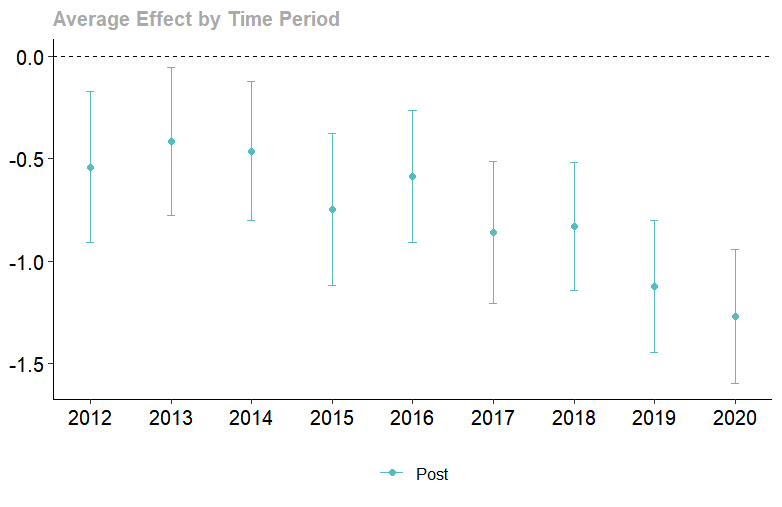
\includegraphics[width=0.85\textwidth]{Figuras/callaway_time.png}
\end{center}

\end{box_code}

\vspace{3mm}

\textbf{Qual é o  efeito médio do tratamento para cada ano adicional de
tratamento?}

\vspace{3mm}

Na análise anterior estamos agrupando todos os tratados no mesmo ano, incluindo efeitos de diferentes exposições ao tratamento. Por exemplo, no ano de 2018, temos grupos tratados por 1 período, outros por 3 períodos, e outro por 5 períodos. A média por ano agrupa todos esses grupos com diferentes tempos de tratamento. No entanto, uma questão frequentemente crucial em análises de políticas públicas é avaliar quanto cada período adicional de tratamento gera de efeito.

Assim, muitas vezes, desejamos estimar qual é o efeito médio do tratamento ao longo de diferentes períodos de tempo, como o de ser tratado por 1 período, por 2 períodos, e assim por diante. Para isso, construímos uma variável que representa a quantidade de períodos desde o tratamento, ou seja, $d = t - g$. Por exemplo, se estivermos no ano de 2016 e o grupo foi tratado pela primeira vez em 2012 ($g=2012$), estamos no quarto ano de tratamento, $d = 2016 - 2012 = 4$. Para calcular o efeito médio de ser tratado por 1 período, atribuiremos peso igual para todos os $ATT(g,t)$, onde $d=t-g=1$. Em outras palavras, consideraremos os $ATT(2012,2013)$, $ATT(2013,2014)$, e assim por diante, enquanto atribuímos peso 0 para todos os outros $ATTs$.

Para isso, basta agregarmos como \textit{'dynamic'} no pacote \textit{did}. 

\begin{box_code}

\begin{Shaded}
\begin{Highlighting}[]
\CommentTok{\#Teste Efeito longo prazo x curto prazo}

\NormalTok{att\_d }\OtherTok{=} \FunctionTok{aggte}\NormalTok{(ATT\_gt, }\AttributeTok{type =} \StringTok{\textquotesingle{}dynamic\textquotesingle{}}\NormalTok{)}

\FunctionTok{summary}\NormalTok{(att\_d)}
\end{Highlighting}
\end{Shaded}

\begin{verbatim}
## 
## Call:
## aggte(MP = ATT_gt, type = "dynamic")
## 
## Reference: Callaway, Brantly and Pedro H.C. Sant'Anna.  
## "Difference-in-Differences with Multiple Time Periods." 
## Journal of Econometrics, Vol. 225, No. 2, pp. 200-230, 2021. 
## <https://doi.org/10.1016/j.jeconom.2020.12.001>, 
## <https://arxiv.org/abs/1803.09015> 
## 
## 
## Overall summary of ATT's based on event-study/dynamic 
## aggregation:  
##      ATT    Std. Error     [ 95%  Conf. Int.]  
##  -1.0396         0.079    -1.1945     -0.8847 *
## 
## 
## Dynamic Effects:
##  Event time Estimate Std. Error [95% Simult.  Conf. Band]  
##          -6  -0.0262     0.1397     -0.4418      0.3895  
##          -5   0.0157     0.1544     -0.4439      0.4753  
##          -4   0.0670     0.1048     -0.2451      0.3790  
##          -3  -0.0416     0.1201     -0.3990      0.3159  
##          -2  -0.0576     0.1043     -0.3682      0.2529  
##          -1   0.0069     0.1053     -0.3064      0.3202  
##           0  -0.2760     0.0866     -0.5337     -0.0183 *
##           1  -0.4142     0.0838     -0.6635     -0.1649 *
##           2  -0.6720     0.0971     -0.9609     -0.3831 *
##           3  -0.9519     0.0976     -1.2424     -0.6614 *
##           4  -0.9949     0.1171     -1.3434     -0.6464 *
##           5  -1.1342     0.1377     -1.5441     -0.7243 *
##           6  -1.2616     0.1423     -1.6851     -0.8381 *
##           7  -1.7642     0.1925     -2.3371     -1.1914 *
##           8  -1.8876     0.1847     -2.4374     -1.3378 *
## ---
## Signif. codes: `*' confidence band does not cover 0
## 
## Control Group:  Never Treated,  Anticipation Periods:  0
## Estimation Method:  Doubly Robust
\end{verbatim}

\end{box_code}

Portanto, no ano da intervenção, em média, observamos um efeito de $-0.2760$ ponto percentual (p.p.). Um ano após o início da intervenção, o efeito foi de $-0.4142$ p.p., após 2 anos, de -0.6720 p.p., e assim por diante. Além disso, temos a média geral (simples) dos ATTs dinâmicos. No caso do nosso exemplo, $-1$ p.p.

Podemos plotar um gráfico diretamente através do pacote \textit{did}:

\begin{box_code}

\begin{Shaded}
\begin{Highlighting}[]
\CommentTok{\# Plotando gráfico efeito dinamico/event study}
\FunctionTok{ggdid}\NormalTok{(att\_d)}
\end{Highlighting}
\end{Shaded}

\begin{center}
    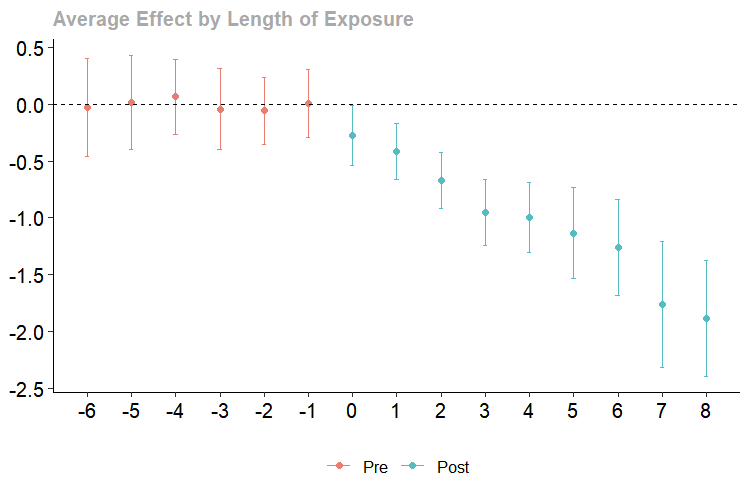
\includegraphics[width=0.85\textwidth]{Figuras/callaway_dynamic.png}
\end{center}

\end{box_code}

Este gráfico apresenta um método visual eficaz para avaliar tendências paralelas antes do tratamento (onde \(d = -1, -2, \ldots, -6\)). Por essa razão, é amplamente utilizado em muitos trabalhos científicos.


\subsection{\cite{de2020two}}

\subsubsection{Estimador}

A abordagem de \citet{de2020two} difere consideravelmente dos outros trabalhos anteriormente vistos, embora, essencialmente, esteja estimando um $ATT(g,t)$ específico. O problema do TWFE é que ponderamos erroneamente os ATTs, ou, por outra perspectiva, estamos aplicando DID 2x2 para todos os grupos e acabamos usando um grupo tratado como controle para outro grupo tratado.

Dessa forma, o estimador proposto por \citet{de2020two} irá calcular diferenças-em-diferenças 2 a 2 separadamente e depois reponderar de forma correta. A diferença será que, para cada período, utiliza-se como grupo tratado apenas os grupos que mudam de status tratamento naquele período, ou seja, aqueles que passam de tratado para controle ou de controle para tratado.

Considere o exemplo simples onde temos 3 períodos pós tratamento e 3 grupos de tratamento e, além disso, o tratamento é escalonado. Ou seja, $t \in \{0, 1,2, 3\}$ e $G = \{1,2,3\}$ e se $g\geq t$, todos do grupo $g$ são tratados em $t$. Na tabela abaixo, os controles em cada período serão identificados em verde, os tratados em vermelho e ``-" significa que aquele(s) grupo(s) não será(ão) usado(s). Além disso, uma outra mudança em relação a \cite{callaway2021difference} e \cite{sun2021estimating} é que as comparações dois a dois são feitas sempre entre $t$ e $t-1$. 


% Please add the following required packages to your document preamble:
% \usepackage[table,xcdraw]{xcolor}
% Beamer presentation requires \usepackage{colortbl} instead of \usepackage[table,xcdraw]{xcolor}
\begin{table}[!htp]
\centering
\begin{tabular}{|c|c|c|c|c|}
\hline
t\textbackslash{}g & $\infty$  & 1  & 2 & 3 \\ \hline
0                  &          &   &  &  \\ \hline
1                  & \textcolor{green}{\textbullet }& \textcolor{red}{\textbullet } & \textcolor{green}{\textbullet } & \textcolor{green}{\textbullet } \\
2                  & \textcolor{green}{\textbullet } & - & \textcolor{red}{\textbullet} & \textcolor{green}{\textbullet} \\
3                  & \textcolor{green}{\textbullet} & - & - & \textcolor{red}{\textbullet} \\
\hline
\end{tabular}
\end{table}

Diferente da literatura padrão de diferença-em-diferença escalonado, \citet{de2020two} possibilitam entradas e saídas do tratamento em qualquer período e em qualquer quantidade de vezes. Entretanto, isso fará com que precisemos ter algumas hipóteses adicionais que serão melhor estudadas na Seção \ref{subsec:char_hyp}. Uma delas é que em todos os períodos em que um grupo entrar no tratamento (ou seja, $d_{g,t-1} = 0$ e $d_{g,t}=1$), deve haver pelo menos um grupo que não é tratado naquele período e no período anterior (ou seja, $d_{g',t-1}=d_{g',t} = 0$). E, em todos os períodos em que um grupo deixar de ser tratado (ou seja, $d_{g,t-1}=1$ e $d_{g,t}=0$), deve haver pelo menos um grupo que é tratado naquele período e no período passado (ou seja, $d_{g',t} = d_{g',t-1}=1$).

Isso é necessário porque, no caso do grupo que passou a ser tratado, precisamos de pelo menos um grupo que não foi tratado nos dois períodos para servir como controle. Enquanto isso, no caso de um grupo que deixou de ser tratado, precisaremos de um grupo que é tratado nos dois períodos para ser seu controle. O sinal do efeito no segundo caso será invertido, pois estamos comparando sair do tratamento contra ficar. E é por isso que \citet{de2020two} dividem o estimador em dois componentes: $DID_{+,t}$ e $DID_{-,t}$, que seriam a diferença-em-diferenças padrão e a diferença-em-diferenças "invertida", isso é, multiplicada por  $-1$.

E, por fim, agregamos com pesos corretos cada DID, inclusive com peso negativo para o $DID_{-,t}$. Para construirmos o estimador, definamos:

\[
\begin{split}
    N_{d,d', t} = \sum_{g: d_{g,t} = d, d_{g,t-1} = d'} N_{g,t}
\end{split}
\]

$N_{d,d', t}$ é a quantidade de observações no grupo com $d \in \{0,1\}$ no período $t$ e $d' \in \{0,1\}$ no período $t-1$. Ou seja, $N_{0,0,t}$ é a quantidade de observações entre todos os grupos que não eram tratadas em $t-1$ continuaram não tratadas no período $t$. $N_{1,0,t}$ é a quantidade de observações em todos os grupos que passaram a ser tratadas em $t$, e assim por diante. 

Podemos definir, portanto:

\[
\begin{split}
    DID_{+,t} &= \sum_{g: d_{g,t} = 1, d_{g,t-1} = 0} \frac{N_{g,t}}{N_{1,0, t}} (Y_{g,t} - Y_{g,t-1}) - \sum_{g: d_{g,t} = d_{g,t-1} = 0} \frac{N_{g,t}}{N_{0,0,t}} (Y_{g,t} - Y_{g,t-1}) \\
    DID_{-,t} &= \sum_{g: d_{g,t} = d_{g,t-1} = 1} \frac{N_{g,t}}{N_{1,1, t}} (Y_{g,t} - Y_{g,t-1}) - \sum_{g: d_{g,t} = 1, d_{g,t-1} = 0} \frac{N_{g,t}}{N_{0,1,t}} (Y_{g,t} - Y_{g,t-1}) \\
\end{split}
\]

\noindent definamos $N_S = \sum_{(g;t):t\geq2, D_{g,t}\neq D_{g,t-1}} N_{g,t}$\footnote{$N_S$ é a quantidade total de unidades que mudam de status de tratamento em t.}. Nosso estimador, portanto, será:

\[
\begin{split}
    DID_{M} &= \sum_{t=2}^{T} \left[ \frac{N_{1,0,t}}{N_S} DID_{+,t} + \frac{N_{0,1,t}}{N_S} DID_{-,t} \right] 
\end{split}
\]

\noindent Veja que $DID_{M}$ é uma média ponderada pelo tamanho relativo de cada grupo em cada período. Isso funciona porque, a cada período, estamos fazendo um modelo de diferenças-em-diferenças para cada "tipo" de tratamento. Ou seja, estamos realizando DIDs 2x2 separadamente e em seguida os reponderando, em vez de os estimarmos de forma agregada, como no TWFE.

\subsubsection{Hipóteses} \label{subsec:char_hyp}

Entre os artigos da literatura, \cite{de2020two} é o que mais flexibiliza o tipo de tratamento ao longo do tempo e entre grupos. Para isso, são necessárias hipóteses um pouco mais fortes. Para mantermos a notação de \cite{de2020two}, replicaremos a numeração das hipóteses conforme o artigo. Entretanto, algumas hipóteses lá mencionadas são utilizadas apenas para provar o não viés do TWFE. Nesse caso, como não são necessárias para a consistência do $DID_M$, vamos omiti-las. 


\begin{boxB}
    \begin{enumerate}

        \item \textbf{HIPÓTESE 1 (Painel Balanceado de Grupos):} Para todo $(g,t) \in \{1,\ldots,G\} \times \{1,\ldots,T\}$, $N_{g,t} > 0$.

        \item \textbf{HIPÓTESE 2 (\textit{Sharp Design}):} Para todo $(g,t) \in \{1,\ldots,G\} \times \{1,\ldots,T\}$ e $i \in \{1,\ldots, N_{g,t}\}$, $D_{i,g,t} = D_{g,t}$.

        \item \textbf{HIPÓTESE 4 (Exogeneidade Forte):} Para todo $(g,t) \in \{1,\ldots,G\} \times \{2,\ldots,T\}$,
$$E\left(Y_{g,t}^{(0)} - Y_{g,t-1}^{(0)} | D_{g,1},\ldots, D_{g,T}\right) = E\left(Y_{g,t}^{(0)} - Y_{g,t-1}^{(0)}\right).$$

        \item \textbf{HIPÓTESE 5 (Tendências paralelas):} Para $t \geq 2$, $E(Y_{g,t}^{(0)} - Y_{g,t-1}^{(0)})$ não varia entre os grupos $g$.

        \item \textbf{HIPÓTESE 9 (Exogeneidade Forte para $Y(1)$):} Para todo $(g,t) \in \{1,\ldots,G\} \times \{2,\ldots,T\}$, 
$$E\left(Y_{g,t}^{(1)} - Y_{g,t-1}^{(1)} | D_{g,1},\ldots, D_{g,T}\right) = E\left(Y_{g,t}^{(1)} - Y_{g,t-1}^{(1)}\right).$$

        \item \textbf{HIPÓTESE 10 (Tendências paralelas para $Y(1)$):} Para $t \geq 2$, $E(Y_{g,t}^{(1)} - Y_{g,t-1}^{(1)})$ não varia entre os grupos $g$.

        \item \textbf{HIPÓTESE 11 (Existência de Grupos "Estáveis"):} Para todo $t \in \{2,\ldots,T\}$:
        \begin{enumerate}
            \item Se existe pelo menos um $g \in \{1,\ldots,G\}$ tal que $D_{g,t-1} = 0$ e $D_{g,t} = 1$, então existe pelo menos um $g' \neq g, g' \in \{1,\ldots,G\}$ tal que $D_{g',t-1} = D_{g',t} = 0$.
            \item Se existe pelo menos um $g \in \{1,\ldots,G\}$ tal que $D_{g,t-1} = 1$ e $D_{g,t} = 0$, então existe pelo menos um $g' \neq g, g' \in \{1,\ldots,G\}$ tal que $D_{g',t-1} = D_{g',t} = 1$.
        \end{enumerate}

        \item \textbf{HIPÓTESE 12 (Independência da Média entre o Resultado de um Grupo e os Tratamentos de Outros Grupos):} Para todos $g$ e $t$, $E(Y_{g,t}(0)|D) = E(Y_{g,t}(0)|D_g)$ e $E(Y_{g,t}(1)|D) = E(Y_{g,t}(1)|D_g)$.
        
                 
    \end{enumerate}
    \cite{de2020two}
\end{boxB}

A hipótese 1 garante que os grupos não ''sumam'' da base de dados durante o período analisado. Já a hipótese 2 garante que todos os indivíduos em $(g,t)$ terão o mesmo status de tratamento. Entretanto, \citet{de2020two} propõem um estimador consistente também quando essa hipótese é flexibilizada. %Por fim, a hipótese 3 implica que os resultados potenciais de um grupo são independentes dos potenciais resultados dos outros grupos. 
As hipóteses 1 e 2 estão presentes em todos os outros trabalhos da literatura, ainda que de forma não explícita.

A hipótese 4 e 5 são muito semelhantes às hipóteses de \citet{sun2021estimating}. Conjuntamente, elas afirmam que a tendência paralela deve ser independente do tratamento e igual pra todos os grupos. Isso implica que o momento em que um indivíduo será tratado não pode ser afetado por choques passados, por exemplo. Essa é uma das grandes diferenças em relação ao trabalho de \citet{callaway2021difference}. Perceba que não temos a restrição adicional de que as tendências paralelas devem ser constantes ao longo do tempo. A hipótese 5 e 10 impõem restrições de que as tendências paralelas devem ser constantes entre os grupos, tanto para o resultado potencial para o caso não tratado (5) quanto para o caso tratado (10). Ou seja, elas podem variar ao longo do tempo, mas não podem ser dependentes, em média, do tratamento ou variar ao longo dos grupos.

A hipótese 9 é essencialmente a mesma que a hipótese 4, porém aplicada ao resultado potencial em caso de tratamento. Ou seja, além do tratamento ser independente, em média, do resultado potencial de não tratamento, ele também deve ser independente para o resultado potencial caso seja tratado. Essa hipótese é mais forte que as hipóteses necessárias em \cite{callaway2021difference} e em \cite{sun2021estimating}. 

A hipótese 11 requer que para todo período em que haja um grupo que passa de não tratado para tratado, haja ao menos um grupo que não seja tratado nos dois períodos em questão. O mesmo vale para os períodos em que haja um grupo que deixou de ser tratado, ou seja, passou de tratado para não tratado. Neste caso, precisamos ter pelo menos um grupo que seja tratado no período em questão e no período anterior. Isso é necessário para garantirmos que em todos os períodos tenhamos grupos de controle. Por fim, a hipótese 12 implica que, condicional ao tratamento, os resultados potenciais dos grupos são independentes entre si.

\begin{boxaplicado}
\cite{diasfontes2024} investigam os efeitos da Reforma Psiquiátrica Brasileira de 2002, que introduziu os Centros de Atenção Psicossocial (CAPS) como alternativa comunitária ao modelo de internações hospitalares em psiquiatria. Como os CAPS foram implementados a nível municipal e de maneira gradual, os autores puderam usar um modelo de diferenças-em-diferenças escalonado usando o estimador de \cite{de2020two}.

O objetivo foi avaliar os impactos dessa política na prestação de cuidados de saúde mental, hospitalizações psiquiátricas, mortalidade, despesas públicas e indicadores sociais, como taxas de criminalidade.  A análise utilizou dados de 5.180 municípios brasileiros de 2002 a 2016, e foram examinados impactos em indicadores de saúde, finanças públicas e taxas de homicídios, com controles  para tendências prévias e características socioeconômicas locais.

Os CAPS foram abertos em cada município mediante pedido ao Governo Federal, a seu critério. Os primeiros CAPS (nos termos da reforma) foram abertos em 2002, e, até 2016, entre 50 a mais de 200 municípios receberam seu primeiro CAPS anualmente. Dessa forma, cada ano corresponde a um grupo de tratamento (conjunto de municípios que receberam um CAPS naquele ano). A apresentação dos resultados foi feita em formato de \textit{event study} (ATTs para $k$ períodos após o recebimento do tratamento), e ponderada pelo tamanho relativo de cada coorte. 

A criação dos CAPS aumentou a oferta de serviços ambulatoriais de saúde mental e reduziu hospitalizações psiquiátricas, especialmente de longa duração e entre pacientes com esquizofrenia. Apesar disso, a economia dos gastos com internações não compensou os custos do programa, gerando um impacto financeiro líquido negativo – ao contrário do que se propunha com a reforma. A política não reduziu significantemente a mortalidade por causas relacionadas à saúde mental e esteve associada a um aumento nas taxas de homicídios, possivelmente alinhado à hipótese de Penrose, que associa a redução de internações com maior exposição de pacientes vulneráveis à violência.

\end{boxaplicado}



\subsubsection{Código em R com exemplo}

Primeiro, vamos carregar a base de dados.

\begin{box_code}

    \begin{Shaded}
    \begin{Highlighting}[]
    \FunctionTok{rm}\NormalTok{(}\AttributeTok{list=}\FunctionTok{ls}\NormalTok{())}
    \FunctionTok{library}\NormalTok{(dplyr)}
    
    \NormalTok{df }\OtherTok{\textless{}{-}} \FunctionTok{read.csv}\NormalTok{(}\StringTok{"base\_stagger\_did.csv"}\NormalTok{)}
    
    \FunctionTok{head}\NormalTok{(df)}
    \end{Highlighting}
    \end{Shaded}

    \begin{verbatim}
    ##   id_estado id_municipio     setor  ano renda 
    ##           1         1001 ServiC'os 2011  55.9          
    ##           1         1001 ServiC'os 2012  60.0         
    ##           1         1001 ServiC'os 2013  65.0          
    ##           1         1001 ServiC'os 2014  81.0 
    ##           1         1001 ServiC'os 2015  78.0
    ##           1         1001 ServiC'os 2016  77.0
    ## escolaridade populacao         y d G Tt d_x_t
    ##          8.9    117002  9.804006 0 0  0     0
    ##          8.8    117510 11.145862 0 0  1     0
    ##          8.8    117754  5.578302 0 0  1     0
    ##          8.9    118655  4.967904 0 0  1     0
    ##          8.9    119788  4.748321 0 0  1     0
    ##          9.0    120792  5.564256 0 0  1     0
    
    \end{verbatim}

\end{box_code}

Em seguida, carregaremos o pacote \textit{DIDmultiplegt} para usarmos o modelo de \cite{de2020two} no R. 
\begin{box_code}

    \begin{Shaded}
    \begin{Highlighting}[]
    \FunctionTok{library}\NormalTok{(DIDmultiplegt)}
    \end{Highlighting}
    \end{Shaded}

\end{box_code}

Já com o pacote na memória, vamos usar a função \textit{did\_multiplegt}, que nos retornará o efeito médio de tratamento. Observamos que tivemos um efeito médio ao longo de toda a mostra de $-0,2499679$. Por padrão, esta função não calcula o desvio padrão do estimador.

\begin{box_code}

\begin{Shaded}

    \begin{Highlighting}[]
    \NormalTok{did }\OtherTok{=} \FunctionTok{did\_multiplegt}\NormalTok{(}
      \AttributeTok{df =}\NormalTok{ df,}
      \AttributeTok{Y =} \StringTok{"y"}\NormalTok{,}
      \AttributeTok{G =} \StringTok{"G"}\NormalTok{,}
      \AttributeTok{T =} \StringTok{"ano"}\NormalTok{,}
      \AttributeTok{D =} \StringTok{"d\_x\_t"}\NormalTok{,}
      \AttributeTok{controls =} \FunctionTok{c}\NormalTok{(}\StringTok{"renda"}\NormalTok{, }\StringTok{"escolaridade"}\NormalTok{, }\StringTok{"populacao"}\NormalTok{),}
      \AttributeTok{average\_effect =}\NormalTok{ T}
    \NormalTok{)}
    
    \NormalTok{did}
    \end{Highlighting}
    \end{Shaded}

    \begin{verbatim}
    ## $effect
    ##  treatment 
    ## -0.2499679 
    ## 
    ## $N_effect
    ## [1] 3660
    ## 
    ## $N_switchers_effect
    ## [1] 720
    \end{verbatim}
    

\end{box_code}

Agora, se quisermos o efeito dinâmico como fizemos com \citet{callaway2021difference, sun2021estimating}, devemos igualar o parâmetro \texttt{dynamic} ao número de períodos pós tratamento utilizados. No nosso caso, temos 8 períodos pós tratamento, então \texttt{dynamic} = 8. Além disso, para calcularmos os desvios padrões, precisamos definir \texttt{brep}, que é o número de replicações do \textit{bootstrap}. O ideal seria utilizar um número alto de replicações, algo em torno de 1000 ou mais. Para fins de exemplificação, no entanto, usaremos \texttt{brep} = 2, pois a implementação do software não funciona muito bem e não é eficiente.

\begin{box_code}

\begin{Shaded}
\begin{Highlighting}[]
\NormalTok{did }\OtherTok{=} \FunctionTok{did\_multiplegt}\NormalTok{(}
  \AttributeTok{df =}\NormalTok{ df,}
  \AttributeTok{Y =} \StringTok{"y"}\NormalTok{,}
  \AttributeTok{G =} \StringTok{"G"}\NormalTok{,}
  \AttributeTok{T =} \StringTok{"ano"}\NormalTok{,}
  \AttributeTok{D =} \StringTok{"d\_x\_t"}\NormalTok{,}
  \AttributeTok{controls =} \FunctionTok{c}\NormalTok{(}\StringTok{"renda"}\NormalTok{, }\StringTok{"escolaridade"}\NormalTok{, }\StringTok{"populacao"}\NormalTok{),}
  \AttributeTok{placebo =} \DecValTok{6}\NormalTok{,}
  \AttributeTok{dynamic =} \DecValTok{8}\NormalTok{,}
  \AttributeTok{brep =} \DecValTok{2}
\NormalTok{)}
\end{Highlighting}
\end{Shaded}

\begin{center}
    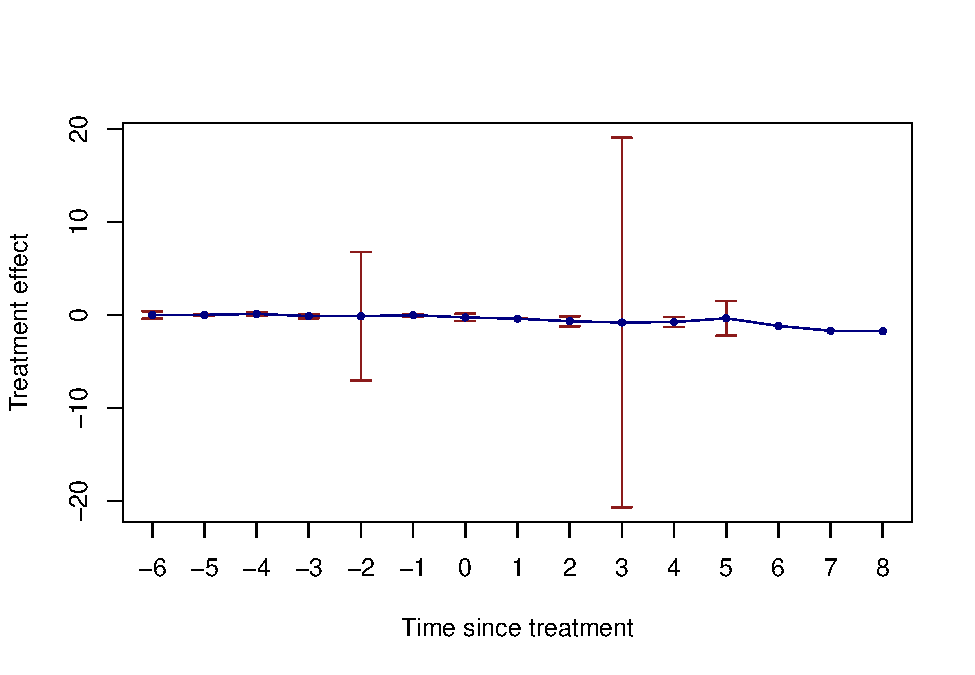
\includegraphics[width=0.85\textwidth]{Figuras/chas.pdf}
\end{center}

\end{box_code}

\subsection{\cite{borusyak2024revisiting}}

\subsubsection{Estimador}

Novamente, o objetivo será estimar de forma consistente o $ATT(g,t)$ condicional definido por:

\[
ATT(g,t) = E[y_{it}(g) - y_{it}(0) | X, d=g]
\]

e depois calculamos a média ponderada dos $ATT(g,t)$ que for mais conveniente para a nossa análise, como fizemos em \citet{callaway2021difference}.

\citet{borusyak2024revisiting} segue pelo mesmo caminho. Entretanto, propõe duas formas alternativas de estimação, sendo que uma requer hipóteses muito mais restritivas, mas é o mais eficiente entre todos os estimadores lineares. Como ambos são, de certa forma, distintos entre si, iremos subdividir esta seção em 2 subseções: \textit{Estimação Eficiente}, onde mostraremos o estimador eficiente porém mais restritivo, e \textit{Estimador de Imputação}, onde mostraremos o principal estimador em \citet{borusyak2024revisiting}.

\vspace{5mm}

{\large \textbf{\textit{Estimação Eficiente}}}

\vspace{2.5mm}

O grande problema dos modelos de diferença-em-diferença escalonado usando TWFE é que a heterogeneidade dos efeitos do tratamento gerará um estimador que será uma média ponderada dos $ATT(g,t)$ com pesos pouco informativos ou, ainda, negativos.

Para resolver o problema, \cite{borusyak2024revisiting} propõem assumirmos uma estrutura paramétrica para a heterogeneidade do tratamento. Ou seja, assumiremos que a forma da heterogeneidade do efeito do tratamento é conhecida e estimaremos um TWFE impondo essa estrutura paramétrica \textbf{conhecida}. 

Caso fossemos estimar um TWFE padrão, estimaríamos:

$$ y_{it} = \tilde{\alpha}_i + \tilde{\gamma}_t + \tilde{\tau} D_{it} + \varepsilon_{it} $$

\noindent onde $D_{it}$ é uma indicadora que é igual a 1 se o individuo $i$ é tratado no período $t$ e zero caso contrário. 

Novamente, o problema vem da heterogeneidade em $\tilde{\tau}$. Portanto, vamos assumir que a heterogeneidade pode ser descrita como:

$$ \tau = \Gamma\theta$$

\noindent onde $\theta$ é um vetor $(N_1 - M) \times 1$ e $\Gamma$ uma matriz $N_1 \times (N_1 - M)$ com \textit{rank} completo e \textbf{conhecida}. Nesse caso, $\theta$ é desconhecido e contém nossos parâmetros de interesse, que são os diferentes efeitos de tratamento. $N_1$,\footnote{Na notação de \cite{borusyak2024revisiting} $N_1 = |\Omega_1|, \Omega_1 = \{ it \in \Omega | D_{it} = 1\} $. Isto é, $\Omega_1$ representa o conjunto de observações indivíduo-tempo em que o indivíduo é tratado (e $\Omega$ o conjunto de todas as observações), e $N_1$ é o número de elementos desse conjunto.} representa o total de observações tratadas (e, assim, o número máximo de efeitos de tratamento distintos possíveis), e $M$ o número de restrições sobre os parâmetros. De forma que $N_1 - M$ é o número de parâmetros livres a serem estimados. Por exemplo, se assumirmos que o efeito é constante entre todos os grupos e períodos ($ATT(g,t) = ATT(g',t') = \theta_1$ para todo $g, g'$ e para todo $t \geq g$ e $t' \geq g'$), então, $N_1 - M = 1$, $\theta = \theta_1$ e $\Gamma = \underbrace{(1, \dots, 1)'}_{N_1\text{ vezes}}$.

Apesar de podermos escrever diversos tipos de heterogeneidade com essa versão paramétrica, nós precisamos assumir que a heterogeneidade é constante em alguma dimensão e, principalmente, que ela é conhecida. Assumindo isso, podemos rodar o MQO restrito a essa heterogeneidade:

\begin{equation}\label{eq:borusyak_TWFE}
    y_{it} = \alpha_i + \gamma_t + D_{it} \Gamma'_{it} \theta + \varepsilon_{it}
\end{equation}

\noindent onde $\Gamma_{it}$ é conhecido. Isso é equivalente a saturar o modelo com indicadoras para cada subgrupo onde o tratamento é heterogêneo.

\citet{borusyak2024revisiting} mostra que esse estimador será o mais eficiente entre todos os estimadores lineares para $\theta$. Entretanto, se a especificação escolhida para a heterogeneidade for incorreta, o estimador será inconsistente. Portanto, ele argumenta que a menos que exista uma justificativa muito forte ex-ante de que a heterogeneidade terá uma forma exata, é preferível usar o estimador de imputação, mesmo que não seja o mais eficiente.

\vspace{5mm}

{\large \textbf{\textit{Estimador de Imputação}}}

\vspace{2.5mm}

Ao estimar o $ATT(g,t)$, o que não se observa é $y_{it}(0)$ para quem é tratado no período $t$. O método de imputação passará por estimar $y_{it}(0)$ consistentemente e utilizarmos essa estimativa para estimar o $ATT(g,t)$.

Para isso, utilizaremos a hipótese de que $E[y_{it}(0)] = A'_{it} \lambda_i + X'_{it}\gamma$. Podemos escrever:

\begin{equation}\label{eq:borusyak}
    y_{it}(0) = A'_{it} \lambda_i + X'_{it}\gamma + \varepsilon_{it}
\end{equation}

\noindent onde $A_{it}$ e $X_{it}$ são vetores observáveis e conhecidos. Veja que se $A_{it} = 1$ para todo $i$ e $t$, temos o efeito fixo de indivíduo e se $X_{it}$ contiver uma indicadora para cada período, temos o efeito fixo de tempo. Além disso, $A'_{it}$ pode conter as covariáveis interagidas com uma indicadora para cada grupo, de forma que a Hipótese 1 da próxima seção torna-se muito próxima da hipótese de tendências paralelas que podem variar entre grupos.

Defina $\Omega_0$ como o conjunto de todos as observações não tratadas e $\Omega_1$ o conjunto de todas observações tratadas.

\begin{enumerate}
    \item Estimamos $\hat{\lambda}_i$ e $\hat{\gamma}$ via equação \ref{eq:borusyak} por MQO em todas as observações não tratadas (i.e., $it \in \Omega_0$)

    \item Para toda observação tratada ($it \in \Omega_1$), calculamos:

    $$\hat{y}_{it}(0) = A'_{it} \hat{\lambda}_i + X^\prime_{it} \hat{\gamma}$$
    
    \item Calculamos o efeito do tratamento para cada observação tratada ($it \in \Omega_1$):

    $$ \hat{\tau}_{it} = y_{it} - \hat{y}_{it}(0)  $$ 

    \item E, por fim, agregamos os efeitos com algum peso arbitrário tal que $\sum_{it} w_{it} = 1$ e $\forall i,t, w_{it} \geq 0$. Ou seja:

    $$ \hat{\tau} = \sum_{it} w_{it} \hat{\tau}_{it} $$

\end{enumerate}


Esse método calcula, indiretamente, algo muito semelhante ao $ATT(g,t)$. É como se calculássemos cada um dos $ATT(g,t)$ ao reponderar os $\hat{\tau}_{it}$ por $w_{it}/\sum_{i \in g} w_{it}$ para cada observação no grupo $g$. Se assumirmos que o peso é igual para todos os indivíduos do mesmo grupo em cada período, acabamos por estimar exatamente igual a \citet{callaway2021difference}, uma média ponderada dos $ATT(g,t)$.

\vspace{5mm}

{\large \textbf{\textit{Inferência}}}

\vspace{2.5mm}

Para a inferência, \cite{borusyak2024revisiting} mostra que é impossível estimarmos consistentemente a variância paramétrica de $\hat{\tau}_{it}$ e, por consequência, de $\hat{\tau}$. Entretanto, defina $v_{it}$ os pesos relativos para cada observação $(i,t)$ tal que $\hat{\tau} = \sum_{it} v_{it} y_{it}$,\footnote{Para qualquer vetor de pesos $w$ tal que $\hat{\tau} = \sum_{it} w_{it} \hat{\tau}_{it}$, existe um vetor de pesos $v_{it}$ tal que $\hat{\tau} = \sum_{it} v_{it} y_{it}$. Veja \cite{borusyak2024revisiting}, seção 4.2 para mais detalhes.} sob as hipóteses da próxima seção, a variância dada por:

\begin{equation}\label{eq:var_borusyak}
    \hat{\sigma}_w^2 = \sum_{i} \left( \sum_{t;it \in \Omega_1} v_{it} \tilde{\varepsilon}_{it} \right)^2, \text{ } \tilde{\varepsilon}_{it} = y_{it} - A_{it}^\prime \hat{\lambda}_i - X_{it}^\prime \hat{\lambda} - D_{it} \hat{\tau}_{it}
\end{equation}

\noindent  é uma estimativa conservadora da variância assintótica. Isto é, ela convergirá para uma variância maior ou igual à variância verdadeira. Assim, se rejeitarmos a hipótese nula de efeito zero, isso será uma evidência ainda mais forte de que o efeito é não nulo. Em contrapartida, nosso poder será menor. 


\subsubsection{Hipóteses}

\begin{boxB}
    \begin{enumerate}

    \item \textbf{HIPÓTESE 1 (Modelo Geral de $Y(0)$):} Para todo $it \in \Omega_0$,
    $$E\left[Y_{it}^{(0)}\right] = A'_{it} \lambda_i + X'_{it} \gamma$$
    \noindent onde $\lambda_i$ é um vetor de parâmetros não-observados específicos do indivíduo, $\delta$ é um vetor de parâmetros não-observados associados a covariáveis comuns, e $A_{it}$ e $X_{it}$ são vetores conhecidos e não-estocásticos.

    \item \textbf{HIPÓTESE 2 (No-anticipation effects):} $Y_{it} = Y_{it}(0)$ para todo $it \in \Omega_0$

    \item \textbf{HIPÓTESE 3 (Model of causal effects):} $\tau = \Gamma\theta$ onde $\theta$ é um vetor de parâmetros desconhecidos de dimensão $(N_1 - M) \times 1$ e $\Gamma$ é uma matriz conhecida de dimensão $N_1 \times (N_1 - M)$ de posto completo.
   
    \item \textbf{HIPÓTESE 5 (Termos de Erro com Clusters):} Os termos de erro $\epsilon_{it}$ são independentes entre as unidades $i$ e têm variância limitada, $Var[\epsilon_{it}] \leq \bar{\sigma}^2$ para $i,t \in \mathbb{N}$ uniformemente.

    \item \textbf{HIPÓTESE 6 (Condição de Herfindahl):} Ao longo da sequência assintótica, $v^2_H \equiv \sum_{it \in \mathbb{N}} |v_{it}|^2 \rightarrow 0$, para os pesos $v_{it}$ no estimador linear não viesado $\hat{\tau}_w = \sum_{it \in \mathbb{N}} v_{it} Y_{it}$.

    \end{enumerate}
    \citep{borusyak2024revisiting}
\end{boxB}

A princípio, as Hipóteses 1 e 3 podem parecer mais restritivas que as hipóteses em \cite{sun2021estimating}, \cite{callaway2021difference} e \cite{de2020two} por assumir uma forma paramétrica para o resultado potencial em caso de não tratamento. Entretanto, essa forma funcional é muito geral (abarcando o modelo TWFE, ou seja, a hipótese de tendências paralelas). Além disso, escolhendo corretamente $A_{it}$ e $X_{it}$, podemos permitir uma hipótese de tendências paralelas condicionais menos restritivas do que precisamos em \cite{sun2021estimating} e  \cite{de2020two}. Não é necessário assumir homogeneidade delas em relação às covariadas, i.e, não é necessário que $\mathbf{E[y_{it}(\infty) - y_{i0}(\infty) | G=g, X] = E[y_{it}(\infty) - y_{i0}(\infty)|G=g]}$.

A hipótese 2 é a hipótese padrão de não antecipação e podemos relaxá-la desde que tenhamos um número suficientemente grande de observações não tratadas. 

As Hipóteses 5 e 6 são necessárias para a inferência sobre o estimador $\tau$. Elas garantem que a distribuição assintótica dele será normal e que podemos construir estimadores conservadores para a variância. A maior restrição imposta é que as observações devem ser independentes entre os indivíduos, mesmo dentro do mesmo grupo, e que a norma do vetor de pesos deve convergir para zero. Essa última hipótese é semelhante à hipótese implícita em \citet{sun2021estimating}, onde o tamanho de todos os grupos deve aumentar quando $N$ aumenta.

\subsubsection{Código em R com exemplo}

Vamos construir nosso próprio código para rodarmos o modelo proposto por \cite{borusyak2024revisiting}.\footnote{Poderíamos utilizar o pacote \textit{didimputation} no R. Entretanto, apesar de abarcar os modelos com escalonamento no tratamento, ele atualmente (julho/2024) funciona com muitos erros nessas ocasiões.} Primeiramente, vamos carregar a base de dados do exemplo trabalhado até aqui.


\begin{box_code}

\begin{Shaded}
\begin{Highlighting}[]
\FunctionTok{rm}\NormalTok{(}\AttributeTok{list=}\FunctionTok{ls}\NormalTok{())}
\FunctionTok{library}\NormalTok{(dplyr)}

\NormalTok{df }\OtherTok{\textless{}{-}} \FunctionTok{read.csv}\NormalTok{(}\StringTok{"base\_stagger\_did.csv"}\NormalTok{)}

\FunctionTok{head}\NormalTok{(df)}
\end{Highlighting}
\end{Shaded}

\begin{verbatim}
##   id_estado id_municipio     setor  ano renda  y
## 1         1         1001 ServiC'os 2011  55.9  8.9    
## 2         1         1001 ServiC'os 2012  60.0  8.8    
## 3         1         1001 ServiC'os 2013  65.0  8.8    
## 4         1         1001 ServiC'os 2014  81.0  8.9    
## 5         1         1001 ServiC'os 2015  78.0  8.9    
## 6         1         1001 ServiC'os 2016  77.0  9.0    
##   escolaridade   populacao    d G Tt d_x_t
## 1       117002    9.804006    0 0  0     0
## 2       117510   11.145862    0 0  1     0
## 3       117754    5.578302    0 0  1     0
## 4       118655    4.967904    0 0  1     0
## 5       119788    4.748321    0 0  1     0
## 6       120792    5.564256    0 0  1     0
\end{verbatim}


\end{box_code}

Agora seguiremos cada um dos passos para construir o estimador de imputação. 

\begin{enumerate}
    \item Estimamos $\hat{\lambda}_i$ e $\hat{\gamma}$ via equação \ref{eq:borusyak} por MQO em todos as observações não tratadas (i.e., $it \in \Omega_0$).
\end{enumerate}

No nosso caso, a especificação conterá efeitos fixos de tempo, indivíduo e as covariadas escolaridade e população. Logo, estimaremos, com todos os indivíduos não tratados ($i \in \Omega_0$):

\begin{equation*}
     y_{it}(0) = \alpha_g + \delta_t + \gamma_1 escolaridade_{it} + \gamma_2 populacao_{it} + \varepsilon_{it}
\end{equation*}

Vamos então filtrar a base para manter apenas os não tratados e chamá-la de \textit{df0}:

\begin{box_code}

\begin{Shaded}
\begin{Highlighting}[]
    \NormalTok{df}\SpecialCharTok{$}\NormalTok{d\_x\_t }\OtherTok{=} \FunctionTok{ifelse}\NormalTok{(df}\SpecialCharTok{$}\NormalTok{ano }\SpecialCharTok{\textless{}=}\NormalTok{ df}\SpecialCharTok{$}\NormalTok{G }\SpecialCharTok{|}\NormalTok{ df}\SpecialCharTok{$}\NormalTok{G }\SpecialCharTok{==} \DecValTok{0}\NormalTok{, }\DecValTok{0}\NormalTok{, }\DecValTok{1}\NormalTok{)}
    
    \NormalTok{df0 }\OtherTok{=}\NormalTok{ df[df}\SpecialCharTok{$}\NormalTok{d\_x\_t }\SpecialCharTok{==} \DecValTok{0}\NormalTok{,]}
\end{Highlighting}
\end{Shaded}

\end{box_code}

Agora, vamos estimar a equação acima por MQO:

\begin{box_code}

\begin{Shaded}
\begin{Highlighting}[]
    \NormalTok{reg0 }\OtherTok{=} \FunctionTok{lm}\NormalTok{(y }\SpecialCharTok{\textasciitilde{}} \FunctionTok{as.factor}\NormalTok{(ano) }\SpecialCharTok{+} \FunctionTok{as.factor}\NormalTok{(G) }
                    \SpecialCharTok{+}\NormalTok{ escolaridade }\SpecialCharTok{+}\NormalTok{ populacao, }
              \AttributeTok{data =}\NormalTok{ df0)}
    
    \FunctionTok{library}\NormalTok{(stargazer)}
    \FunctionTok{stargazer}\NormalTok{(reg0, }\AttributeTok{title =} \StringTok{"Passo 1"}\NormalTok{)}
\end{Highlighting}
\end{Shaded}

\begingroup
    \fontsize{8pt}{12pt}\selectfont
    \begin{center}
    \caption{Modelo y(0) para imputation} \\
    \begin{tabular}{@{\extracolsep{5pt}}lc} 
    \\[-1.8ex]\hline 
    \hline \\[-1.8ex] 
     & \multicolumn{1}{c}{\textit{Dependent variable:}} \\ 
    \cline{2-2} 
    \\[-1.8ex] & y \\ 
    \hline \\[-1.8ex] 
     as.factor(ano)2012 & $-$1.220$^{***}$ \\ 
      & (0.059) \\ 
     as.factor(ano)2013 & $-$2.552$^{***}$ \\ 
      & (0.064) \\ 
     as.factor(ano)2014 & $-$3.751$^{***}$ \\ 
      & (0.064) \\ 
     as.factor(ano)2015 & $-$4.937$^{***}$ \\ 
      & (0.067) \\ 
     as.factor(ano)2016 & $-$6.289$^{***}$ \\ 
      & (0.067) \\ 
     as.factor(ano)2017 & $-$7.546$^{***}$ \\ 
      & (0.072) \\ 
     as.factor(ano)2018 & $-$8.841$^{***}$ \\ 
      & (0.073) \\ 
     as.factor(ano)2019 & $-$9.944$^{***}$ \\ 
      & (0.081) \\ 
     as.factor(ano)2020 & $-$11.208$^{***}$ \\ 
      & (0.081) \\ 
     as.factor(G)2012 & 6.372$^{***}$ \\ 
      & (0.076) \\ 
     as.factor(G)2014 & 6.166$^{***}$ \\ 
      & (0.072) \\ 
     as.factor(G)2016 & 6.102$^{***}$ \\ 
      & (0.051) \\ 
     as.factor(G)2018 & 5.985$^{***}$ \\ 
      & (0.045) \\ 
     escolaridade & $-$0.062$^{***}$ \\ 
      & (0.016) \\ 
     populacao & $-$0.00000 \\ 
      & (0.00000) \\ 
     Constant & 10.568$^{***}$ \\ 
      & (0.146) \\ 
    \hline \\[-1.8ex] 
    Observations & 8,280 \\ 
    R$^{2}$ & 0.933 \\ 
    Adjusted R$^{2}$ & 0.932 \\ 
    Residual Std. Error & 1.437 (df = 8264) \\ 
    F Statistic & 7,615.220$^{***}$ (df = 15; 8264) \\ 
    \hline 
    \hline \\[-1.8ex] 
    \textit{Note:}  & \multicolumn{1}{r}{$^{*}$p$<$0.1; $^{**}$p$<$0.05; $^{***}$p$<$0.01} \\ 
    \end{tabular} 
    \end{center}
 \endgroup

\end{box_code}

\begin{enumerate}
    \setcounter{enumi}{1}
   \item Para toda observação tratada ($it \in \Omega_1$), calculamos:

    $$\hat{y}_{it}(0) = A'_{it} \hat{\lambda}_i + X^\prime_{it} \hat{\gamma}$$
\end{enumerate}

\begin{box_code}

\begin{Shaded}
\begin{Highlighting}[]
    \CommentTok{\#Calculando y0 com o modelo anterior}
    \NormalTok{df}\SpecialCharTok{$}\NormalTok{y0\_hat }\OtherTok{=} \FunctionTok{predict}\NormalTok{(reg0, df)}
    
\end{Highlighting}
\end{Shaded}

\end{box_code}

\begin{enumerate}
    \setcounter{enumi}{2}
     \item Calculamos o efeito do tratamento para cada observação tratada ($it \in \Omega_1$):

    $$ \hat{\tau}_{it} = y_{it} - \hat{y}_{it}(0)  $$ 
\end{enumerate}

\begin{box_code}

\begin{Shaded}
\begin{Highlighting}[]
    \CommentTok{\# Calculando Tau via imputation}
    \NormalTok{df}\SpecialCharTok{$}\NormalTok{tau }\OtherTok{=} \DecValTok{0}
    \NormalTok{df[df}\SpecialCharTok{$}\NormalTok{d\_x\_t}\SpecialCharTok{==}\DecValTok{1}\NormalTok{, }\StringTok{\textquotesingle{}tau\textquotesingle{}}\NormalTok{] }\OtherTok{=}\NormalTok{ df[df}\SpecialCharTok{$}\NormalTok{d\_x\_t}\SpecialCharTok{==}\DecValTok{1}\NormalTok{, }\StringTok{\textquotesingle{}y\textquotesingle{}}\NormalTok{] }
                                \SpecialCharTok{{-}}\NormalTok{ df[df}\SpecialCharTok{$}\NormalTok{d\_x\_t}\SpecialCharTok{==}\DecValTok{1}\NormalTok{, }\StringTok{\textquotesingle{}y0\_hat\textquotesingle{}}\NormalTok{]}
    \end{Highlighting}
\end{Shaded}

\end{box_code}

Por fim, vamos ao passo 4. Juntamente, iremos calcular a variância proposta por \cite{borusyak2024revisiting}. Para saber mais da implementação, consultar o capítulo 4.3 e as proporisções 3 e 4 do apêndice de \cite{borusyak2024revisiting}.

\begin{enumerate}
    \setcounter{enumi}{3}
     \item E, por fim, agregaremos os efeitos com algum vetor de pesos arbitrário tal que $\sum_{it} w_{it} = 1$ e $\forall i,t, w_{it} \geq 0$. Ou seja:

        $$ \hat{\tau} = \sum_{it} w_{it} \hat{\tau}_{it} $$
\end{enumerate}

\begin{box_code}

    \begin{Shaded}
    \begin{Highlighting}[]
    \NormalTok{v0 }\OtherTok{\textless{}{-}} \ControlFlowTok{function}\NormalTok{(Z0, Z1, w)\{}
      
      \ControlFlowTok{if}\NormalTok{(}\FunctionTok{dim}\NormalTok{(Z0)[}\DecValTok{2}\NormalTok{] }\SpecialCharTok{!=} \FunctionTok{dim}\NormalTok{(Z1)[}\DecValTok{2}\NormalTok{]) \{}
        \FunctionTok{print}\NormalTok{(}\StringTok{\textquotesingle{}ERROR: Z0 e Z1 precisam ter o mesmo número}
        \StringTok{\textquotesingle{}de colunas.\textquotesingle{}}\NormalTok{)}
        \FunctionTok{return}\NormalTok{(}\StringTok{\textquotesingle{}\textquotesingle{}}\NormalTok{)}
    \NormalTok{  \}}
    
      \FunctionTok{dim}\NormalTok{(Z0 }\SpecialCharTok{\%*\%} \FunctionTok{solve}\NormalTok{(}\FunctionTok{t}\NormalTok{(Z0) }\SpecialCharTok{\%*\%}\NormalTok{ Z0))}
      
    \NormalTok{  v0 }\OtherTok{=} \SpecialCharTok{{-}}\NormalTok{ Z0 }\SpecialCharTok{\%*\%} \FunctionTok{solve}\NormalTok{(}\FunctionTok{t}\NormalTok{(Z0) }\SpecialCharTok{\%*\%}\NormalTok{ Z0) }\SpecialCharTok{\%*\%} \FunctionTok{t}\NormalTok{(Z1) }\SpecialCharTok{\%*\%} \FunctionTok{t}\NormalTok{(w)}
      \FunctionTok{return}\NormalTok{(v0)}

    \end{Highlighting}
    \end{Shaded}
      
    \begin{Shaded}
    \begin{Highlighting}[]
    
    \NormalTok{summarize\_tau }\OtherTok{\textless{}{-}} \ControlFlowTok{function}\NormalTok{(df, id\_name, G\_name, D\_name, }
                \NormalTok{formula, }\AttributeTok{restrict =} \ConstantTok{FALSE}\NormalTok{)\{}
      
      \FunctionTok{library}\NormalTok{(dplyr)}
    \NormalTok{  names\_var }\OtherTok{=} \FunctionTok{names}\NormalTok{(df)}
    
      \ControlFlowTok{for}\NormalTok{ (var }\ControlFlowTok{in} \FunctionTok{c}\NormalTok{(}\StringTok{\textquotesingle{}tau\textquotesingle{}}\NormalTok{, id\_name, G\_name, D\_name))\{}
        \ControlFlowTok{if}\NormalTok{(}\SpecialCharTok{!}\NormalTok{var }\SpecialCharTok{\%in\%}\NormalTok{ names\_var)\{}
          \FunctionTok{print}\NormalTok{(}\FunctionTok{c}\NormalTok{(}\StringTok{\textquotesingle{}ERRO: df precisa conter\textquotesingle{}}\NormalTok{, var))}
          \FunctionTok{return}\NormalTok{(}\StringTok{\textquotesingle{}\textquotesingle{}}\NormalTok{)}
    \NormalTok{    \}}
    \NormalTok{  \}}
      
    \NormalTok{  df}\SpecialCharTok{$}\NormalTok{G   }\OtherTok{=}\NormalTok{ df[,G\_name]}
    \NormalTok{  df}\SpecialCharTok{$}\NormalTok{id  }\OtherTok{=}\NormalTok{ df[,id\_name]}
    \NormalTok{  df}\SpecialCharTok{$}\NormalTok{D   }\OtherTok{=}\NormalTok{ df[,D\_name]}
      
    \NormalTok{  df1 }\OtherTok{=}\NormalTok{ df[df}\SpecialCharTok{$}\NormalTok{D}\SpecialCharTok{==}\DecValTok{1}\NormalTok{,]}
    \NormalTok{  df0 }\OtherTok{=}\NormalTok{ df[df}\SpecialCharTok{$}\NormalTok{D}\SpecialCharTok{==}\DecValTok{0}\NormalTok{,]}
      
      \CommentTok{\# Calculando Tau}
    \NormalTok{  df1}\SpecialCharTok{$}\NormalTok{w }\OtherTok{=} \FunctionTok{rep}\NormalTok{(}\DecValTok{1}\SpecialCharTok{/}\FunctionTok{length}\NormalTok{(df1}\SpecialCharTok{$}\NormalTok{tau), }\FunctionTok{length}\NormalTok{(df1}\SpecialCharTok{$}\NormalTok{tau))}
    \NormalTok{  w }\OtherTok{=} \FunctionTok{matrix}\NormalTok{(df1}\SpecialCharTok{$}\NormalTok{w, }\AttributeTok{nrow =} \DecValTok{1}\NormalTok{)}
    \NormalTok{  tau\_it }\OtherTok{=} \FunctionTok{matrix}\NormalTok{(df1}\SpecialCharTok{$}\NormalTok{tau, }\AttributeTok{ncol =} \DecValTok{1}\NormalTok{)}
      
    \NormalTok{  TAU }\OtherTok{=}\NormalTok{ w }\SpecialCharTok{\%*\%}\NormalTok{ tau\_it}

    \end{Highlighting}
    \end{Shaded}
      
    \begin{Shaded}
    \begin{Highlighting}[]
      
      \CommentTok{\#Calculando variância de Tau}
      
      \ControlFlowTok{if}\NormalTok{(restrict)\{}
        \CommentTok{\#Calculating tau\_g}
    \NormalTok{    df\_sum }\OtherTok{\textless{}{-}}\NormalTok{ df1 }\SpecialCharTok{\%\textgreater{}\%} \FunctionTok{group\_by}\NormalTok{(id, G) }\SpecialCharTok{\%\textgreater{}\%} 
                          \FunctionTok{summarise}\NormalTok{(}\AttributeTok{w =} \FunctionTok{sum}\NormalTok{(w),}
                                    \AttributeTok{wtau =} \FunctionTok{sum}\NormalTok{(w}\SpecialCharTok{*}\NormalTok{tau))}
        
    \NormalTok{    df\_g }\OtherTok{\textless{}{-}}\NormalTok{ df\_sum }\SpecialCharTok{\%\textgreater{}\%} \FunctionTok{group\_by}\NormalTok{(G) }\SpecialCharTok{\%\textgreater{}\%}
                           \FunctionTok{summarise}\NormalTok{(}\AttributeTok{numerador =} \FunctionTok{sum}\NormalTok{(w}\SpecialCharTok{*}\NormalTok{wtau),}
                                     \AttributeTok{denominador =} \FunctionTok{sum}\NormalTok{(w}\SpecialCharTok{\^{}}\DecValTok{2}\NormalTok{))}
        
    \NormalTok{    df\_g}\SpecialCharTok{$}\NormalTok{tau\_g }\OtherTok{=}\NormalTok{ df\_g}\SpecialCharTok{$}\NormalTok{numerador}\SpecialCharTok{/}\NormalTok{df\_g}\SpecialCharTok{$}\NormalTok{denominador}
        
    \NormalTok{    df\_res }\OtherTok{=} \FunctionTok{merge}\NormalTok{(df, df\_g[,}\FunctionTok{c}\NormalTok{(}\StringTok{\textquotesingle{}G\textquotesingle{}}\NormalTok{, }\StringTok{\textquotesingle{}tau\_g\textquotesingle{}}\NormalTok{)], }\AttributeTok{by =} \StringTok{\textquotesingle{}G\textquotesingle{}}\NormalTok{, }
                        \AttributeTok{all.x =}\NormalTok{ T)}
    \NormalTok{    df\_res[}\FunctionTok{is.na}\NormalTok{(df\_res}\SpecialCharTok{$}\NormalTok{tau\_g), }\StringTok{\textquotesingle{}tau\_g\textquotesingle{}}\NormalTok{] }\OtherTok{=} \DecValTok{0}
    \NormalTok{    df\_res}\SpecialCharTok{$}\NormalTok{res }\OtherTok{=}\NormalTok{ df\_res}\SpecialCharTok{$}\NormalTok{y }\SpecialCharTok{{-}}\NormalTok{ df\_res}\SpecialCharTok{$}\NormalTok{y0\_hat }\SpecialCharTok{{-}}
                            \NormalTok{ df\_res}\SpecialCharTok{$}\NormalTok{d\_x\_t }\SpecialCharTok{*}\NormalTok{ df\_res}\SpecialCharTok{$}\NormalTok{tau\_g}
      
    \NormalTok{  \} }\ControlFlowTok{else}\NormalTok{ \{}
    \NormalTok{    df\_g }\OtherTok{=} \ConstantTok{NULL}
    \NormalTok{    df\_res }\OtherTok{=}\NormalTok{ df}
     \NormalTok{    df\_res}\SpecialCharTok{$}\NormalTok{res }\OtherTok{=}\NormalTok{ df\_res}\SpecialCharTok{$}\NormalTok{y }\SpecialCharTok{{-}}\NormalTok{ df\_res}\SpecialCharTok{$}\NormalTok{y0\_hat }\SpecialCharTok{{-}}
                            \NormalTok{ df\_res}\SpecialCharTok{$}\NormalTok{d\_x\_t }\SpecialCharTok{*}\NormalTok{ df\_res}\SpecialCharTok{$}\NormalTok{tau\_g}
        
    \NormalTok{  \}}
      
      \CommentTok{\#Calculando os pesos implícitos vit}
    \NormalTok{  Z }\OtherTok{=} \FunctionTok{model.matrix}\NormalTok{(formula, }\AttributeTok{data =}\NormalTok{ df)}
    \NormalTok{  Z0 }\OtherTok{=}\NormalTok{ Z[df}\SpecialCharTok{$}\NormalTok{D }\SpecialCharTok{==} \DecValTok{0}\NormalTok{,]}
    \NormalTok{  Z1 }\OtherTok{=}\NormalTok{ Z[df}\SpecialCharTok{$}\NormalTok{D }\SpecialCharTok{==} \DecValTok{1}\NormalTok{,]}
      
    \NormalTok{  v }\OtherTok{=} \FunctionTok{rep}\NormalTok{(}\ConstantTok{NA}\NormalTok{, }\FunctionTok{dim}\NormalTok{(Z)[}\DecValTok{1}\NormalTok{])}
      
    \NormalTok{  v[df}\SpecialCharTok{$}\NormalTok{D }\SpecialCharTok{==} \DecValTok{1}\NormalTok{] }\OtherTok{=}\NormalTok{ w}
    \NormalTok{  v[df}\SpecialCharTok{$}\NormalTok{D }\SpecialCharTok{==} \DecValTok{0}\NormalTok{] }\OtherTok{=} \FunctionTok{v0}\NormalTok{(Z0, Z1, w)}
      
    \NormalTok{  df\_res}\SpecialCharTok{$}\NormalTok{v }\OtherTok{=}\NormalTok{ v}
      
      \CommentTok{\#Calculando a variância bia eq 7 borusyak et al.}
      
      \CommentTok{\#Clusterizando no tempo}
    \NormalTok{  df\_clustered }\OtherTok{=}\NormalTok{ df\_res }\SpecialCharTok{\%\textgreater{}\%} \FunctionTok{group\_by}\NormalTok{(id, G) }\SpecialCharTok{\%\textgreater{}\%}
                                \FunctionTok{summarise}\NormalTok{(}\AttributeTok{v\_e =} \FunctionTok{sum}\NormalTok{(v}\SpecialCharTok{*}\NormalTok{res))}
      
      
    \NormalTok{  var }\OtherTok{=} \FunctionTok{sum}\NormalTok{(df\_clustered}\SpecialCharTok{$}\NormalTok{v\_e}\SpecialCharTok{\^{}}\DecValTok{2}\NormalTok{)}
    \NormalTok{  dp }\OtherTok{=}\NormalTok{ var}\SpecialCharTok{\^{}}\NormalTok{(}\DecValTok{1}\SpecialCharTok{/}\DecValTok{2}\NormalTok{)}
      
    \NormalTok{  t }\OtherTok{=} \FunctionTok{sqrt}\NormalTok{(}\FunctionTok{dim}\NormalTok{(df\_clustered)[}\DecValTok{1}\NormalTok{]) }\SpecialCharTok{*}\NormalTok{ TAU}\SpecialCharTok{/}\NormalTok{dp}
    \NormalTok{  p\_value }\OtherTok{=} \FunctionTok{pnorm}\NormalTok{(}\FunctionTok{abs}\NormalTok{(t), }\AttributeTok{lower.tail =}\NormalTok{ F)}
      
      \FunctionTok{return}\NormalTok{(}\FunctionTok{c}\NormalTok{(}\FunctionTok{list}\NormalTok{(}\AttributeTok{TAU=}\NormalTok{TAU, }\AttributeTok{Sigma2 =}\NormalTok{ var, }\AttributeTok{Sigma =}\NormalTok{ dp, }\AttributeTok{t =}\NormalTok{ t, }
      \AttributeTok{p\_value=}\NormalTok{p\_value, }\AttributeTok{df =} \FunctionTok{list}\NormalTok{(}\AttributeTok{df\_input =}\NormalTok{ df, }\AttributeTok{df\_res =}\NormalTok{ df\_res, }
      \AttributeTok{df\_clustered =}\NormalTok{ df\_clustered))))}
      
    \NormalTok{\}}
    \end{Highlighting}
    \end{Shaded}
    
    \begin{Shaded}
    \begin{Highlighting}[]
    \NormalTok{RES }\OtherTok{=} \FunctionTok{summarize\_tau}\NormalTok{(df, }
         \AttributeTok{id\_name =} \StringTok{\textquotesingle{}id\_municipio\textquotesingle{}}\NormalTok{, }
         \AttributeTok{G\_name =} \StringTok{\textquotesingle{}G\textquotesingle{}}\NormalTok{, }
         \AttributeTok{D\_name =} \StringTok{"d\_x\_t"}\NormalTok{, }
         \AttributeTok{formula =}\NormalTok{ y }\SpecialCharTok{\textasciitilde{}} \FunctionTok{as.factor}\NormalTok{(ano) }\SpecialCharTok{+} \FunctionTok{as.factor}\NormalTok{(G) }
                    \SpecialCharTok{+}\NormalTok{ escolaridade }\SpecialCharTok{+}\NormalTok{ populacao,}
         \AttributeTok{restrict =} \ConstantTok{TRUE}\NormalTok{)}
    
    \FunctionTok{library}\NormalTok{(stringr)}
    \NormalTok{TAU }\OtherTok{=} \FunctionTok{str\_pad}\NormalTok{(}\FunctionTok{round}\NormalTok{(RES}\SpecialCharTok{$}\NormalTok{TAU, }\DecValTok{4}\NormalTok{), }\DecValTok{8}\NormalTok{, }\AttributeTok{side =} \StringTok{\textquotesingle{}both\textquotesingle{}}\NormalTok{)}
    \NormalTok{VAR }\OtherTok{=} \FunctionTok{str\_pad}\NormalTok{(}\FunctionTok{round}\NormalTok{(RES}\SpecialCharTok{$}\NormalTok{Sigma2, }\DecValTok{4}\NormalTok{), }\DecValTok{8}\NormalTok{, }\AttributeTok{side =} \StringTok{\textquotesingle{}both\textquotesingle{}}\NormalTok{)}
    \NormalTok{t   }\OtherTok{=} \FunctionTok{str\_pad}\NormalTok{(}\FunctionTok{round}\NormalTok{(RES}\SpecialCharTok{$}\NormalTok{t, }\DecValTok{2}\NormalTok{), }\DecValTok{8}\NormalTok{, }\AttributeTok{side =} \StringTok{\textquotesingle{}both\textquotesingle{}}\NormalTok{)}
    \NormalTok{P\_v }\OtherTok{=} \FunctionTok{str\_pad}\NormalTok{(}\FunctionTok{round}\NormalTok{(RES}\SpecialCharTok{$}\NormalTok{p\_value, }\DecValTok{4}\NormalTok{), }\DecValTok{8}\NormalTok{, }\AttributeTok{side =} \StringTok{\textquotesingle{}both\textquotesingle{}}\NormalTok{)}
    
    \NormalTok{N1 }\OtherTok{=} \FunctionTok{str\_pad}\NormalTok{(}\StringTok{\textquotesingle{}TAU\textquotesingle{}}\NormalTok{, }\DecValTok{8}\NormalTok{, }\AttributeTok{side =} \StringTok{\textquotesingle{}both\textquotesingle{}}\NormalTok{)}
    \NormalTok{N2 }\OtherTok{=} \FunctionTok{str\_pad}\NormalTok{(}\StringTok{\textquotesingle{}VAR\textquotesingle{}}\NormalTok{, }\DecValTok{8}\NormalTok{, }\AttributeTok{side =} \StringTok{\textquotesingle{}both\textquotesingle{}}\NormalTok{)}
    \NormalTok{N3 }\OtherTok{=} \FunctionTok{str\_pad}\NormalTok{(}\StringTok{\textquotesingle{}t\textquotesingle{}}\NormalTok{, }\DecValTok{8}\NormalTok{, }\AttributeTok{side =} \StringTok{\textquotesingle{}both\textquotesingle{}}\NormalTok{)}
    \NormalTok{N4 }\OtherTok{=} \FunctionTok{str\_pad}\NormalTok{(}\StringTok{\textquotesingle{}P{-}Valor\textquotesingle{}}\NormalTok{, }\DecValTok{8}\NormalTok{, }\AttributeTok{side =} \StringTok{\textquotesingle{}both\textquotesingle{}}\NormalTok{)}
    
    \FunctionTok{cat}\NormalTok{( N1, }\StringTok{"|"}\NormalTok{, N2, }\StringTok{\textquotesingle{}|\textquotesingle{}}\NormalTok{, N3, }\StringTok{"|"}\NormalTok{, N4,  }\StringTok{"}\SpecialCharTok{\textbackslash{}n}\StringTok{"}\NormalTok{)}
    \end{Highlighting}
    \end{Shaded}

    \begin{Shaded}
    \begin{Highlighting}[]
    \FunctionTok{cat}\NormalTok{(TAU, }\StringTok{"|"}\NormalTok{, VAR, }\StringTok{\textquotesingle{}|\textquotesingle{}}\NormalTok{, t, }\StringTok{"|"}\NormalTok{, P\_v,  }\StringTok{"}\SpecialCharTok{\textbackslash{}n}\StringTok{"}\NormalTok{)}
    \end{Highlighting}
    \end{Shaded}
    
    \begin{verbatim}
    ##   TAU    |   VAR    |    t     | P-Valor
    ## -0.7899  |  0.0154  | -220.24  |    0
    \end{verbatim}
    Fonte: Construido pelo próprio autor usando \cite{borusyak2024revisiting}.
\end{box_code}


\subsection{Diferença entre os estimadores} \label{sec:dif_estimadores}

Nesta seção, vamos dividir a comparação entre os estimadores em dois pontos principais. Primeiro, discutiremos as hipóteses de cada método. Em seguida, compararemos a facilidade de uso de cada um deles.

\subsubsection{Hipóteses}

A Tabela \ref{tab:tendencia_paralela_hip} compara os modelos quanto às hipóteses de tendências paralelas comuns na literatura. Já a Tabela \ref{tab:resumo_hip} resume outros casos comuns. O símbolo \cmark \text{  } indica que as hipóteses do modelo abrangem aquele item específico, enquanto o símbolo \xmark \text{  } indica que, se aquilo ocorrer, ao menos uma das hipóteses do modelo não será satisfeita.

\vspace{5mm}

\textbf{Hipóteses de Tendências Paralelas}

\vspace{2.5mm}

Nesta seção, discutiremos as diferenças entre as hipóteses de tendências paralelas para cada um dos métodos estudados. Se \textbf{não houver covariadas} no modelo, por definição, as tendências paralelas serão iguais para todos os grupos. Para visualizar isso, podemos observar que:

Se $\forall g \in G,$
    
$$ 
E[y_{it}(\infty) - y_{it-1}(\infty) | d=g] = E[y_{it}(\infty) - y_{it-1}(\infty) | d_i = \infty], 
$$

então, $\forall g,g' \in G,$

$$  
E[y_{it}(\infty) - y_{it-1}(\infty) | d=g] = E[y_{it}(\infty) - y_{it-1}(\infty) | d=g']. 
$$

Além disso, \textbf{sem covariadas}, o status de tratamento será independente das tendências paralelas (inclusive anteriores), já que elas serão iguais para todos os grupos. E, nestes casos, todos os estimadores serão consistentes. Portanto, nesta seção, focaremos na comparação entre modelos quando temos um vetor de controles $X$ a que as tendências paralelas (TPs) devem ser satisfeitas condicionalmente, ou seja:

$$ 
E[y_{it}(\infty)- y_{it-1}(\infty) | d=g, X] = E[y_{it}(\infty) - y_{it-1}(\infty) | d_i = \infty, X] 
$$

Agora, vamos considerar alguns casos particulares da hipótese de tendências paralelas padrão e compará-los para cada um dos métodos utilizados, verificando se suas hipóteses são ou não satisfeitas em casa caso. Para isso, definiremos três cenários particulares sobre as tendências:


\begin{enumerate}

    \item Constante entre Períodos e Grupos:

    $\forall g,g' \in G \text{ e } \forall t,t' \in {1,2, ... T}$:

    \[
    \begin{split}
         E[y_{it}(\infty) - y_{it-1}(\infty) | D=g, X] = E[y_{it'}(\infty) - y_{it'-1}(\infty) | D=g', X]
    \end{split}
    \]

    \item Constante entre Períodos:

    $\forall g \in G, \forall t,t' \in {1,2,...,T}$:

    \[
    \begin{split}
         E[y_{it}(\infty) - y_{it-1}(\infty) | D=g, X] = E[y_{it'}(\infty) - y_{it'-1}(\infty) | D=g, X]
    \end{split}
    \]

    \item Constante entre Grupos:

    $\forall t \text{ e } \forall g,g' \in G$:

    \[
    \begin{split}
         E[y_{it}(\infty) - y_{it-1}(\infty) | D=g, X] = E[y_{it}(\infty) - y_{it-1}(\infty) | D=g', X]
    \end{split}
    \]
    
\end{enumerate}

Além disso, alguns métodos necessitam da hipótese mais restritiva de independência entre as tendências paralelas e o tratamento (exogeneidade forte) em alguns casos. Tal hipótese pode ser escrita como:

$$\forall g \text{ e } \forall t, E[y_{it}(\infty) - y_{it-1}(\infty)|D=g, X] =  E[y_{it}(\infty) - y_{it-1}(\infty)| X] $$

\noindent e, quando necessária, será representada com um * na tabela de comparação abaixo.

Assim, a Tabela \ref{tab:tendencia_paralela_hip} resume quais modelos são ou não aplicáveis para cada um dos três tipos de tendências paralelas definidos.

\begin{table}[!htp]
    \centering
    \caption{Hipóteses de Tendências Paralelas}
    \label{tab:tendencia_paralela_hip}
    \begin{tabular}{|l|c|c|c|c|}
    \hline
    & \multicolumn{4}{c|}{Constante entre:} \\
                 
                & \begin{tabular}{c} Períodos e \\ Grupos (1) \end{tabular}   & Períodos (2) & Grupos (3)  & Nada       \\ \hline
    S\&A        & \cmark & \xmark & \xmark      & \xmark     \\
    C\&S        & \cmark & \cmark   & \cmark    & \cmark     \\
    C\&H        & \cmark & \xmark   & \cmark^*  & \xmark     \\
    Bor et al.  & \cmark & \cmark^* & \cmark^*  & \cmark^*   \\
    \hline 
    \end{tabular}
    \\ {\footnotesize \begin{flushleft} S\&A representa o modelo proposto por \cite{sun2021estimating}, C\&S o modelo de \cite{callaway2021difference}, C\&H o modelo de \cite{de2020two} e Bor et al. o modelo de \cite{borusyak2024revisiting}.  \cmark - O estimador é utilizável sob a hipótese; \cmark$^*$ - O estimador é utilizável sob a hipótese, mas ainda é necessário assumir independência entre a tendência e o tratamento; \xmark - O estimador não é utilizável sob a hipótese. \end{flushleft}}
\end{table}

No caso 1, no qual podemos assumir que as tendências paralelas são constantes entre todos os grupos e períodos, todos os modelos tratados funcionam. Veja que, nesse caso, por definição, também é satisfeita a hipótese de exogeneidade forte entre o tratamento e as tendências paralelas, já que elas são iguais para todos os grupos em todos os períodos de tempo (ou seja, são "constantes").

Para todos os outros casos, apenas \cite{callaway2021difference} não necessita da hipótese de exogeneidade forte. Para isso, é utilizado o \textit{propensity score} para recuperar a esperança incondicional a partir das esperanças condicionais a $X$. Ou seja, o custo em termos de hipóteses é que 1) precisamos da hipótese adicional de \textit{overlap}, isto é, a probabilidade do indivíduo ser tratado dado qualquer uma das variáveis de controle não pode ser 1 ou 0, e precisamos assumir que o \textit{propensity score} consiga recuperar corretamente o ATT incondicional.
\cite{borusyak2024revisiting} também relaxa essa hipótese para a consistência. Entretanto, não conseguiremos estimar corretamente o ATT incondicional, como argumentado por \cite{callaway2021difference} e \cite{marcus2021role}. A forma funcional de \cite{borusyak2024revisiting} não permite que a tendência varie ao longo do grupo e do tempo simultaneamente quando temos controles, a menos que os controles afetem igualmente todos os grupos.

\begin{box_ex}

\noindent \textbf{Exemplo numérico}

Para facilitar a compreensão das diferentes tendências paralelas, consideremos um exemplo simples em que temos apenas uma covariada $x \in \mathbb{R}$. Suponha, adicionalmente, que $x$ é imutável ao longo do tempo. Essa característica é particularmente importante, pois, em geral, utilizamos controles com essa propriedade para evitar os chamados \textit{bad controls}. 

Para atingir esse objetivo, utilizamos os valores da covariada $x$ observados no período em que nenhum indivíduo foi tratado. Assim, mesmo que $x_{it}$ varie entre períodos e indivíduos, definimos uma nova variável $x^*_{it}$ tal que:

$$\forall i, t, \quad x^*_{it} = x_{i0},$$

\noindent o que implica que a covariada será constante ao longo do tempo: $x^*_{it} = x^{*}_i$. Para simplificar a notação, assumiremos que $x_{it} = x_{i}$, eliminando a necessidade de construir a variável $x_i^*$. Dessa forma, podemos tratar $x$ diretamente como constante ao longo do tempo, sem perda de generalidade na análise.

Para cada tipo de hipótese de tendência paralela discutida nesta seção, iremos apresentar exemplos de formas funcionais para os resultados potenciais no cenário em que o grupo $g$ não seja tratado, ou seja, $y_{it}(\infty) \mid g$. 

Considere que a tendência paralela condicional a covariada $X$ e ao pertencimento ao grupo $g$, seja dada por:

$$ 
E[y_{it}(\infty) - y_{it-1}(\infty) \mid X, d = g] = \phi(x_i, g, t),
$$

\noindent onde $\phi$ é uma função arbitrária. Para simplificar nossa análise, assumiremos que:

$$ 
y_{it}(\infty) \mid g = h(x_i, g, t) + \alpha_i + \gamma_t + \varepsilon_{it}, 
$$

\noindent em que $\alpha_i$ representa o efeito fixo do indivíduo, $\gamma_g$ captura o efeito fixo do grupo, e $\varepsilon_{it}$ é um termo de erro com as seguintes propriedades:

$$ 
E[\varepsilon_{it} \mid X] = E[\varepsilon_{it}] = 0. 
$$

Essa formulação nos permitirá ilustrar as diferentes hipóteses de tendências paralelas de forma concreta e analítica apenas mudando a função $h(x_i, g, t)$. Para ver isso:

\[
\begin{split}
    E[y_{it}(\infty) - y_{it-1}(\infty) \mid X, d = g] &=  E[h(x_i, g, t) + \alpha_i + \gamma_t + \varepsilon_{it} \\
    & \hspace{-15mm} - h(x_i, g, t-1) + \alpha_i + \gamma_{t-1} + \varepsilon_{it-1} \mid X, d = g] \\
    & \hspace{-15mm} = h(x_i, g, t) - h(x_i, g, t-1) + \Delta \gamma_t + \underbrace{E[\Delta \varepsilon_{it} \mid X, d = g]}_{\Delta 0 = 0} \\
    & \hspace{-15mm} =  h(x_i, g, t) - h(x_i, g, t-1) + \Delta \gamma_t 
\end{split}
\]

E temos tendências paralelas se:

\[
\begin{split}
    E[y_{it}(\infty) - y_{it-1}(\infty) \mid X, d = g] &= E[y_{it}(\infty) - y_{it-1}(\infty) \mid X, d = \infty] \\
     h(x_i, g, t) - h(x_i, g, t-1) + \Delta \gamma_t  &= h(x_i, \infty, t) - h(x_i, \infty, t-1) + \Delta \gamma_t \\
     h(x_i, g, t) - h(x_i, g, t-1)  &= h(x_i, \infty, t) - h(x_i, \infty, t-1)
\end{split}
\]

\vspace{2.5mm}

\noindent \textbf{Constante entre Períodos e Grupos}

\vspace{1.5mm}

Definimos o resultado potencial do grupo tratado inicialmente no período $g$ (grupo $g$), no caso em que esses indivíduos não fossem tratados, $y_{it}(\infty) \mid g$, da seguinte forma:

\[
\begin{split}
    h(x_i, g, t) &= t x_i, \\
    y_{it}(\infty) \mid g &= h(x_i, g, t) + \alpha_i + \gamma_t + \varepsilon_{it}, \\
    &= t x_i + \alpha_i + \gamma_t + \varepsilon_{it}.
\end{split}
\]

Ou seja, para todo $g$ e $t$:

\[
\begin{split}
    E[y_{it}(\infty) - y_{it-1}(\infty) \mid X, d = g] &= h(x_i, g, t) - h(x_i, g, t-1) + \Delta \gamma_t, \\
    &= t x_i - (t-1) x_i + \Delta \gamma_t, \\
    &= x_i + \Delta \gamma_t.
\end{split}
\]

\noindent Note que, neste caso, $h(x_i, g, t) - h(x_i, g, t-1) = x_i$, ou seja, condicional a $X$, essa diferença é constante tanto entre os grupos $g$ quanto ao longo do tempo $t$.

\vspace{2.5mm}

\noindent \textbf{Constante entre Períodos}

\vspace{1.5mm}

Agora, definamos o resultado potencial dependendo também do grupo de tratamento:

\[
\begin{split}
    h(x_i, g, t) &= t \cdot g \cdot x_i, \\
    y_{it}(\infty) \mid g &= h(x_i, g, t) + \alpha_i + \gamma_t + \varepsilon_{it}, \\
    &= t \cdot g \cdot x_i + \alpha_i + \gamma_t + \varepsilon_{it}.
\end{split}
\]

Ou seja, dado um $g$ arbitrário, para todo $t$:

\[
\begin{split}
    E[y_{it}(\infty) - y_{it-1}(\infty) \mid X, d = g] &= h(x_i, g, t) - h(x_i, g, t-1) + \Delta \gamma_t, \\
    &= t \cdot g \cdot x_i - (t-1) \cdot g \cdot x_i + \Delta \gamma_t, \\
    &= g x_i + \Delta \gamma_t.
\end{split}
\]

Diferente do caso anterior, a diferença $h(x_i, g, t) - h(x_i, g, t-1) = g x_i$, que é diferente para cada grupo.  

\vspace{2.5mm}

\noindent\textbf{Constante entre Grupos}

\vspace{1.5mm}

Neste exemplo, o resultado potencial dependerá de forma não linear do tempo. Isso fará com que a diferença dos resultados potenciais sejam diferentes ao longo do tempo.

\[
\begin{split}
    h(x_i, g, t) &= x_ie^{t}, \\
    y_{it}(\infty) \mid g &= h(x_i, g, t) + \alpha_i + \gamma_t + \varepsilon_{it}, \\
    &= x_ie^{t} + \alpha_i + \gamma_t + \varepsilon_{it}.
\end{split}
\]

Então, defina um $t$ arbitrário, para todo $g$:

\[
\begin{split}
    E[y_{it}(\infty) - y_{it-1}(\infty) \mid X, d = g] &= h(x_i, g, t) - h(x_i, g, t-1) + \Delta \gamma_t, \\
    &= x_i e^{t} - x_i e^{t-1} + \Delta \gamma_t, \\
    &= e^{t-1} (e - 1) x_i + \Delta \gamma_t.
\end{split}
\]

E, portanto, a diferença $h(x_i, g, t) - h(x_i, g, t-1) = e^{t} (e -1)x_i$ depende de $t$.



\end{box_ex}

\vspace{5mm}

\textbf{Antecipação}

\vspace{2.5mm}

\begin{table}[!htp]
    
    \centering
    \caption{Antecipação}
    \label{tab:resumo_hip}
    \begin{tabular}{|l|c|c|}
    \hline
            & Antecipação   \\
    \hline
    S\&A    & \xmark \\
    C\&S    & \cmark \\
    C\&H    & \cmark \\
    Bor et al. & \cmark\\
    \hline
    \end{tabular}
    \\ {\footnotesize \begin{flushleft} S\&A representa o modelo proposto por \cite{sun2021estimating}, C\&S o modelo de \cite{callaway2021difference}, C\&H o modelo de \cite{de2020two} e Bor et al. o modelo de \cite{borusyak2024revisiting}.  \cmark - O método permite antecipação; \xmark - O método não permite antecipação. \end{flushleft}}
\end{table}

Todos os modelos, com exceção de \cite{sun2021estimating}, aceitam a antecipação do tratamento por parte dos grupos de tratamento, seja diretamente em seus códigos ou com modificações muito simples. A exigência em todos eles é que precisamos de ao menos um período onde os tratados ainda não foram tratados e não anteciparam que seriam tratados no futuro.

Entretanto, mesmo no caso de \cite{sun2021estimating}, podemos considerar que o tratamento começa a partir do momento em que o grupo o antecipa, e conseguiremos, reponderando os ATTs, qualquer resultado que desejarmos. Isso faz com que, na prática, qualquer um dos métodos permita a antecipação do tratamento, desde que tenhamos ao menos um período pré-tratamento onde não houve antecipação por parte de nenhum grupo.

\vspace{5mm}

\textbf{Dependência entre os grupos e os períodos}

\vspace{2.5mm}

Em um modelo de Diferença-em-Diferenças escalonado, temos duas hipóteses de independência principais do resultado potencial $y_{it}$: a primeira é entre \textbf{grupos}, ou seja, o indivíduo $i$ pertencente ao grupo $g$ ser independente do indivíduo $i'$ pertencente ao grupo $g'$. A segunda é entre \textbf{períodos}, isto é, para o mesmo $i$, a correlação de seu resultado potencial ao longo do tempo. Matematicamente:

\begin{enumerate}
    \item \textbf{Sem correlação entre indivíduos e períodos}
    
        Para todo $i \in g$, $i' \in g'$, $t$ e $t'$ com $g\neq g'$ e $t\neq t'$,  
        $$ cov(\varepsilon_{it}, \varepsilon_{i' t})  = cov(\varepsilon_{it}, \varepsilon_{it'}) = cov(\varepsilon_{it}, \varepsilon_{i't'}) = 0.$$
        
    \item \textbf{Correlação apenas dentro do mesmo grupo}

        \begin{itemize}
            \item Se $i, i' \in g$, para pelo menos algum $t$: $cov(\varepsilon_{it}, \varepsilon_{i't}) \neq 0$.
            \item Se $i \in g$ e $i' \in g'$, para todo $t$ e $t'$ com $t \neq t'$: $cov(\varepsilon_{it},\varepsilon_{i't}) = cov(\varepsilon_{it},\varepsilon_{i't'}) = 0$.
        \end{itemize}

    \item \textbf{Autocorrelação do mesmo indivíduo ao longo do tempo}

        \begin{itemize}
            \item Se $i \neq i'$, $cov(\varepsilon_{it},\varepsilon_{i't}) = cov(\varepsilon_{it},\varepsilon_{i't'}) = 0$.
            \item Existe ao menos um $t$ e um $t'$ tal que $cov(\varepsilon_{it}, \varepsilon_{it'}) \neq 0$.
        \end{itemize}

    \item \textbf{Correlação entre grupos}

    \begin{itemize}
        \item Se $i \in g$ e $i' \in g'$, $cov(\varepsilon_{it}, \varepsilon_{i't'}) \neq 0$.
    \end{itemize}
\end{enumerate}



% \begin{enumerate}
%     \item \textbf{Independência entre Grupos}:
           
%         Se $i \in g$ e $i' \in g'$ com $g\neq g'$ então, $\varepsilon_{it} \perp \varepsilon_{i't}$ para todo $t$. 

%     \item \textbf{Independência entre Períodos}:
    
%         Para cada $i$, se $t \neq t'$ então, $\varepsilon_{it} \perp \varepsilon_{it'}$.
% \end{enumerate}

% E, por fim, vamos considerar uma hipótese ainda mais restritiva, onde os indivíduos dentro do mesmo grupo devem ser independentes entre si.

% \begin{enumerate}
%     \setcounter{enumi}{2}
%     \item  \textbf{Independência entre Indivíduos}:

%     Se $i \neq i'$ então, $\varepsilon_{it} \perp \varepsilon_{i't}$ para todo $t$.
% \end{enumerate}

\begin{table}[!htp]
    
    \centering
    \caption{correlação dos erros}
    \label{tab:resumo_hip_erros}
    \begin{tabular}{|l|c|c|c|c|}
    \hline
                & \multicolumn{4}{c|}{\textbf{Correlação entre:}} \\ \hline
                &  \begin{tabular}{c} Nada (1) \end{tabular}  
                &  \begin{tabular}{c} Dentro do \\ Mesmo Grupo \\ (2) \end{tabular} 
                &  \begin{tabular}{c} Autocorrelação \\ (3) \end{tabular}
                &  \begin{tabular}{c} Correlação \\ entre Grupos \\ (4) \end{tabular}
                \\
                
    \hline
    S\&A        & \cmark    & \cmark    & \xmark    & \xmark \\
    C\&S        & \cmark    & \cmark    & \qmark    & \xmark \\
    C\&H        & \cmark    & \qmark    & \qmark    & \xmark \\
    Bor et al.  & \cmark^*  & \cmark^*  & \cmark^*  & \xmark \\
    
    \hline
    \end{tabular}
    \\ {\footnotesize \begin{flushleft} S\&A representa o modelo proposto por \cite{sun2021estimating}, C\&S o modelo de \cite{callaway2021difference}, C\&H o modelo de \cite{de2020two} e, Bor et al., o modelo de \cite{borusyak2024revisiting}.  \cmark - O paper possibilita esse tipo de independência; \xmark - O paper não possibilita esse tipo de independência. \qmark significa que não fica claro no paper se essa hipótese é ou não satisfeita. * - Para o caso de \cite{borusyak2024revisiting}, a hipótese é satisfeita porém, a variância estimada é um conservadora, ou seja maior que a verdadeira. \end{flushleft}}
\end{table}

% \textcolor{red}{MODIFICAR A TABELA PARA A EXISTÊNCIA DE AUTOCORRELAÇÃO, E NÃO INDEPENDÊNCIA}
% \textcolor{red}{mencionar que quando houver correlação entre indivíduos de grupos diferentes, SUTVA é violado - problema de identificação}

Conforme a tabela \ref{tab:resumo_hip_erros}, todos os métodos precisam de, ao menos, independência entre os indivíduos de diferentes grupos. Alguns não deixam claro se precisam ou não da hipótese de independência entre os períodos. Mas, em geral, parecem englobar tal hipótese ao colocarmos \textit{clusters} no nível de indivíduo.

Cabe ressaltar que, apesar de \cite{borusyak2024revisiting} ter as hipóteses menos restritivas, conseguimos apenas estimar uma variância conservadora, ou seja, conseguimos estimar uma variância que convergirá para algo maior ou igual à variância verdadeira. Enquanto que em \cite{sun2021estimating}, \cite{callaway2021difference} e \cite{de2020two} temos variâncias assintóticas exatas.


\subsubsection{Usabilidade}

Nesta seção, vamos focar em três pontos principais: o primeiro, se há ou não \textit{packages} em R ou Stata prontos para o uso. O segundo é a facilidade em utilizar nos principais tipos de DiD escalonado e, por último, a facilidade de adaptar o método para casos não padrões. 

\begin{table}[!htp]
    
    \centering
    \caption{Usabilidade}
    \label{tab:resumo_hip}
    \begin{tabular}{|l|c|c|c|}
    \hline
                & Package  & \begin{tabular}{c} Facilidade \\ de Uso \end{tabular}  & Adaptabilidade \\
                
    \hline
    S\&A        & \xmark    & \cmark    & \cmark \\
    C\&S        & \cmark    & \cmark    & \xmark \\
    C\&H        & \xmark    & \xmark    & \cmark \\
    Bor et al.  & \cmark^*  & \xmark    & \cmark \\
    \hline
    \end{tabular}
    \\ {\footnotesize \begin{flushleft} S\&A representa o modelo proposto por \cite{sun2021estimating}, C\&S o modelo de \cite{callaway2021difference}, C\&H o modelo de \cite{de2020two} e Bor et al. o modelo de \cite{borusyak2024revisiting}. \end{flushleft}}
\end{table}

\cite{callaway2021difference} e \cite{borusyak2024revisiting} disponibilizam pacotes prontos em R e Stata, enquanto \cite{de2020two} e \cite{sun2021estimating} não disponibilizam. Entretanto, para modelos escalonados de tratamento, o pacote de \cite{borusyak2024revisiting} não funciona totalmente. Em termos de facilidade de uso, o método de \cite{sun2021estimating}, apesar de não ter um pacote pronto, utiliza regressão linear em sua essência, sendo relativamente fácil de implementar.

Por fim, a adaptabilidade refere-se à facilidade de adaptar pequenas variações ao método, como painel não balanceado, múltiplos tipos de tratamento, diferentes intensidades de tratamento, heterogeneidades, etc. Neste caso, por usar regressão linear como base, \cite{sun2021estimating} tende a ser o mais fácil de adaptar. \cite{de2020two} também é adaptável para diferentes necessidades e possibilita uma maior gama de tratamentos, como entrada e saída do tratamento em qualquer momento do tempo. \cite{borusyak2024revisiting}, por sua vez, utiliza um modelo de imputação que facilita pequenas mudanças necessárias, entretanto, sua inferência não é trivial. Por fim, \cite{callaway2021difference} é o mais complexo e difícil de adaptar para casos fora do padrão, tornando-se o menos recomendado nesses casos.

\subsection{Como escolher os pesos}

Em todos os métodos, direta ou indiretamente, estamos calculando o $ATT(g,t)$ para cada grupo e período e, em seguida, computando uma média ponderada desses $ATT(g,t)$ que representaria, em um número único, um valor para dimensionar o efeito da intervenção:

$$ \Gamma = \sum_{g \in G} \sum_{t=T_0}^{T} w(g,t) ATT(g,t). $$

\noindent A agregação de diversos efeitos numa média ponderada é interessante para permitir a visualização sucinta da dimensão do efeito do tratamento em diversos âmbitos (como por grupo, por período, ao longo do tempo, ou outras métricas de interesse). Entretanto, como escolher os pesos $w(g,t)$? À primeira vista, a pergunta pode parecer simples, mas essa escolha pode impactar significativamente as conclusões. A escolha correta dos pesos depende do contexto. Neste capítulo, introduziremos métodos para escolher os pesos de acordo com os objetivos da análise.

Um ponto crucial é que a definição dos pesos deve ser feita \textbf{antes da análise} dos dados, o que será detalhado na seção \ref{sec:resultadosespúrios}. A Seção \ref{sec:definindoPesos} mostra como definimos os pesos com base na pergunta analisada e a Seção \ref{sec:principaisPesos} explica os pesos mais utilizados na literatura.  

\subsubsection{Caçando resultados} \label{sec:resultadosespúrios}

A definição dos pesos, sendo uma escolha arbitrária, permite que se construa uma média ponderada que apresente qualquer valor desejado, independente do efeito real do tratamento. Por isso, a seleção dos pesos $w(g,t)$ deve ser feita com cautela, a fim de evitar viés de confirmação ou resultados enganosos.

Primeiro, os pesos devem ser determinados com base no objetivo específico da análise, e não com base nos $ATT(g,t)$ estimados. Ou seja, é importante escolher pesos que reflitam o que queremos investigar — como, por exemplo, dar peso proporcionais à representatividade relativa do grupo em questão em relação a população quando estamos analisando se vale a pena ou não expandir o tratamento.

Em segundo lugar, é essencial que essa definição ocorra de forma \textit{ex ante}, antes da coleta e análise dos dados. Dessa maneira, garantimos que nossa análise não seja enviesada pela busca por um resultado estatisticamente significante ou então numa direção específica. Se os pesos fossem ajustados conforme os resultados observados, haveria o risco de escolher, dentre todas as configurações possíveis, aquela que mais favorece um resultado específico, o que introduziria viés e comprometeria a validade causal da análise.

Para visualizarmos como a escolha de pesos pode enviesar nossos resultados, considere o exemplo de um tratamento que não tem efeito para nenhum grupo, ou seja, $ATT(g,t) = 0$ para todo $t$ e $g$. Temos 3 grupos tratados, g=1, g=2 e g=3. Ainda, temos 3 períodos pós tratamento $t \in \{1,2,3\}$, além do período pré-tratamento, $t=0$. Mesmo que o verdadeiro $ATT(g,t)$ seja 0, as estimativas não serão iguais a zero. Considere que os ATTs estimados para cada grupo e período sejam iguais à Tabela \ref{tab:ATT_ex_cacando}

\begin{table}[!htp]
    \centering
    \caption{$ATT(g,t) estimado$} \label{tab:ATT_ex_cacando}
    \begin{tabular}{c|c c c}
            & t=1   &    t=2    & t=3 \\
            \hline \hline
        g=1 &  3.2  &   -2.2    & 1.5 \\
        g=2 &  -    &   -2.3    & -0.6 \\
        g=3 &  -    &   -       & 0.3  \\
        \hline
    \end{tabular}
    \label{tab:ATT_gt}
\end{table}

Se dermos pesos iguais para cada ATT, ou seja, $w(g,t)=1/6$ para todo g e t. Temos uma média ponderada de -0.1. Entretanto, ao definirmos peso 0 para todos os $ATT(g,t)$ exceto para $ATT(1,1)$ e $ATT(1,3)$ que terão peso $1/2$ cada um, temos uma média ponderada de 1.7.

É claro que, nesse exemplo, escolhemos dar peso positivo apenas para os maiores ATTs estimados com nossa amostra, o que, na prática, nunca é feito. Porém, se testarmos vários tipos de ponderações com os ATTs que estimamos e escolhermos aquelas que dão algum resultado desejado, estaremos enviesando a análise da mesma forma. De certa forma, estamos "caçando resultados", como fizemos no exemplo acima entretanto, de forma menos explícita. %O exemplo simulado abaixo mostra uma simulação onde o tratamento não tem efeito, mas escolhemos o peso que maximiza $\Gamma$. Isso faz com que mais de 5\% das amostras seja rejeitada a hipótese nula de efeito 0 ainda que o tratamento não tenha qualquer efeito.  

\subsubsection{Definindo os Pesos} \label{sec:definindoPesos}

A definição dos pesos depende da análise a ser feita; diferentes pesos respondem diferentes perguntas. Por exemplo, se o parâmetro de interesse é o efeito médio do tratamento ao longo de toda a amostra e cada grupo tem a mesma importância relativa, um peso igual para cada $ATT(g,t)$ é o mais indicado. Entretanto, se o objeto de análise é o efeito na minha população de interesse, é melhor eu ponderar pelo peso relativo de cada grupo nessa população. 

Não há certo ou errado quanto à definição dos pesos, portanto, ela deve ser orientada pela pergunta de pesquisa principal e não influenciada pelos resultados observados. Esse cuidado ajuda a garantir que a análise não esteja sujeita ao viés de confirmação ou à "caça aos resultados", em que as escolhas analíticas são moldadas para encontrar um efeito esperado.

Para entendermos melhor o processo de definição dos pesos, é importante definir, em primeiro lugar, qual parâmetro populacional desejamos estimar. Por exemplo, no caso do exemplo anterior em que queremos avaliar o efeito na população de interesse (ao longo de todos os grupos e períodos, com igual importância relativa), queremos estimar:

\[
\begin{split}
    E[y_{it}(g) - y_{it}(\infty)] &= E_{gt}[E[y_{it}(g) - y_{it}(\infty)|G=g]] \\
    &= \sum_{t'=1}^{T} \sum_{g \in G} P(G=g \cap t=t') E[y_{it'}(g) - y_{it'}(\infty)|G=g] \\
    &= \sum_{t'=1}^{T} \sum_{g \in G} P(G=g \cap t=t') ATT(g,t')
\end{split}
\]

\noindent E, portanto, vamos definir os pesos como: $w(g,t) = \hat{P}(G=g \cap t=t) = \frac{N_g}{NT}$. 

Agora, se quisermos avaliar o efeito médio em algum grupo específico, por exemplo $g=1$, nosso parâmetro de interesse será:

\[
\begin{split}
    E_t[ATT(g=1,t)] &=  E_t[E[y_{it}(g=1) - y_{it}(\infty)|G=1]] \\
    &= \sum_{t'=1}^{T} P(t=t'|G=1) E[y_{it'}(g=1) - y_{it'}(\infty)|G=1] \\
    &=  \sum_{t=1}^{T} P(t=t'|G=1) ATT(g=1,t').
\end{split}
\]

\noindent Como, em geral, estamos em um painel balanceado, $P(t=t'|G=1) = \frac{1}{T}$. E, definimos $w(1,t) = 1/T$ se $i \in g=1$ e 0, caso contrário.

Outra possibilidade de definição é a necessidade de testar alguma suposição. Para facilitar, podemos usar os pesos para testarmos alguma hipótese relevante para a análise. Isso é particularmente interessante porque a maioria dos pacotes calculam a variância correta para qualquer $w(g,t)$ que imputarmos. Ou seja, podemos fazer testes de hipóteses com a variância correta facilmente apenas redefinindo os pesos.

Por exemplo, imagine que queremos saber se o efeito médio do primeiro período de tratamento é maior que o efeito nos meses subsequentes. Ou seja:

\[
\begin{split}
    H_0: E_{gt}[ATT(g,t)| g - t = 0] \leq E_{gt}[ATT(g,t)|g-t \geq 1] \\
    H_1: E_{gt}[ATT(g,t)| g - t = 0] > E_{gt}[ATT(g,t)|g-t \geq 1],
\end{split}
\]

\noindent $H_0$ é equivalente a $ E_{gt}[ATT(g,t)| g - t = 0] - E_{gt}[ATT(g,t)|g-t \geq 1] \leq 0$. Sejam 

$$S_{g-t=0} = \{(g,t) \in G \times \{1, 2, \dots T\}: g-t=0\} \text{ e }$$

$$ S_{g-t \geq 1} = \{(g,t) \in G \times \{1, 2, \dots T\}: g-t\geq 1\}. $$

\noindent De forma que $S_{g-t=0}$ contém todos os pares grupo-período em que aquele período é o primeiro em que aquele grupo é tratado, e $S_{g-t \geq1}$ os pares em que o grupo está exposto ao tratamento há ao menos um período. Podemos definir:

\[
\begin{split}
    E_{gt}[ATT(g,t)| g - t = 0] &= \sum_{(g,t) \in S_{g-t=0}} P(g,t) ATT(g,t) \\
    E_{gt}[ATT(g,t)| g - t \geq 1] &= \sum_{(g,t) \in S_{g-t\geq 1}} P(g,t) ATT(g,t) \\
\end{split}
\]

Neste caso, definimos:

$$ w(g,t) = \begin{cases}
     P(g,t)       & \text{ se }  (g,t) \in  S_{g-t=0}\\
     -P(g,t)  & \text{ se }  (g,t) \in  S_{g-t\geq 1} \\
     0              & \text{c.c.}
\end{cases} $$

Com isso, podemos construir uma estatística-teste para a formulação alternativa de $H_0$ ($ E_{gt}[ATT(g,t)| g - t = 0] - E_{gt}[ATT(g,t)|g-t \geq 1] = \Gamma \leq 0$). 

Teremos: 

\[
\begin{split}
    \Gamma = E_{gt}[ATT(g,t)| g - t = 0] - E_{gt}[ATT(g,t)| g - t \geq 1] \\
    = \sum_{(g,t) \in S_{g-t = 0}} P(g,t) ATT(g,t) - \sum_{(g,t) \in S_{g-t\geq 1}} P(g,t) ATT(g,t) \\
    = \sum_{(g,t) \in S_{g-t = 0}} P(g,t) ATT(g,t) + \sum_{(g,t) \in S_{g-t\geq 1}} -P(g,t) ATT(g,t) \\
      = \sum_{(g,t)} w(g,t) ATT(g,t) \\
\end{split}
\]

E o teste de hipótese original é equivalente a:

\[
\begin{split}
    H_0: \Gamma \leq 0 \\
    H_1: \Gamma > 0
\end{split}
\]

onde $\Gamma = w(g,t) ATT(g,t)$. 



\subsubsection{Pesos Mais Utilizados na Literatura} \label{sec:principaisPesos}

Os principais pesos utilizados na literatura são aqueles que geram os efeitos por grupo, por período e o dinâmico. No primeiro, estimamos o efeito médio para cada grupo, independente de quando o tratamento foi iniciado, e dando pesos iguais para cada período. No segundo caso, temos o efeito médio para todos os tratados naquele período, podendo ou não ponderar pelo tamanho relativo de cada grupo. Por fim, o mais utilizado é o efeito dinâmico, que calcula o efeito médio $h$ períodos depois do início do tratamento.

Para exemplificar cada um dos pesos, utilizaremos o mesmo exemplo usado nas seções anteriores. Por facilidade, utilizaremos apenas o $ATT(g,t)$ estimado via \cite{callaway2021difference}, porém, todos os pesos propostos aqui podem ser usados com qualquer um dos métodos estudados. O \textit{box} abaixo retoma os valores estimados para cada $ATT(g,t)$ na Seção \ref{sec:Cal_e_Sant}.

\begin{box_code}

\begin{Shaded}
\begin{Highlighting}[]
\FunctionTok{library}\NormalTok{(did)}
\FunctionTok{library}\NormalTok{(stargazer)}

\CommentTok{\# Rodando Callaway and Sant\textquotesingle{}ana pelo método \textquotesingle{}dr\textquotesingle{}}
\NormalTok{ATT\_gt }\OtherTok{=} \FunctionTok{att\_gt}\NormalTok{(}\AttributeTok{yname =} \StringTok{\textquotesingle{}y\textquotesingle{}}\NormalTok{, }
                \AttributeTok{tname =} \StringTok{\textquotesingle{}ano\textquotesingle{}}\NormalTok{, }
                \AttributeTok{idname =} \StringTok{\textquotesingle{}id\_municipio\textquotesingle{}}\NormalTok{, }
                \AttributeTok{gname =} \StringTok{\textquotesingle{}G\textquotesingle{}}\NormalTok{, }
                \AttributeTok{xformla =} \SpecialCharTok{\textasciitilde{}} \DecValTok{1} \SpecialCharTok{+}\NormalTok{ renda }\SpecialCharTok{+}\NormalTok{ populacao }
                \hspace{10mm}\SpecialCharTok{+}\NormalTok{ escolaridade,}
                \AttributeTok{data =}\NormalTok{ df, }
                \AttributeTok{control\_group =} \StringTok{\textquotesingle{}nevertreated\textquotesingle{}}\NormalTok{, }
                \AttributeTok{est\_method =} \StringTok{\textquotesingle{}dr\textquotesingle{}}
\NormalTok{                )}

\NormalTok{ATT\_gt}
\end{Highlighting}
\end{Shaded}

\begin{verbatim}
## 
## Call:
## att_gt(yname = "y", tname = "ano", idname = "id_municipio", 
## gname = "G", data = df, control_group = "nevertreated",
## est_method = "dr") 
## 
## Reference: Callaway, Brantly and Pedro H.C. Sant'Anna.  
## "Difference-in-Differences with Multiple Time Periods." 
## Journal of Econometrics, Vol. 225, No. 2, pp. 200-230, 2021. 
## <https://doi.org/10.1016/j.jeconom.2020.12.001>, 
## <https://arxiv.org/abs/1803.09015>  
##
## Group-Time Average Treatment Effects:
##  Group Time ATT(g,t) Std. Error [95% Simult.  Conf. Band]  
##   2012 2012  -0.5410     0.1350     -0.9757     -0.1063 *
##   2012 2013  -0.4153     0.1256     -0.8196     -0.0109 *
##   2012 2014  -0.7564     0.1552     -1.2561     -0.2567 *
##   2012 2015  -1.1034     0.1574     -1.6101     -0.5966 *
##   2012 2016  -1.1000     0.1488     -1.5792     -0.6208 *
##   2012 2017  -1.2274     0.1727     -1.7835     -0.6714 *
##   2012 2018  -1.3978     0.1816     -1.9826     -0.8129 *
##   2012 2019  -1.7642     0.1812     -2.3476     -1.1808 *
##   2012 2020  -1.8876     0.1784     -2.4620     -1.3131 *
##   2014 2012  -0.1807     0.1826     -0.7686      0.4073  
##   2014 2013  -0.2479     0.1897     -0.8586      0.3628  
##   2014 2014   0.1233     0.1945     -0.5029      0.7494  
##   2014 2015  -0.0385     0.1854     -0.6355      0.5585  
##   2014 2016  -0.1646     0.1903     -0.7773      0.4480  
##   2014 2017  -0.7121     0.2060     -1.3754     -0.0488 *
##   2014 2018  -0.7098     0.2279     -1.4436      0.0241  
##   2014 2019  -0.9478     0.2089     -1.6205     -0.2750 *
##   2014 2020  -0.9891     0.2186     -1.6929     -0.2853 *
##   2016 2012   0.0823     0.1435     -0.3798      0.5444  
##   2016 2013  -0.1395     0.1471     -0.6130      0.3340  
##   2016 2014   0.1614     0.1510     -0.3248      0.6476  
##   2016 2015   0.0442     0.1592     -0.4683      0.5568  
##   2016 2016  -0.1838     0.1801     -0.7637      0.3961  
##   2016 2017  -0.4719     0.1913     -1.0878      0.1441  
##   2016 2018  -0.7152     0.2057     -1.3774     -0.0531 *
##   2016 2019  -0.9098     0.1901     -1.5218     -0.2978 *
##   2016 2020  -1.0448     0.1955     -1.6744     -0.4153 *
##   2018 2012  -0.0262     0.1326     -0.4533      0.4009  
##   2018 2013   0.0157     0.1456     -0.4531      0.4845  
##   2018 2014   0.0516     0.1639     -0.4760      0.5793  
##   2018 2015   0.0563     0.1936     -0.5669      0.6796  
##   2018 2016  -0.1946     0.1767     -0.7635      0.3742  
##   2018 2017   0.1394     0.1587     -0.3714      0.6502  
##   2018 2018  -0.2810     0.1895     -0.8910      0.3290  
##   2018 2019  -0.6055     0.2158     -1.3003      0.0893  
##   2018 2020  -0.8546     0.2178     -1.5560     -0.1532 *
## ---
## Signif. codes: `*' confidence band does not cover 0
## 
## P-value for pre-test of parallel trends assumption: 0.69134
## Control Group:  Never Treated,  Anticipation Periods:  0
## Estimation Method:  Doubly Robust

\end{verbatim}

Para facilitar a definição de pesos, vamos gerar 3 vetores: G, T e att\_gt que representam, respectivamente, o grupo correspondente aquela entrada (g), o período correspondente aquela entrada (t) e o $ATT(g,t)$. 

\begin{Shaded}
\begin{Highlighting}[]
\CommentTok{\#definindo o ATT\_gt para os pesos.}

\NormalTok{G }\OtherTok{=}\NormalTok{ ATT\_gt}\SpecialCharTok{$}\NormalTok{group}
\NormalTok{T }\OtherTok{=}\NormalTok{ ATT\_gt}\SpecialCharTok{$}\NormalTok{t}
\NormalTok{att\_gt }\OtherTok{=} \FunctionTok{round}\NormalTok{(ATT\_gt}\SpecialCharTok{$}\NormalTok{att,}\DecValTok{3}\NormalTok{)}
\end{Highlighting}
\end{Shaded}

\begin{Shaded}
\begin{Highlighting}[]
\FunctionTok{stargazer}\NormalTok{(}\FunctionTok{cbind}\NormalTok{(G,T,att\_gt))}
\end{Highlighting}
\end{Shaded}

\begin{multicols}{2}
\centering
\begin{verbatim}
##          G    T att_gt
##  [1,] 2012 2012 -0.541
##  [2,] 2012 2013 -0.415
##  [3,] 2012 2014 -0.756
##  [4,] 2012 2015 -1.103
##  [5,] 2012 2016 -1.100
##  [6,] 2012 2017 -1.227
##  [7,] 2012 2018 -1.398
##  [8,] 2012 2019 -1.764
##  [9,] 2012 2020 -1.888
## [10,] 2014 2012 -0.181
## [11,] 2014 2013 -0.248
## [12,] 2014 2014  0.123
## [13,] 2014 2015 -0.039
## [14,] 2014 2016 -0.165
## [15,] 2014 2017 -0.712
## [16,] 2014 2018 -0.710
## [17,] 2014 2019 -0.948
## [18,] 2014 2020 -0.989
\end{verbatim}
\\
\begin{verbatim}
##          G    T att_gt
## [19,] 2016 2012  0.082
## [20,] 2016 2013 -0.140
## [21,] 2016 2014  0.161
## [22,] 2016 2015  0.044
## [23,] 2016 2016 -0.184
## [24,] 2016 2017 -0.472
## [25,] 2016 2018 -0.715
## [26,] 2016 2019 -0.910
## [27,] 2016 2020 -1.045
## [28,] 2018 2012 -0.026
## [29,] 2018 2013  0.016
## [30,] 2018 2014  0.052
## [31,] 2018 2015  0.056
## [32,] 2018 2016 -0.195
## [33,] 2018 2017  0.139
## [34,] 2018 2018 -0.281
## [35,] 2018 2019 -0.605
## [36,] 2018 2020 -0.855
\end{verbatim}

\end{multicols}

Ou seja, $ATT(2012, 2012) = -0.541$, $ATT(2012, 2013) = -0.415$, $ATT(2012, 2014) = -0.756$ e assim por diante.

\end{box_code}

\vspace{3mm}

\textbf{Efeito por Grupo}

\vspace{2mm}

Para cada um dos grupos, calcularemos o efeito médio em todos os períodos que esse grupo é tratado. Esses pesos são usado quando o objetivo analisar diferenças, ou efeitos heterogêneos, entre os grupos tratados. Como estamos preocupados em estimar o efeito médio de um grupo específico independente do período ao qual ele foi tratado e, em geral, temos painéis balanceados (o número de indivíduos no grupo $g$ é constante ao longo do tempo), a literatura normalmente opta por dar peso igual para cada um dos períodos. Isso também evita o problema da Seção \ref{sec:resultadosespúrios} ao definirmos que todos os períodos terão o mesmo peso,\textit{ ex-ante} à estimação.

Ou seja, queremos estimar:

\[
\begin{split}
  \gamma_g = E_{t}[ATT(g,t) | G=g] &= \frac{1}{T_{t \geq g}} \sum_{t \geq g} ATT(g,t) \\ 
  &= \frac{1}{T_{t \geq g}} \sum_{t=g}^{T}  E[y_{it}(g) - y_{it}(\infty)|G=g]
\end{split}
\]

\noindent onde $T_{t \geq g}$ representa o total de períodos em que o grupo $g$ está sob tratamento. A interpretação de $\gamma_g$ é, portanto, o efeito médio do tratamento para o grupo $g$, considerando todos os períodos em que o grupo foi tratado. Essa métrica fornece uma visão clara do impacto médio do tratamento ao longo do tempo para cada grupo, sem se limitar a um período específico.

Por exemplo, para calcular o efeito médio para o grupo 2014 do exemplo acima: $T_{t \geq 2014} = 7$, i.e, $2014, 2015, 2016, 2017, 2018, 2019$ e $2020$. Ou seja,

\[
\begin{split}
    \gamma_{2014} &= \frac{1}{7} [ATT(2014, 2014) + ATT(2014,2015) + ATT(2014, 2016) + ATT(2014,2017) \\
    & \hspace{10mm} + ATT(2014,2018) + ATT(2014,2019) + ATT(2014,2020)]
\end{split}
\]

O pacote do R disponibilizado pelos autores de \cite{callaway2021difference}, calcula $\gamma_g$ automaticamente pelo comando \texttt{aggte(MP = ATT\_gt, type = "GROUP")}.

\begin{box_code}

\noindent \textbf{Calculando os Pesos por Grupo}

A função a seguir calcula os pesos $w(g,t) = 1/T_{t \geq g}$ e $\gamma_g$:

\begin{Shaded}
\begin{Highlighting}[]
\CommentTok{\# Definição dos pesos por grupo}
\NormalTok{w\_g }\OtherTok{\textless{}{-}} \ControlFlowTok{function}\NormalTok{(g, att\_gt, G, T)\{}
  
  \CommentTok{\# definir 0 como padrão para todos os ATT\_gt}
\NormalTok{  W }\OtherTok{=} \FunctionTok{rep}\NormalTok{(}\DecValTok{0}\NormalTok{, }\FunctionTok{length}\NormalTok{(att\_gt)) }
  
  \CommentTok{\#definir peso igual para todos os períodos onde o grupo g }
  \CommentTok{é tratado (definir 1 depois reponderamos)}
\NormalTok{  W[G}\SpecialCharTok{==}\NormalTok{g }\SpecialCharTok{\&}\NormalTok{ T}\SpecialCharTok{\textgreater{}=}\NormalTok{g] }\OtherTok{=} \DecValTok{1}
  
  \CommentTok{\#reponderando para o peso somar 1}
\NormalTok{  W }\OtherTok{=}\NormalTok{ W}\SpecialCharTok{/}\FunctionTok{sum}\NormalTok{(W)}
  
  \CommentTok{\# Gamma}
\NormalTok{  Gamma }\OtherTok{=}\NormalTok{ W }\SpecialCharTok{\%*\%}\NormalTok{ att\_gt}
  
  \FunctionTok{return}\NormalTok{(}\FunctionTok{list}\NormalTok{(}\AttributeTok{w=}\NormalTok{W, }\AttributeTok{Gamma =}\NormalTok{ Gamma))}
  
\NormalTok{\}}
\end{Highlighting}
\end{Shaded}

E, para calcularmos os pesos $w$ e $\gamma_{2014}$ como no texto dessa seção, usamos o código:

\begin{Shaded}
\begin{Highlighting}[]
\CommentTok{\# Ex: grupo 2014}
\NormalTok{Grupo\_2014 }\OtherTok{=} \FunctionTok{w\_g}\NormalTok{(}\AttributeTok{g=}\DecValTok{2014}\NormalTok{, }\AttributeTok{G =}\NormalTok{ G, }\AttributeTok{T =}\NormalTok{ T, }\AttributeTok{att\_gt =}\NormalTok{ att\_gt)}

\CommentTok{\# Pesos}
\NormalTok{w }\OtherTok{=} \FunctionTok{round}\NormalTok{(Grupo\_2014}\SpecialCharTok{$}\NormalTok{w, }\DecValTok{4}\NormalTok{)}
\FunctionTok{print}\NormalTok{(}\FunctionTok{cbind}\NormalTok{(G,T,w))}
\end{Highlighting}
\end{Shaded}

\begin{multicols}{2}
    \centering
    \begin{verbatim}
    ##          G    T      w
    ##  [1,] 2012 2012 0.0000
    ##  [2,] 2012 2013 0.0000
    ##  [3,] 2012 2014 0.0000
    ##  [4,] 2012 2015 0.0000
    ##  [5,] 2012 2016 0.0000
    ##  [6,] 2012 2017 0.0000
    ##  [7,] 2012 2018 0.0000
    ##  [8,] 2012 2019 0.0000
    ##  [9,] 2012 2020 0.0000
    ## [10,] 2014 2012 0.0000
    ## [11,] 2014 2013 0.0000
    ## [12,] 2014 2014 0.1429
    ## [13,] 2014 2015 0.1429
    ## [14,] 2014 2016 0.1429
    ## [15,] 2014 2017 0.1429
    ## [16,] 2014 2018 0.1429
    ## [17,] 2014 2019 0.1429
    ## [18,] 2014 2020 0.1429
    \end{verbatim}
    \\
    \begin{verbatim}
    ##          G    T      w
    ## [19,] 2016 2012 0.0000
    ## [20,] 2016 2013 0.0000
    ## [21,] 2016 2014 0.0000
    ## [22,] 2016 2015 0.0000
    ## [23,] 2016 2016 0.0000
    ## [24,] 2016 2017 0.0000
    ## [25,] 2016 2018 0.0000
    ## [26,] 2016 2019 0.0000
    ## [27,] 2016 2020 0.0000
    ## [28,] 2018 2012 0.0000
    ## [29,] 2018 2013 0.0000
    ## [30,] 2018 2014 0.0000
    ## [31,] 2018 2015 0.0000
    ## [32,] 2018 2016 0.0000
    ## [33,] 2018 2017 0.0000
    ## [34,] 2018 2018 0.0000
    ## [35,] 2018 2019 0.0000
    ## [36,] 2018 2020 0.0000
    \end{verbatim}
\end{multicols}

\begin{Shaded}
\begin{Highlighting}[]
\CommentTok{\# Gamma}
\FunctionTok{print}\NormalTok{(Grupo\_2014}\SpecialCharTok{$}\NormalTok{Gamma)}
\end{Highlighting}
\end{Shaded}

Veja que, os pesos são iguais a $1/T_{t \geq g} = 1/7 = 0.1429$ para todos os ATT(g,t) tal que $g=2014$ e zero para qualquer outro ATT. Por fim, para acessarmos o $\gamma_{2014}$:

\begin{verbatim}
##            [,1]
## [1,] -0.4914286
\end{verbatim}

Normalmente queremos estimar os ATTs para todos os grupos, para isso basta fazermos um looping da função anterior para cada grupo na nossa amostra como no exemplo abaixo:

\begin{Shaded}
\begin{Highlighting}[]
\CommentTok{\# Ex: Calculando para todos os grupos:}
\NormalTok{ATT }\OtherTok{=} \ConstantTok{NULL}
\ControlFlowTok{for}\NormalTok{(g }\ControlFlowTok{in} \FunctionTok{unique}\NormalTok{(G))\{}
  
  \CommentTok{\# Calculando w e Gamma para cada g}
\NormalTok{  Grupo\_g }\OtherTok{=} \FunctionTok{w\_g}\NormalTok{(}\AttributeTok{g=}\NormalTok{g, }\AttributeTok{G =}\NormalTok{ G, }\AttributeTok{T =}\NormalTok{ T, }\AttributeTok{att\_gt =}\NormalTok{ att\_gt)}
  
  \CommentTok{\# Guardando valor do gamma}
\NormalTok{  ATT }\OtherTok{=} \FunctionTok{rbind}\NormalTok{(ATT, }\FunctionTok{c}\NormalTok{(g, Grupo\_g}\SpecialCharTok{$}\NormalTok{Gamma))}
  
\NormalTok{\}}

\FunctionTok{colnames}\NormalTok{(ATT) }\OtherTok{\textless{}{-}} \FunctionTok{c}\NormalTok{(}\StringTok{"d"}\NormalTok{, }\StringTok{"Gamma"}\NormalTok{)}
\NormalTok{ATT}
\end{Highlighting}
\end{Shaded}

\begin{verbatim}
##         d      Gamma
## [1,] 2012 -1.1324444
## [2,] 2014 -0.4914286
## [3,] 2016 -0.6652000
## [4,] 2018 -0.5803333
\end{verbatim}

\noindent \textbf{Calculando os Pesos por grupo usando \cite{callaway2021difference}}

\begin{Shaded}
\begin{Highlighting}[]
\NormalTok{did}\SpecialCharTok{::}\FunctionTok{aggte}\NormalTok{(ATT\_gt, }\AttributeTok{type =} \StringTok{"group"}\NormalTok{)}
\end{Highlighting}
\end{Shaded}

\begin{verbatim}
## 
## Call:
## did::aggte(MP = ATT_gt, type = "group")
## 
## Reference: Callaway, Brantly and Pedro H.C. Sant'Anna.  
## "Difference-in-Differences with Multiple Time Periods." 
## Journal of Econometrics, Vol. 225, No. 2, pp. 200-230, 
## 2021. <https://doi.org/10.1016/j.jeconom.2020.12.001>, 
## <https://arxiv.org/abs/1803.09015> 
## 
## 
## Overall summary of ATT's based on group/cohort aggregation:  
##      ATT    Std. Error     [ 95%  Conf. Int.]  
##  -0.7708        0.0714    -0.9108     -0.6308 *
## 
## 
## Group Effects:
##  Group Estimate Std. Error [95% Simult.  Conf. Band]
##   2012  -1.1326     0.1163       -1.4232     -0.8420 *
##   2014  -0.4912     0.1285       -0.8122     -0.1702 *
##   2016  -0.6651     0.1356       -1.0040     -0.3262 *
##   2018  -0.5804     0.1716       -1.0091     -0.1517 *
## ---
## Signif. codes: `*' confidence band does not cover 0
## 
## Control Group:  Never Treated,  Anticipation Periods:  0
## Estimation Method:  Doubly Robust
\end{verbatim}

\end{box_code}

\vspace{3mm}

\textbf{Efeito por Período}

\vspace{2mm}

O cálculo do efeito de tratamento em cada período pós-tratamento é útil quando queremos entender como o impacto do tratamento varia ao longo do tempo, independentemente do grupo específico ou da duração do tratamento de cada indivíduo. Menos utilizada na literatura, essa ponderação, em geral, pode ser feita de duas formas: a primeira é atribuir o mesmo peso a todos os grupos tratados em cada período, o que facilita a comparação entre os períodos, mantendo o foco no efeito médio do tratamento em um dado tempo. Ou então, pode-se ponderar os grupos pelo seu peso relativo em relação ao total de indivíduos tratados naquele período específico. Essa abordagem é particularmente útil quando alguns grupos são mais representativos ou relevantes do que outros em termos de tamanho ou importância na população de interesse.

No caso de pesos iguais para todos os grupos, para cada $t$:

$$ w(g,t) = \begin{cases} \frac{1}{\#_{g \leq t}} & \text{ se } g \leq t \\ 0 & \text{c.c. } \end{cases} $$

\[
\begin{split}
    \gamma_t &= \frac{1}{\#_{g \leq t}} \sum_{g \leq t} ATT(g,t). 
\end{split}
\]

\noindent onde $\#_{g \leq t}$ é a quantidade de grupos tratados no período $t$ (ou seja, com $g \leq t$). No caso de pesos relativos ao tamanho de cada grupo:

\[
\begin{split}
    \gamma_t &= E_g[ATT(g,t) | g \leq t] = \sum_{g \in G} P(g | g \leq t) ATT(g,t) \\
    &= \sum_{g \leq t} \frac{N_g}{N_{g \leq t}} ATT(g,t)
\end{split}
\]

\noindent onde $N_{g \leq t}$ é a quantidade de indivíduos em todos os grupos tratados no período $t$, e $N_g$ é o número de indivíduos no grupo $g$.

Independente da escolha, neste tipo de ponderação estimaremos um efeito para cada período pós-tratamento. Se quisermos, por exemplo, calcular o efeito médio para o período de 2016 no nosso exemplo: 

\begin{itemize}
    \item Dando pesos iguais, $\#_{ g \leq 2016} = 3$ pois em 2016 temos 3 grupos tratados, $g=2012, g=2014$ e $g=2016$. Temos, então:

    \[
    \begin{split}
         \gamma_{2016} = \frac{1}{3} [ATT(2012, 2016) + ATT(2014,2016) + ATT(2016,2016)] 
    \end{split}
    \]

    \item Dando peso relativo ao tamanho do grupo. Sejam $N_{2012}$, $N_{2014}$ e $N_{2016}$ o número de indivíduos em cada grupo. Temos:

    \[
    \begin{split}
        \gamma_{2016} &=  \frac{1}{N_{2012} + N_{2014} + N_{2016}} [N_{2012} ATT(2012, 2016) +  N_{2014} ATT(2014, 2016) \\
        & \hspace{10mm}+  N_{2016} ATT(2016, 2016)] 
    \end{split}
    \]
    
\end{itemize}

No box abaixo, temos o cálculo das médias ponderadas por período usando o pacote disponibilizado por \cite{callaway2021difference}. Por padrão, são usados pesos iguais para cada grupo tratado.

\begin{box_code}

\noindent \textbf{Calculando os Pesos por Grupo}

A função a seguir calcula os pesos $w(g,t) = N_g/N_{g \leq t}$ e $\gamma_t$:

\begin{Shaded}
\begin{Highlighting}[]
\CommentTok{\# Definição dos pesos por período}
\NormalTok{w\_t }\OtherTok{\textless{}{-}} \ControlFlowTok{function}\NormalTok{(t, att\_gt, G, T, df)\{}
  
  \CommentTok{\# definir 0 como padrão para todos os ATT\_gt}
\NormalTok{  W }\OtherTok{=} \FunctionTok{rep}\NormalTok{(}\DecValTok{0}\NormalTok{, }\FunctionTok{length}\NormalTok{(att\_gt))}
  
  \CommentTok{\#definir peso 1 para todos os grupos tratados no periodo t.} 
  \CommentTok{(depois reponderamos pelo tamanho relativo do grupo)}
\NormalTok{  W[G }\SpecialCharTok{\textless{}=}\NormalTok{ t }\SpecialCharTok{\&}\NormalTok{ T }\SpecialCharTok{==}\NormalTok{ t] }\OtherTok{=} \DecValTok{1}
  
  \CommentTok{\#peso ponderado pelo tamanho do grupo}
  \ControlFlowTok{for}\NormalTok{(g }\ControlFlowTok{in} \FunctionTok{unique}\NormalTok{(G))\{}
\NormalTok{      N\_g }\OtherTok{=} \FunctionTok{length}\NormalTok{(df[df}\SpecialCharTok{$}\NormalTok{ano}\SpecialCharTok{==}\NormalTok{t }\SpecialCharTok{\&}\NormalTok{ df}\SpecialCharTok{$}\NormalTok{G }\SpecialCharTok{==}\NormalTok{ g,}\StringTok{"id\_municipio"}\NormalTok{])}
\NormalTok{      W[G }\SpecialCharTok{==}\NormalTok{ g] }\OtherTok{=}\NormalTok{ W[G}\SpecialCharTok{==}\NormalTok{g]}\SpecialCharTok{*}\NormalTok{N\_g}
\NormalTok{  \}}
  
  \CommentTok{\#reponderando para o peso somar 1}
\NormalTok{  W }\OtherTok{=}\NormalTok{ W}\SpecialCharTok{/}\FunctionTok{sum}\NormalTok{(W)}
  
  \CommentTok{\# Gamma}
\NormalTok{  Gamma }\OtherTok{=}\NormalTok{ W }\SpecialCharTok{\%*\%}\NormalTok{ att\_gt}
  
  \FunctionTok{return}\NormalTok{(}\FunctionTok{list}\NormalTok{(}\AttributeTok{w=}\NormalTok{W, }\AttributeTok{Gamma =}\NormalTok{ Gamma))}
  
\NormalTok{\}}

\end{Highlighting}
\end{Shaded}

E, para calcularmos os pesos $w$ e $\gamma_{2016}$ como no texto dessa seção, usamos o código:

\begin{Shaded}
\begin{Highlighting}[]
\CommentTok{\# Ex: Periodo 2016}
\NormalTok{Periodo\_2016 }\OtherTok{=} \FunctionTok{w\_t}\NormalTok{(}\AttributeTok{t=}\DecValTok{2016}\NormalTok{, }\AttributeTok{G =}\NormalTok{ G, }\AttributeTok{T =}\NormalTok{ T, }\AttributeTok{att\_gt =}\NormalTok{ att\_gt, }\AttributeTok{df=}\NormalTok{df)}

\CommentTok{\# Pesos}
\NormalTok{w }\OtherTok{=} \FunctionTok{round}\NormalTok{(Periodo\_2016}\SpecialCharTok{$}\NormalTok{w, }\DecValTok{4}\NormalTok{)}
\FunctionTok{print}\NormalTok{(}\FunctionTok{cbind}\NormalTok{(G,T,w))}
\end{Highlighting}
\end{Shaded}

\begin{multicols}{2}
    \centering
    \begin{verbatim}
    ##          G    T      w
    ##  [1,] 2012 2012 0.0000
    ##  [2,] 2012 2013 0.0000
    ##  [3,] 2012 2014 0.0000
    ##  [4,] 2012 2015 0.0000
    ##  [5,] 2012 2016 0.4444
    ##  [6,] 2012 2017 0.0000
    ##  [7,] 2012 2018 0.0000
    ##  [8,] 2012 2019 0.0000
    ##  [9,] 2012 2020 0.0000
    ## [10,] 2014 2012 0.0000
    ## [11,] 2014 2013 0.0000
    ## [12,] 2014 2014 0.0000
    ## [13,] 2014 2015 0.0000
    ## [14,] 2014 2016 0.2222
    ## [15,] 2014 2017 0.0000
    ## [16,] 2014 2018 0.0000
    ## [17,] 2014 2019 0.0000
    ## [18,] 2014 2020 0.0000
    \end{verbatim}
    \\
    \begin{verbatim}
    ##          G    T      w
    ## [19,] 2016 2012 0.0000
    ## [20,] 2016 2013 0.0000
    ## [21,] 2016 2014 0.0000
    ## [22,] 2016 2015 0.0000
    ## [23,] 2016 2016 0.3333
    ## [24,] 2016 2017 0.0000
    ## [25,] 2016 2018 0.0000
    ## [26,] 2016 2019 0.0000
    ## [27,] 2016 2020 0.0000
    ## [28,] 2018 2012 0.0000
    ## [29,] 2018 2013 0.0000
    ## [30,] 2018 2014 0.0000
    ## [31,] 2018 2015 0.0000
    ## [32,] 2018 2016 0.0000
    ## [33,] 2018 2017 0.0000
    ## [34,] 2018 2018 0.0000
    ## [35,] 2018 2019 0.0000
    ## [36,] 2018 2020 0.0000
    \end{verbatim}

\end{multicols}

Para acessarmos o $\gamma_{2016}$ basta usarmos o código: 

\begin{Shaded}
\begin{Highlighting}[]
\CommentTok{\# Gamma}
\FunctionTok{print}\NormalTok{(Periodo\_2016}\SpecialCharTok{$}\NormalTok{Gamma)}
\end{Highlighting}
\end{Shaded}

\begin{verbatim}
##            [,1]
## [1,] -0.5868889
\end{verbatim}

É comum que queíramos estimar os ATTs para todos os períodos, para isso basta fazermos um looping da função anterior para cada período pós-tratamento na nossa amostra:

\begin{Shaded}
\begin{Highlighting}[]
\CommentTok{\# Ex: Calculando para todos os períodos:}
\NormalTok{ATT }\OtherTok{=} \ConstantTok{NULL}
\ControlFlowTok{for}\NormalTok{(tt }\ControlFlowTok{in} \FunctionTok{unique}\NormalTok{(T))\{}
  
\NormalTok{  Periodo\_t }\OtherTok{=} \FunctionTok{w\_t}\NormalTok{(}\AttributeTok{t=}\NormalTok{tt, }\AttributeTok{G =}\NormalTok{ G, }\AttributeTok{T =}\NormalTok{ T, }\AttributeTok{att\_gt =}\NormalTok{ att\_gt, }\AttributeTok{df=}\NormalTok{df)}
\NormalTok{  ATT }\OtherTok{=} \FunctionTok{rbind}\NormalTok{(ATT, }\FunctionTok{c}\NormalTok{(tt, Periodo\_t}\SpecialCharTok{$}\NormalTok{Gamma))}
  
\NormalTok{\}}

\FunctionTok{colnames}\NormalTok{(ATT) }\OtherTok{\textless{}{-}} \FunctionTok{c}\NormalTok{(}\StringTok{"t"}\NormalTok{, }\StringTok{"Gamma"}\NormalTok{)}
\NormalTok{ATT}
\end{Highlighting}
\end{Shaded}

\begin{verbatim}
##          t      Gamma
##  [1,] 2012 -0.5410000
##  [2,] 2013 -0.4150000
##  [3,] 2014 -0.4630000
##  [4,] 2015 -0.7483333
##  [5,] 2016 -0.5868889
##  [6,] 2017 -0.8608889
##  [7,] 2018 -0.8333333
##  [8,] 2019 -1.1247500
##  [9,] 2020 -1.2691667
\end{verbatim}

\noindent \textbf{Calculando os Pesos por Período usando \cite{callaway2021difference}}

\begin{Shaded}
\begin{Highlighting}[]
\NormalTok{did}\SpecialCharTok{::}\FunctionTok{aggte}\NormalTok{(ATT\_gt, }\AttributeTok{type =} \StringTok{\textquotesingle{}calendar\textquotesingle{}}\NormalTok{)}
\end{Highlighting}
\end{Shaded}

\begin{verbatim}
## 
## Call:
## did::aggte(MP = ATT_gt, type = "calendar")
## 
## Reference: Callaway, Brantly and Pedro H.C. Sant'Anna.  
## "Difference-in-Differences with Multiple Time Periods." 
## Journal of Econometrics, Vol. 225, No. 2, pp. 200-230, 
## 2021. <https://doi.org/10.1016/j.jeconom.2020.12.001>, 
## <https://arxiv.org/abs/1803.09015> 
## 
## 
## Overall summary of ATT's based on calendar time aggregation:  
##      ATT    Std. Error     [ 95%  Conf. Int.]  
##  -0.7603        0.0724    -0.9021     -0.6185 *
## 
## 
## Time Effects:
##  Time Estimate Std. Error [95% Simult.  Conf. Band]  
##  2012  -0.5410     0.1407       -0.9229     -0.1591 *
##  2013  -0.4153     0.1353       -0.7825     -0.0481 *
##  2014  -0.4632     0.1419       -0.8481     -0.0782 *
##  2015  -0.7484     0.1387       -1.1246     -0.3722 *
##  2016  -0.5868     0.1152       -0.8992     -0.2743 *
##  2017  -0.8611     0.1277       -1.2075     -0.5146 *
##  2018  -0.8333     0.1194       -1.1573     -0.5093 *
##  2019  -1.1249     0.1301       -1.4778     -0.7720 *
##  2020  -1.2689     0.1268       -1.6129     -0.9249 *
## ---
## Signif. codes: `*' confidence band does not cover 0
## 
## Control Group:  Never Treated,  Anticipation Periods:  0
## Estimation Method:  Doubly Robust
\end{verbatim}

\end{box_code}



\vspace{3mm}

\textbf{Efeito Dinâmico}

\vspace{2mm}

Os pesos dinâmicos são amplamente utilizados na literatura por fornecerem uma análise detalhada sobre como o efeito do tratamento se comporta ao longo do tempo após a sua introdução. Essa abordagem permite observar a evolução do impacto do tratamento em função do tempo desde que o grupo começou a ser tratado, em vez de se focar em um único período ou em um grupo específico.

Ao agrupar os $ATT(g,t)$ pela quantidade de períodos em que o grupo foi tratado, é possível analisar padrões temporais como a persistência, o aumento ou a diminuição do efeito do tratamento ao longo do tempo. Por exemplo, ao considerar todos os grupos que foram tratados por dois períodos, podemos observar o efeito médio do tratamento nesses grupos e compará-lo com o efeito médio em grupos tratados por três, quatro ou mais períodos.  

Matematicamente, para o efeito $k$ períodos após o início do tratamento:

$$ w_k(g,t) = \begin{cases} \frac{N_{g}}{N_{t-g=k}} & \text{ se } t-g=k \\ 0 & \text{c.c} \end{cases} $$

\[
\gamma_k = \sum_{g \in G} \sum_{t=1}^T   w_k(g,t) ATT(g,t).
\]

\noindent Essa abordagem é especialmente útil para estudar a durabilidade e a intensidade dos efeitos do tratamento ao longo do tempo, ajudando a responder perguntas sobre a eficácia contínua ou decrescente do tratamento em diferentes horizontes temporais. Por exemplo, com um gráfico dos $\gamma_k$ para todos os $k$s possíveis, podemos ver a heterogeneidade do efeito conforme o número de períodos exposto ao tratamento aumenta.

Outro benefício desse método de ponderação é que ele pode ser utilizado para realizar um teste-placebo. Podemos definir o efeito médio do tratamento $h$ meses antes do grupo ser tratado. E, se a hipótese de tendência paralela for satisfeita, esse efeito será próximo de zero. Abaixo, plotamos o resultado padrão do pacote de \cite{callaway2021difference} para o exemplo dessa seção.

\begin{box_code}

\noindent \textbf{Calculando os Pesos dinâmicos (event Study)}

A função a seguir calcula os pesos $w(g,t)$ tal que:

$$ w_d(g,t) = \begin{cases} \frac{N_{g}}{N_{t-g=d}} & \text{ se } t-g=d \\ 0 & \text{c.c} \end{cases} $$

\begin{Shaded}
\begin{Highlighting}[]
\CommentTok{\# Definição dos pesos como event study}
\NormalTok{w\_d }\OtherTok{\textless{}{-}} \ControlFlowTok{function}\NormalTok{(d, att\_gt, G, T, df)\{}
  
  \CommentTok{\# Definindo d (tempo desde o tratamento)}
\NormalTok{  D }\OtherTok{=}\NormalTok{ T }\SpecialCharTok{{-}}\NormalTok{ G}
  
  \CommentTok{\# definir 0 como padrão para todos os ATT\_gt}
\NormalTok{  W }\OtherTok{=} \FunctionTok{rep}\NormalTok{(}\DecValTok{0}\NormalTok{, }\FunctionTok{length}\NormalTok{(att\_gt))}
  
  \CommentTok{\#definir peso 1 para todos os grupos no perido onde t{-}g = d.}
  \CommentTok{(depois reponderamos pelo tamanho relativo do grupo)}
\NormalTok{  W[D }\SpecialCharTok{==}\NormalTok{ d] }\OtherTok{=} \DecValTok{1}
  
  \CommentTok{\#peso ponderado pelo tamanho do grupo}
  \ControlFlowTok{for}\NormalTok{(i }\ControlFlowTok{in} \DecValTok{1}\SpecialCharTok{:}\FunctionTok{length}\NormalTok{(D))\{}
\NormalTok{    N\_gt }\OtherTok{=} \FunctionTok{length}\NormalTok{(df[df}\SpecialCharTok{$}\NormalTok{G}\SpecialCharTok{==}\NormalTok{G[i] }\SpecialCharTok{\&}\NormalTok{ df}\SpecialCharTok{$}\NormalTok{ano}\SpecialCharTok{==}\NormalTok{T[i], }\StringTok{"id\_municipio"}\NormalTok{])}
\NormalTok{    W[i] }\OtherTok{=}\NormalTok{ W[i]}\SpecialCharTok{*}\NormalTok{N\_gt}
\NormalTok{  \}}
  
  \CommentTok{\#reponderando para o peso somar 1}
\NormalTok{  W }\OtherTok{=}\NormalTok{ W}\SpecialCharTok{/}\FunctionTok{sum}\NormalTok{(W)}
  
  \CommentTok{\# Gamma}
\NormalTok{  Gamma }\OtherTok{=}\NormalTok{ W }\SpecialCharTok{\%*\%}\NormalTok{ att\_gt}
  
  \FunctionTok{return}\NormalTok{(}\FunctionTok{list}\NormalTok{(}\AttributeTok{w=}\NormalTok{W, }\AttributeTok{Gamma =}\NormalTok{ Gamma))}
  
\NormalTok{\}}

\end{Highlighting}
\end{Shaded}

E, para calcularmos os pesos $w$ e $\gamma_{1}$, isso é, o efeito médio da intervenção 1 ano após sua implementação:

\begin{Shaded}
\begin{Highlighting}[]
\CommentTok{\# Ex: efeito 1 ano após a implementação do tratamento: d = 1}
\NormalTok{d\_1 }\OtherTok{=} \FunctionTok{w\_d}\NormalTok{(}\AttributeTok{d=}\DecValTok{1}\NormalTok{, }\AttributeTok{G =}\NormalTok{ G, }\AttributeTok{T =}\NormalTok{ T, }\AttributeTok{att\_gt =}\NormalTok{ att\_gt, }\AttributeTok{df=}\NormalTok{df)}

\CommentTok{\# Pesos}
\NormalTok{w }\OtherTok{=} \FunctionTok{round}\NormalTok{(d\_1}\SpecialCharTok{$}\NormalTok{w, }\DecValTok{4}\NormalTok{)}
\FunctionTok{print}\NormalTok{(}\FunctionTok{cbind}\NormalTok{(G,T,w))}
\end{Highlighting}
\end{Shaded}

\begin{multicols}{2}
    \centering
    \begin{verbatim}
    ##          G    T      w
    ##  [1,] 2012 2012 0.0000
    ##  [2,] 2012 2013 0.3333
    ##  [3,] 2012 2014 0.0000
    ##  [4,] 2012 2015 0.0000
    ##  [5,] 2012 2016 0.0000
    ##  [6,] 2012 2017 0.0000
    ##  [7,] 2012 2018 0.0000
    ##  [8,] 2012 2019 0.0000
    ##  [9,] 2012 2020 0.0000
    ## [10,] 2014 2012 0.0000
    ## [11,] 2014 2013 0.0000
    ## [12,] 2014 2014 0.0000
    ## [13,] 2014 2015 0.1667
    ## [14,] 2014 2016 0.0000
    ## [15,] 2014 2017 0.0000
    ## [16,] 2014 2018 0.0000
    ## [17,] 2014 2019 0.0000
    ## [18,] 2014 2020 0.0000
    \end{verbatim}
    \\
    \begin{verbatim}
    ##          G    T      w
    ## [19,] 2016 2012 0.0000
    ## [20,] 2016 2013 0.0000
    ## [21,] 2016 2014 0.0000
    ## [22,] 2016 2015 0.0000
    ## [23,] 2016 2016 0.0000
    ## [24,] 2016 2017 0.2500
    ## [25,] 2016 2018 0.0000
    ## [26,] 2016 2019 0.0000
    ## [27,] 2016 2020 0.0000
    ## [28,] 2018 2012 0.0000
    ## [29,] 2018 2013 0.0000
    ## [30,] 2018 2014 0.0000
    ## [31,] 2018 2015 0.0000
    ## [32,] 2018 2016 0.0000
    ## [33,] 2018 2017 0.0000
    ## [34,] 2018 2018 0.0000
    ## [35,] 2018 2019 0.2500
    ## [36,] 2018 2020 0.0000
    \end{verbatim}
\end{multicols}

Veja que, como estamos avaliando $d=1$, damos pesos não zero apenas para os períodos 2013 para o grupo tratado pela primeira vez em 2012; período 2015 para o grupo tratado pela primeira vez em 2014; período 2017 para o grupo tratado pela primeira vez em 2016; período 2019 para o grupo tratado pela primeira vez em 2018.

\begin{Shaded}
\begin{Highlighting}[]
\CommentTok{\# Gamma}
\FunctionTok{print}\NormalTok{(d\_1}\SpecialCharTok{$}\NormalTok{Gamma)}
\end{Highlighting}
\end{Shaded}

\begin{verbatim}
##            [,1]
## [1,] -0.4140833
\end{verbatim}

Novamente, o mais comum é estimarmos os ATTs para todos os d's possíveis na nossa amostra, inclusive os negativos (isso é, o efeito 1 meses antes daquele grupo ser tratado, $d = -1$). No caso de $d$ positivo, a interpretação é semelhante ao que vimos nas outras seções coma  diferença que agora estamos calculando o efeito médio da intervenção d períodos após o início da intervenção. No caso dos d negativos, como estamos comparando um grupo que não foi tratado, se a tendência paralela for válida, esperamos ter algo perto de zero. Em geral, usamos essa abordagem para testarmos pre-trends. Abaixo o código com o looping que retorna os ATT para todos os d, positivos e negativos, possíveis. 

\begin{Shaded}
\begin{Highlighting}[]
\CommentTok{\# Ex: Calculando para todos os d:}
\NormalTok{ATT }\OtherTok{=} \ConstantTok{NULL}
\ControlFlowTok{for}\NormalTok{(d }\ControlFlowTok{in} \FunctionTok{sort}\NormalTok{(}\FunctionTok{unique}\NormalTok{(T}\SpecialCharTok{{-}}\NormalTok{G)))\{}
  
\NormalTok{  Periodo\_t }\OtherTok{=} \FunctionTok{w\_d}\NormalTok{(}\AttributeTok{d=}\NormalTok{d, }\AttributeTok{G =}\NormalTok{ G, }\AttributeTok{T =}\NormalTok{ T, }\AttributeTok{att\_gt =}\NormalTok{ att\_gt, }\AttributeTok{df=}\NormalTok{df)}
\NormalTok{  ATT }\OtherTok{=} \FunctionTok{rbind}\NormalTok{(ATT, }\FunctionTok{c}\NormalTok{(d, Periodo\_t}\SpecialCharTok{$}\NormalTok{Gamma))}
  
\NormalTok{\}}

\FunctionTok{colnames}\NormalTok{(ATT) }\OtherTok{\textless{}{-}} \FunctionTok{c}\NormalTok{(}\StringTok{"d"}\NormalTok{, }\StringTok{"Gamma"}\NormalTok{)}
\NormalTok{ATT}
\end{Highlighting}
\end{Shaded}

\begin{verbatim}
##        d      Gamma
##  [1,] -6 -0.0260000
##  [2,] -5  0.0160000
##  [3,] -4  0.0670000
##  [4,] -3 -0.0420000
##  [5,] -2 -0.0580000
##  [6,] -1  0.0066250
##  [7,]  0 -0.2760833
##  [8,]  1 -0.4140833
##  [9,]  2 -0.6720000
## [10,]  3 -0.9517778
## [11,]  4 -0.9950000
## [12,]  5 -1.1340000
## [13,]  6 -1.2616667
## [14,]  7 -1.7640000
## [15,]  8 -1.8880000
\end{verbatim}

\noindent \textbf{Calculando os Pesos dinâmicos (\textit{Event Study}) usando \cite{callaway2021difference}}

\begin{Shaded}
\begin{Highlighting}[]
\NormalTok{did}\SpecialCharTok{::}\FunctionTok{aggte}\NormalTok{(ATT\_gt, }\AttributeTok{type =} \StringTok{\textquotesingle{}dynamic\textquotesingle{}}\NormalTok{)}
\end{Highlighting}
\end{Shaded}

\begin{verbatim}
## 
## Call:
## did::aggte(MP = ATT_gt, type = "dynamic")
## 
## Reference: Callaway, Brantly and Pedro H.C. Sant'Anna.  
## "Difference-in-Differences with Multiple Time Periods." 
## Journal of Econometrics, Vol. 225, No. 2, pp. 200-230, 
## 2021. <https://doi.org/10.1016/j.jeconom.2020.12.001>, 
## <https://arxiv.org/abs/1803.09015> 
## 
## 
## Overall summary of ATT's based on event-study/dynamic agg:  
##      ATT    Std. Error     [ 95%  Conf. Int.]  
##  -1.0396        0.0784    -1.1933      -0.886 *
## 
## 
## Dynamic Effects:
##  Event time Estimate Std. Error [95% Simult.  Conf. Band]  
##          -6  -0.0262     0.1433       -0.4284      0.3760  
##          -5   0.0157     0.1571       -0.4250      0.4564  
##          -4   0.0670     0.1083       -0.2369      0.3708  
##          -3  -0.0416     0.1177       -0.3719      0.2888  
##          -2  -0.0576     0.1051       -0.3524      0.2372  
##          -1   0.0069     0.1045       -0.2864      0.3002  
##           0  -0.2760     0.0828       -0.5083     -0.0437 *
##           1  -0.4142     0.0838       -0.6493     -0.1791 *
##           2  -0.6720     0.0949       -0.9383     -0.4057 *
##           3  -0.9519     0.1015       -1.2368     -0.6670 *
##           4  -0.9949     0.1059       -1.2919     -0.6979 *
##           5  -1.1342     0.1433       -1.5362     -0.7322 *
##           6  -1.2616     0.1380       -1.6488     -0.8743 *
##           7  -1.7642     0.1757       -2.2571     -1.2714 *
##           8  -1.8876     0.1664       -2.3544     -1.4208 *
## ---
## Signif. codes: `*' confidence band does not cover 0
## 
## Control Group:  Never Treated,  Anticipation Periods:  0
## Estimation Method:  Doubly Robust
\end{verbatim}

\begin{Shaded}
\begin{Highlighting}[]
\CommentTok{\# Plotango gráfico efeito dinamico/event study}
\FunctionTok{ggdid}\NormalTok{(att\_d)}
\end{Highlighting}
\end{Shaded}

\begin{center}
    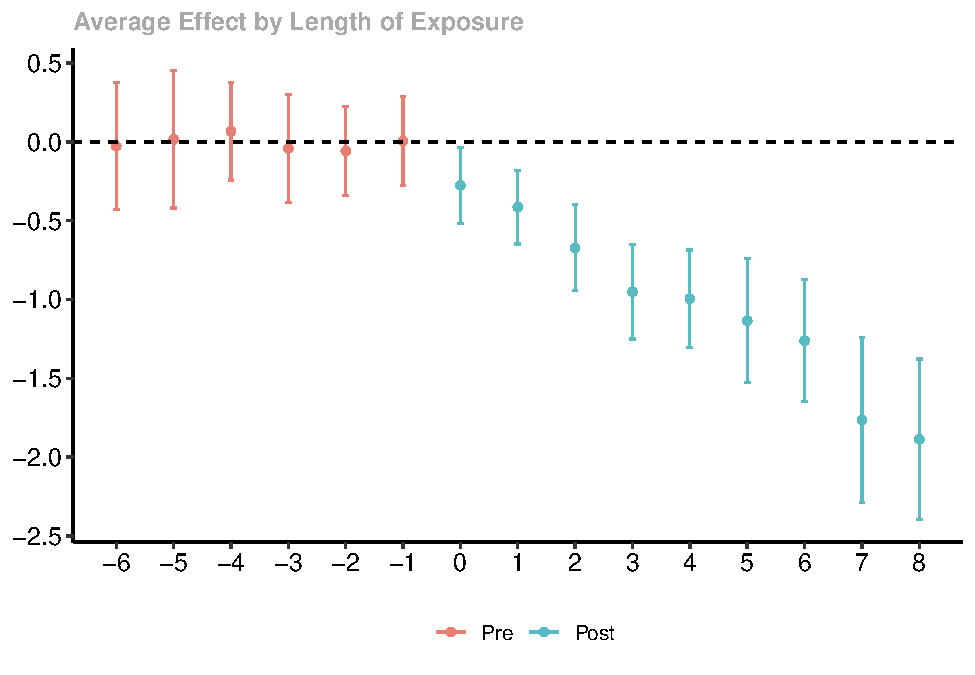
\includegraphics[width=0.85\textwidth]{Figuras/Callaway_dynamic.pdf}
\end{center}

\end{box_code}

\section{Conclusão}

O presente manual técnico sobre diferenças-em-diferenças escalonado apresenta uma análise abrangente dos principais conceitos teóricos e práticos discutidos na literatura. Ao longo deste guia, destacamos as nuances do DID escalonado, desde sua formulação básica até as contribuições mais recentes, a saber: \cite{sun2021estimating}, \cite{callaway2021difference}, \cite{de2020two} e \cite{borusyak2024revisiting}. Oferecemos, assim, orientações claras sobre quando e como aplicar cada metodologia, destacando suas diferenças e limitações.

Revisitamos a evolução do DID, comparando suas versões tradicionais com os modelos mais avançados que lidam com múltiplos períodos e tratamentos escalonados. Inicialmente, revisamos o DID padrão com dois períodos e dois grupos — um de tratamento e outro de controle. Em seguida, comparamos esse modelo com abordagens que incorporam múltiplos períodos de pré-tratamento e pós-tratamento, ainda considerando dois grupos: tratado e controle. 

Posteriormente, introduzimos o conceito de tratamento escalonado, destacando os desafios metodológicos ao se analisar esse tipo de tratamento com o modelo tradicional de DID. Em resposta, discutimos as principais soluções apresentadas na literatura recente, explorando três pilares fundamentais: o entendimento do modelo proposto, as hipóteses necessárias para garantir uma análise causal confiável e, por fim, um exemplo prático implementado em R. Além disso, na Seção \ref{sec:dif_estimadores}, detalhamos as diferenças entre os quatro principais trabalhos da literatura.

Outro ponto crucial abordado é a escolha dos pesos para agregar os efeitos do tratamento de diferentes grupos e períodos. Essa escolha deve ser guiada pela pergunta de pesquisa e realizada de forma criteriosa, evitando uma ``procura por resultados'' que comprometa a validade das conclusões. Na seção \ref{sec:definindoPesos}, detalhamos o processo de escolha dos pesos. 

Embora as metodologias apresentadas sejam robustas, é fundamental destacar que sua aplicação exige atenção especial às suposições subjacentes. Cada estudo possui características específicas que podem demandar adaptações metodológicas ou a inclusão de hipóteses adicionais.

Outro aspecto importante a ser considerado é que os exemplos fornecidos em R são simplificados e utilizam dados já tratados. Em muitas aplicações práticas, será necessário realizar o pré-tratamento de dados brutos, uma etapa essencial que não foi abordada neste manual.

Além disso, a literatura sobre diferenças-em-diferenças escalonado está em constante evolução, tornando essencial manter-se atento às novas metodologias que possam surgir. Vale destacar que há pesquisas em andamento, e até mesmo concluídas, que abordam outras estruturas de tratamento em dados em painel, não contempladas pela literatura discutida neste manual. Exemplos incluem diferenças-em-diferenças escalonado com tratamento contínuo e o controle sintético. Essas metodologias podem ser úteis, dependendo da estrutura do problema analisado, e, em alguns casos, até mesmo mais adequadas.

Esperamos que este manual sirva como um guia prático e confiável para economistas e cientistas de dados interessados em compreender e aplicar o DID escalonado. Mais do que uma simples revisão da literatura, nosso objetivo foi construir uma ponte entre a teoria e a prática, capacitando os leitores a realizar análises causais sólidas para a avaliação de políticas públicas baseadas em evidências.

    
\newpage
%\bibliographystyle{apalike}
\bibliography{Bib}

\end{document}
